\section{Problem statement and modeling rationale}\label{problem-statement-and-modeling-rationale}

\subsection{Decisions, costs, and required outputs}\label{decisions-costs-and-required-outputs}

The grid-connected microgrid meets residential demand using photovoltaic (PV) generation, purchases from the external grid, and battery storage. The battery can absorb PV surplus or low-price purchases for later use. Its losses and power limits make minimum purchased energy and minimum expenditure different objectives. Uncertain load and PV output can leave a deficit after the normal commitment has been fixed, requiring emergency purchases at five times the current tariff. The four questions in the competition statement {[}1{]} vary the information and contractual flexibility available to this system.

The supplied battery has a rated capacity of 12,000 kWh, maximum charging/discharging power of 5,000 kW, an operating energy range of 1,200-10,800 kWh, and a stated charging/discharging efficiency of 90\%. Its stored energy at 00:00 on 1 January 2025 is 6,000 kWh. Load and PV observations are in kW, prices are in CNY/kWh, and the requested purchase and battery-flow outputs are in kWh. Section 2 distinguishes these given conditions from the measurement and efficiency interpretations needed for calculation.

Figure 1 illustrates the microgrid components and energy flows shared by the four tasks. The emergency-purchase branch applies to Q2-Q4.

\begin{figure}[!htbp]
\centering
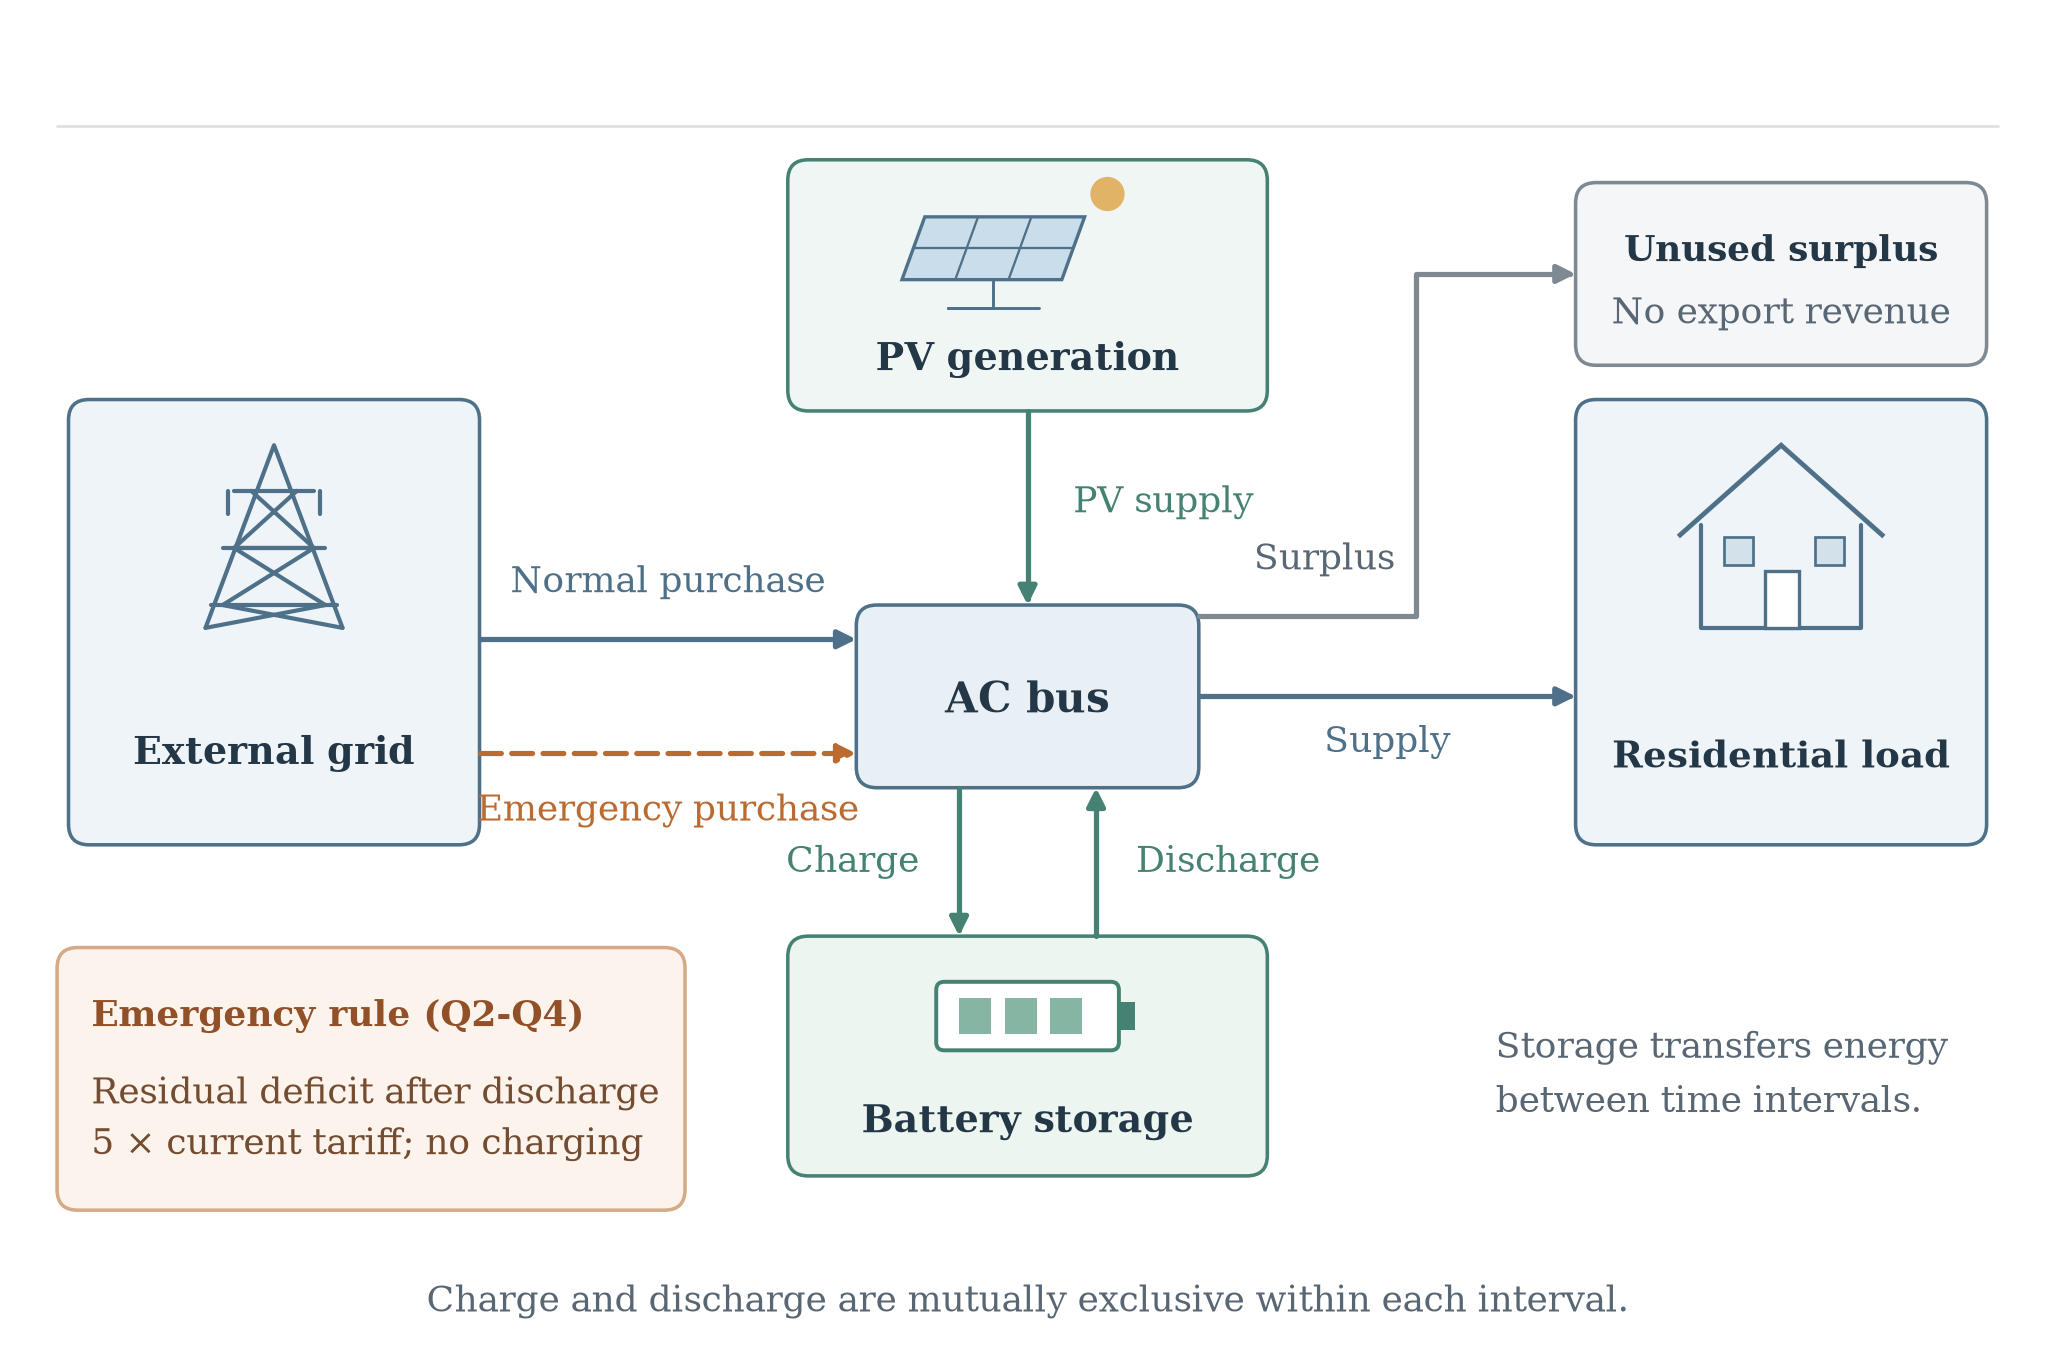
\includegraphics[width=\linewidth,height=150mm,keepaspectratio]{build/figure-01.png}
\caption{Microgrid configuration and energy flows. In Q2-Q4, emergency purchases cover demand left after discharge under the preissued storage reserve rule; they cannot charge storage. Unused surplus earns no export revenue. Arrows represent modeled energy flows, not detailed electrical wiring.}
\label{fig:1}
\end{figure}

\textbf{Q1: deterministic daily scheduling.} Attachment 1 supplies a daily load, tariff, and PV forecast profile. A purchase plan is made at midnight with equal beginning and ending stored energy. The task requires the specified interval purchases, daily purchase amount and fee, four-hour charging/discharging totals, and boundary energy in \nolinkurl{result1.xlsx}.

\textbf{Q2: a fixed commitment under uncertain load and PV.} With the repeated Attachment 1 tariff and Attachment 2 observations, the entire normal-purchase vector is fixed at midnight. During actual operation, emergency purchases cover any remaining supply deficit at five times the trading-time tariff; the normal commitment remains payable. The annual plan and realized storage and emergency-purchase records form \nolinkurl{result2.xlsx}.

\textbf{Q3: paid revision using released PV forecasts.} Attachment 3 adds 24-hour hourly PV forecasts released at 00:00, 06:00, 12:00, and 18:00. Future purchases may be revised using later releases. The statement assigns a 50\%-of-tariff breach charge to reductions and a 1.5-times-tariff price to added quantities. The model must account for these charges and emergency purchases, produce \nolinkurl{result3.xlsx}, and assess whether later forecasts justify revising the commitment.

\textbf{Q4: variable-price settlement.} Attachment 4 replaces the repeated tariff with time-varying actual prices. The Q2 and Q3 tasks are repeated as \nolinkurl{result4-2.xlsx} and \nolinkurl{result4-3.xlsx}. We interpret this extension as preserving each branch\textquotesingle s PV access and revision permissions. Planning-price alternatives are compared under the same actual-price settlement within each branch.

The five workbooks contain complete schedules. Q1 covers one supplied day; the annual branches cover 1 February-31 December 2025, or 334 days and 48,096 ten-minute intervals each. Appendix D gives every required result for 20 March, 21 June, 23 September, and 21 December, including all emergency episodes. Its captions identify the original statement requirements; paper table numbers are editorial.

\subsection{Why these model components belong together}\label{why-these-model-components-belong-together}

Battery operation couples successive intervals: charging now changes the energy available to meet a later deficit. In Q1, the supplied profiles permit a deterministic mixed-integer linear program (MILP), with linear energy accounting and binary operating modes that exclude simultaneous charging and discharging. Related battery energy-management applications use this formulation {[}2{]}.

For Q2-Q4, normal purchases and the timing of battery discharge must be assessed together. Fixing purchases does not make immediate maximum discharge economical: using storage for a low-price deficit can leave a later high-price deficit uncovered. We therefore choose a purchase vector and a time-varying reserve threshold, then evaluate the same pair on complete historical daily net-load errors. The threshold limits discharge using current energy; it does not give a scenario advance knowledge of its future. Stochastic receding-horizon microgrid control provides a precedent for combining uncertainty with updated information {[}3{]}, but does not specify this problem\textquotesingle s revision bill. An explicit final-contract cost extends the paired decision to permitted update times. Each update starts from actual stored energy, freezes executed purchases and thresholds, and can retain the complete current pair.

Table 1 links each model component to the limitation it addresses and the evidence used to assess it. We evaluate forecast changes by their effect on operating cost, using the same physical and settlement rules for each comparison.

% TABLE-BEGIN 1
\Needspace{201.8pt}
\begingroup
\fontsize{9.0}{10.8}\selectfont
\setlength{\tabcolsep}{3.2pt}
\renewcommand{\arraystretch}{1.12}
\setlength{\LTleft}{0pt plus 1fill}\setlength{\LTright}{0pt plus 1fill}
\setlength{\LTcapwidth}{\linewidth}

\begin{longtable}[]{@{}
  >{\raggedright\arraybackslash}p{(\linewidth - 6\tabcolsep) * \real{0.2495}}
  >{\raggedright\arraybackslash}p{(\linewidth - 6\tabcolsep) * \real{0.2526}}
  >{\raggedright\arraybackslash}p{(\linewidth - 6\tabcolsep) * \real{0.2526}}
  >{\raggedright\arraybackslash}p{(\linewidth - 6\tabcolsep) * \real{0.2453}}@{}}
\caption{Task structure, model choice, and planned verification.}\tabularnewline
\toprule\noalign{}
\begin{minipage}[b]{\linewidth}\raggedright
\textbf{Task structure}
\end{minipage} & \begin{minipage}[b]{\linewidth}\raggedright
\textbf{Limitation requiring attention}
\end{minipage} & \begin{minipage}[b]{\linewidth}\raggedright
\textbf{Component and purpose}
\end{minipage} & \begin{minipage}[b]{\linewidth}\raggedright
\textbf{Evidence in this paper}
\end{minipage} \\
\midrule\noalign{}
\endfirsthead
\caption[]{Task structure, model choice, and planned verification. (continued)}\tabularnewline
\toprule\noalign{}
\begin{minipage}[b]{\linewidth}\raggedright
\textbf{Task structure}
\end{minipage} & \begin{minipage}[b]{\linewidth}\raggedright
\textbf{Limitation requiring attention}
\end{minipage} & \begin{minipage}[b]{\linewidth}\raggedright
\textbf{Component and purpose}
\end{minipage} & \begin{minipage}[b]{\linewidth}\raggedright
\textbf{Evidence in this paper}
\end{minipage} \\
\midrule\noalign{}
\endhead
\bottomrule\noalign{}
\endfoot
\bottomrule\noalign{}
\endlastfoot
Battery energy couples successive intervals; charge and discharge cannot coincide & Purchasing each interval\textquotesingle s net deficit ignores storage transfer & Linear balance and energy recursion with binary operating modes & Q1 bounds, no-storage comparison, efficiency and power-side cases \\*
Purchases are frozen before uncertain supply and demand arrive & A zero predicted deficit does not imply a low realized bill; immediate discharge may consume energy valuable later & Shared purchases and reserve thresholds evaluated on complete historical daily errors & Q2 baselines and matched greedy/reserve comparisons; physical and cost checks \\*
Forecasts arrive in stages and changing a commitment costs money & New information matters only through an allowed action; free procurement revision omits fees & Remaining-day purchase and reserve updates from actual energy with final-contract settlement & Q3 no-update, energy-feedback, and new-PV comparisons within each controller \\
Actual prices fluctuate and need not be known in advance & A more elaborate price input need not improve the resulting decision & Fixed versus causal price inputs under identical actual-price settlement & Separate Q4-2 and Q4-3 price comparisons \\*
\end{longtable}

\endgroup
% TABLE-END 1

Figure 2 maps the information, decisions, and verification interfaces. Q1 solves its own deterministic MILP. Its physical constraints provide a common foundation, while its optimized battery trajectory is specific to the supplied day. Q2-Q4 share the historical-scenario objective and causal reserve execution, with the previously selected Q2 history window and cost weights inherited by the rolling and variable-price branches. A nominal MILP supplies starting values, not a trajectory that later policies must reproduce. Each annual policy propagates its own actual battery state from the common initialization.

\begin{figure}[!htbp]
\centering
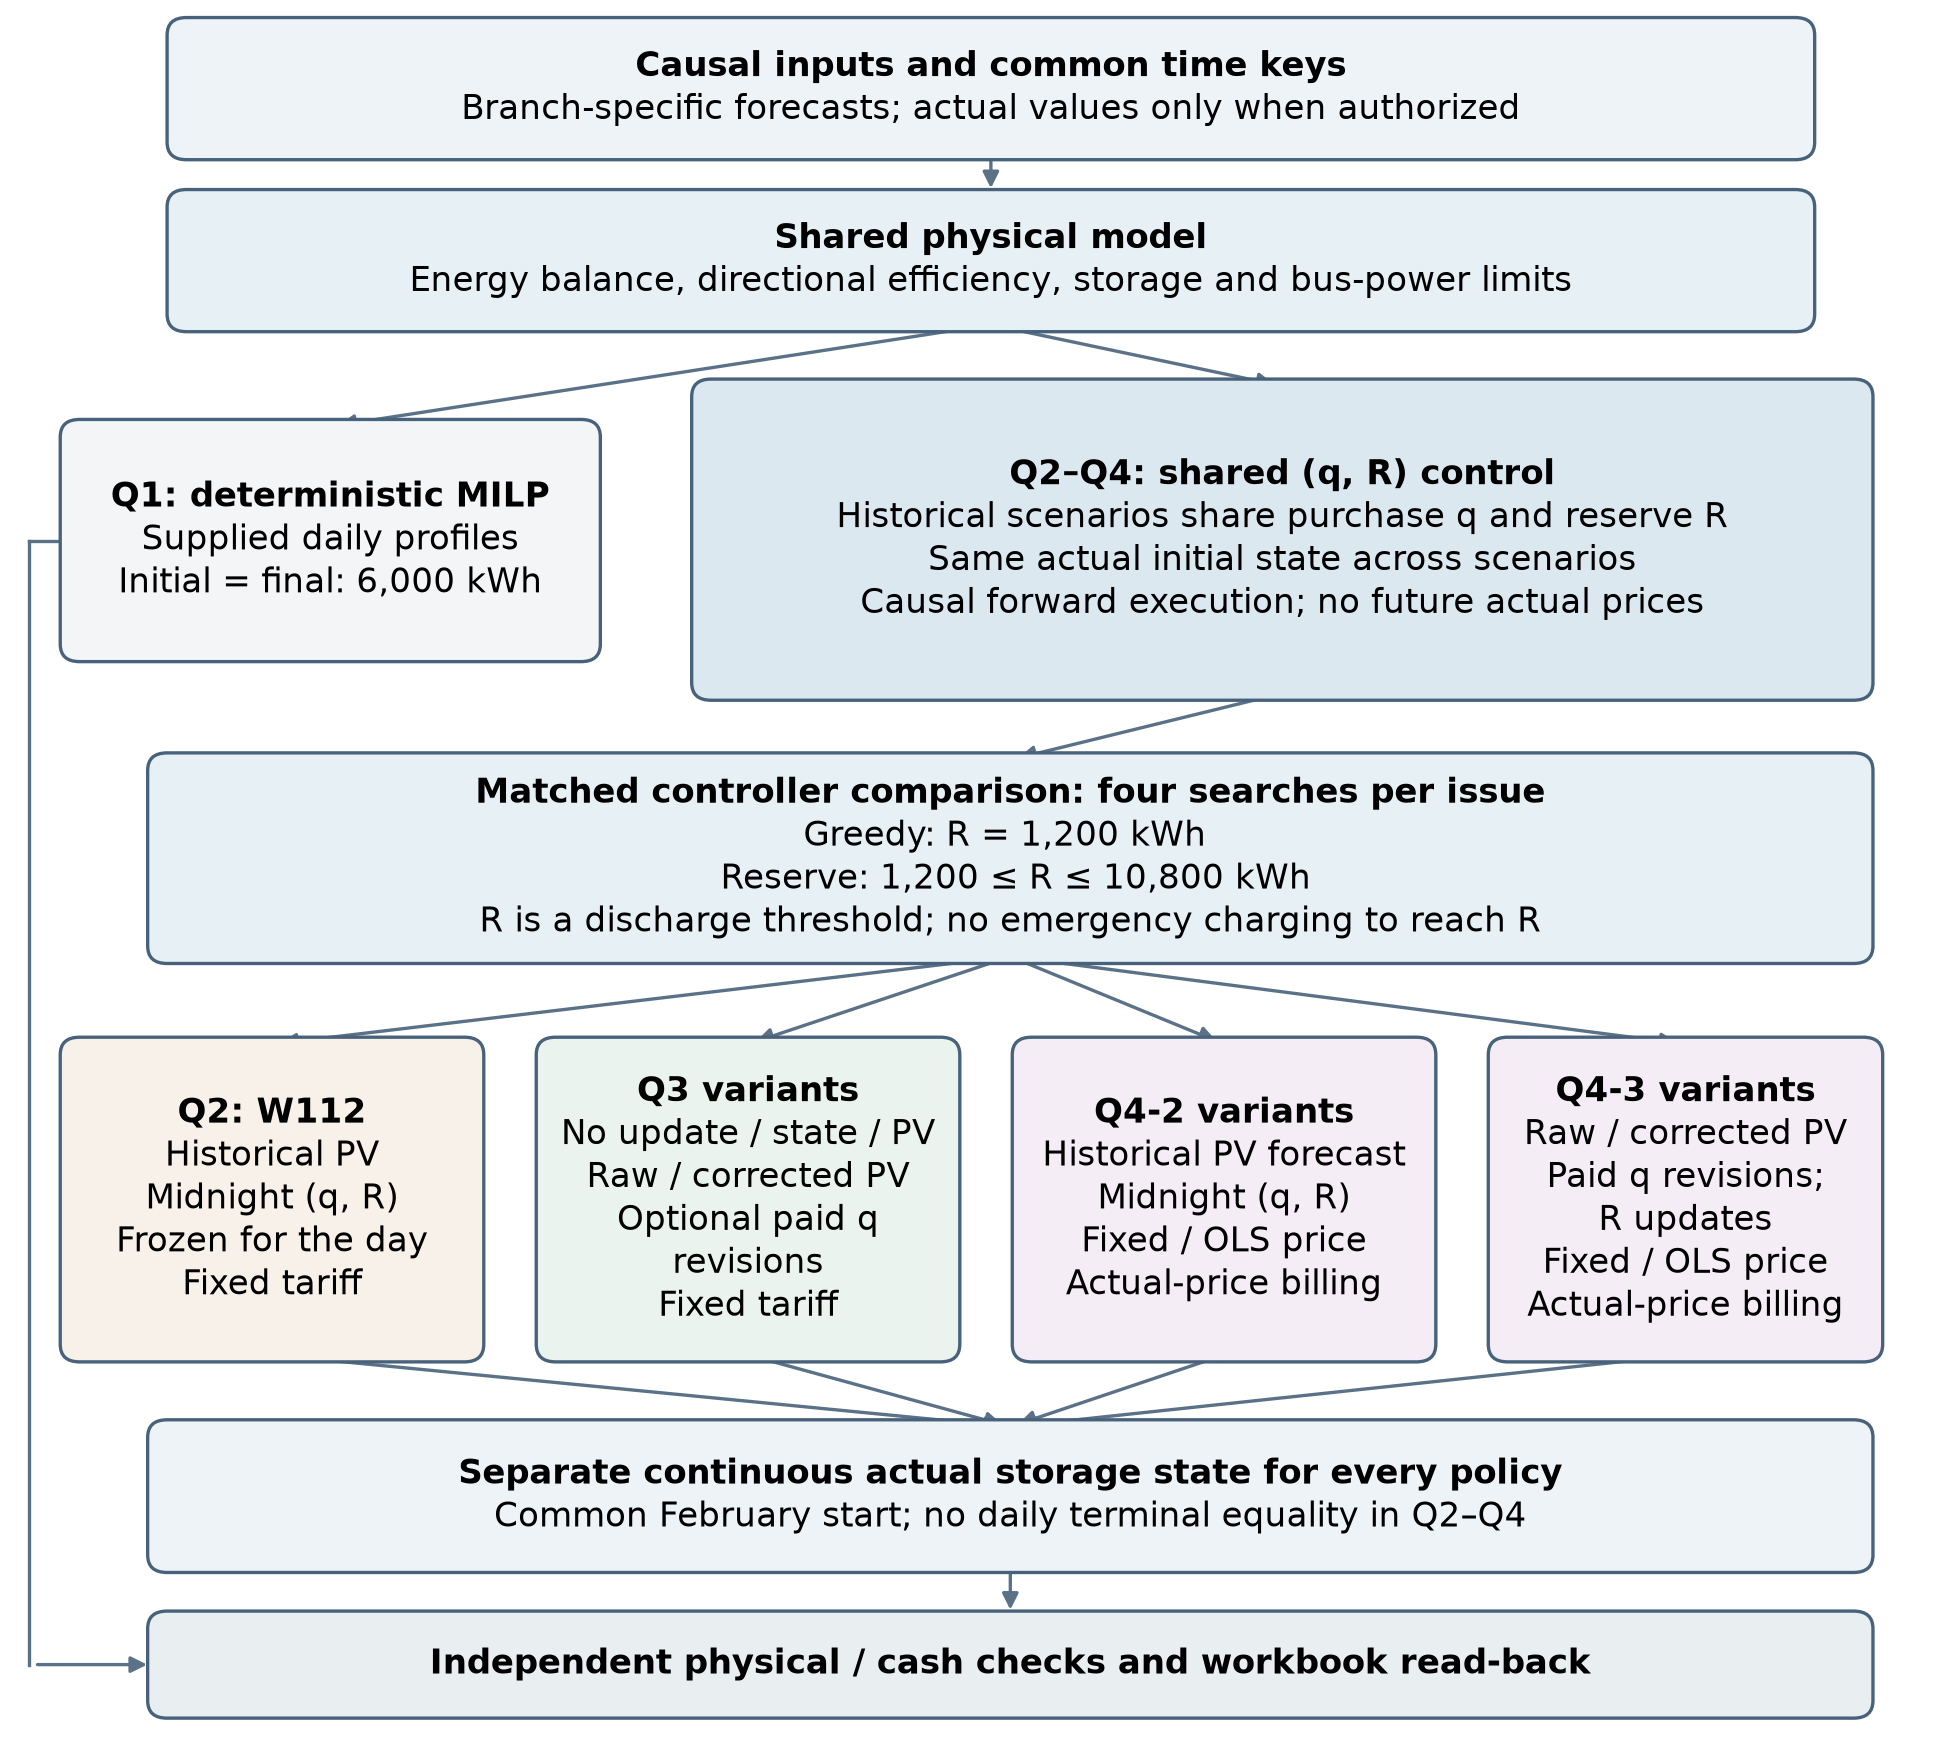
\includegraphics[width=\linewidth,height=150mm,keepaspectratio]{build/figure-02.png}
\caption{Common data and physical constraints feed an independent Q1 MILP and a shared historical-scenario purchase/reserve model for Q2-Q4. Historical-PV midnight policies and released-PV rolling policies have different information permissions. Q1 starts and ends at 6,000 kWh; annual policies carry their own actual state continuously without a daily terminal equality. Planning prices and billed prices remain distinct.}
\label{fig:2}
\end{figure}

PV bias correction is an additional candidate, retained only by historical cash ranking within the selected controller family. It does not change the common physical rules or the task-specific information permissions.

\section{Data, working interpretations, and notation}\label{data-working-interpretations-and-notation}

\subsection{Data interfaces and information cutoffs}\label{data-interfaces-and-information-cutoffs}

Attachment 1 contains 144 observations for the supplied Q1 day and the repeated reference tariff. Attachments 2 and 4 each contain 365 daily ten-minute profiles, giving 52,560 aligned actual intervals. Attachment 3 contains four releases per day with 24 hourly forecast targets per release: 1,460 releases and 35,040 release-target records. Attachment 5 supplies the workbook structures. Source workbooks remain unchanged. Derived tables retain source rows, dates, interval boundaries, and forecast issue times. We join records by explicit date-time keys and keep issue time separate from target time, so each scheduling input can be traced to its source and its availability at the decision.

Power observations in kW are multiplied by \(\Delta t=1/6\) h to obtain kWh. Tariffs already have units CNY/kWh and are not multiplied by the interval length. The retained data audit found no missing, non-numeric, or non-finite numerical entries and no negative load, PV, or price values in the input regions. All 23,540 valid zero observations in actual PV remain present. Large adjacent changes are retained and traced to source cells for review; a jump alone is insufficient evidence of a recording error. No observations are smoothed, shifted, or re-estimated for this paper.

Attachment 3 contains 1,095 blank date labels on repeated within-day forecast-release rows. These are structural labels, not missing PV forecasts. Their earlier forward filling follows the original row order and retains a transformation record without changing forecast-power values. Under the interpolation convention in Section 2.2, the first release at 00:00 on 1 January lacks an available left endpoint for its first hour. Its six ten-minute derived intervals are left unavailable. The remaining 1,459 releases each provide 144 derived intervals, giving 210,234 converted records in total. This first-release gap does not enter the required February-December output horizon. Original ten-minute labels are interpreted as interval ends and readings as interval-average power. Hourly forecast point values are interpolated linearly; the first forecast hour uses an earlier issued value at its left endpoint. These measurement conventions define the conversions, rather than being corrections to forecast values.

Figure 3 summarizes the supplied year before discussing the decision models. Daily demand and PV energy integrate all 144 ten-minute intervals, including zero-generation observations; the daily mean actual tariff is an unweighted arithmetic mean of those same intervals, not a procurement-weighted price. Calendar-month groups distinguish seasonal position from within-month daily variation. These are retrospective descriptions of all 365 supplied days, including January, rather than the 334-day policy-evaluation sample or information supplied to a midnight decision. Density estimates summarize distributions without replacing or smoothing any observed time trajectory.

\begin{figure}[!htbp]
\centering
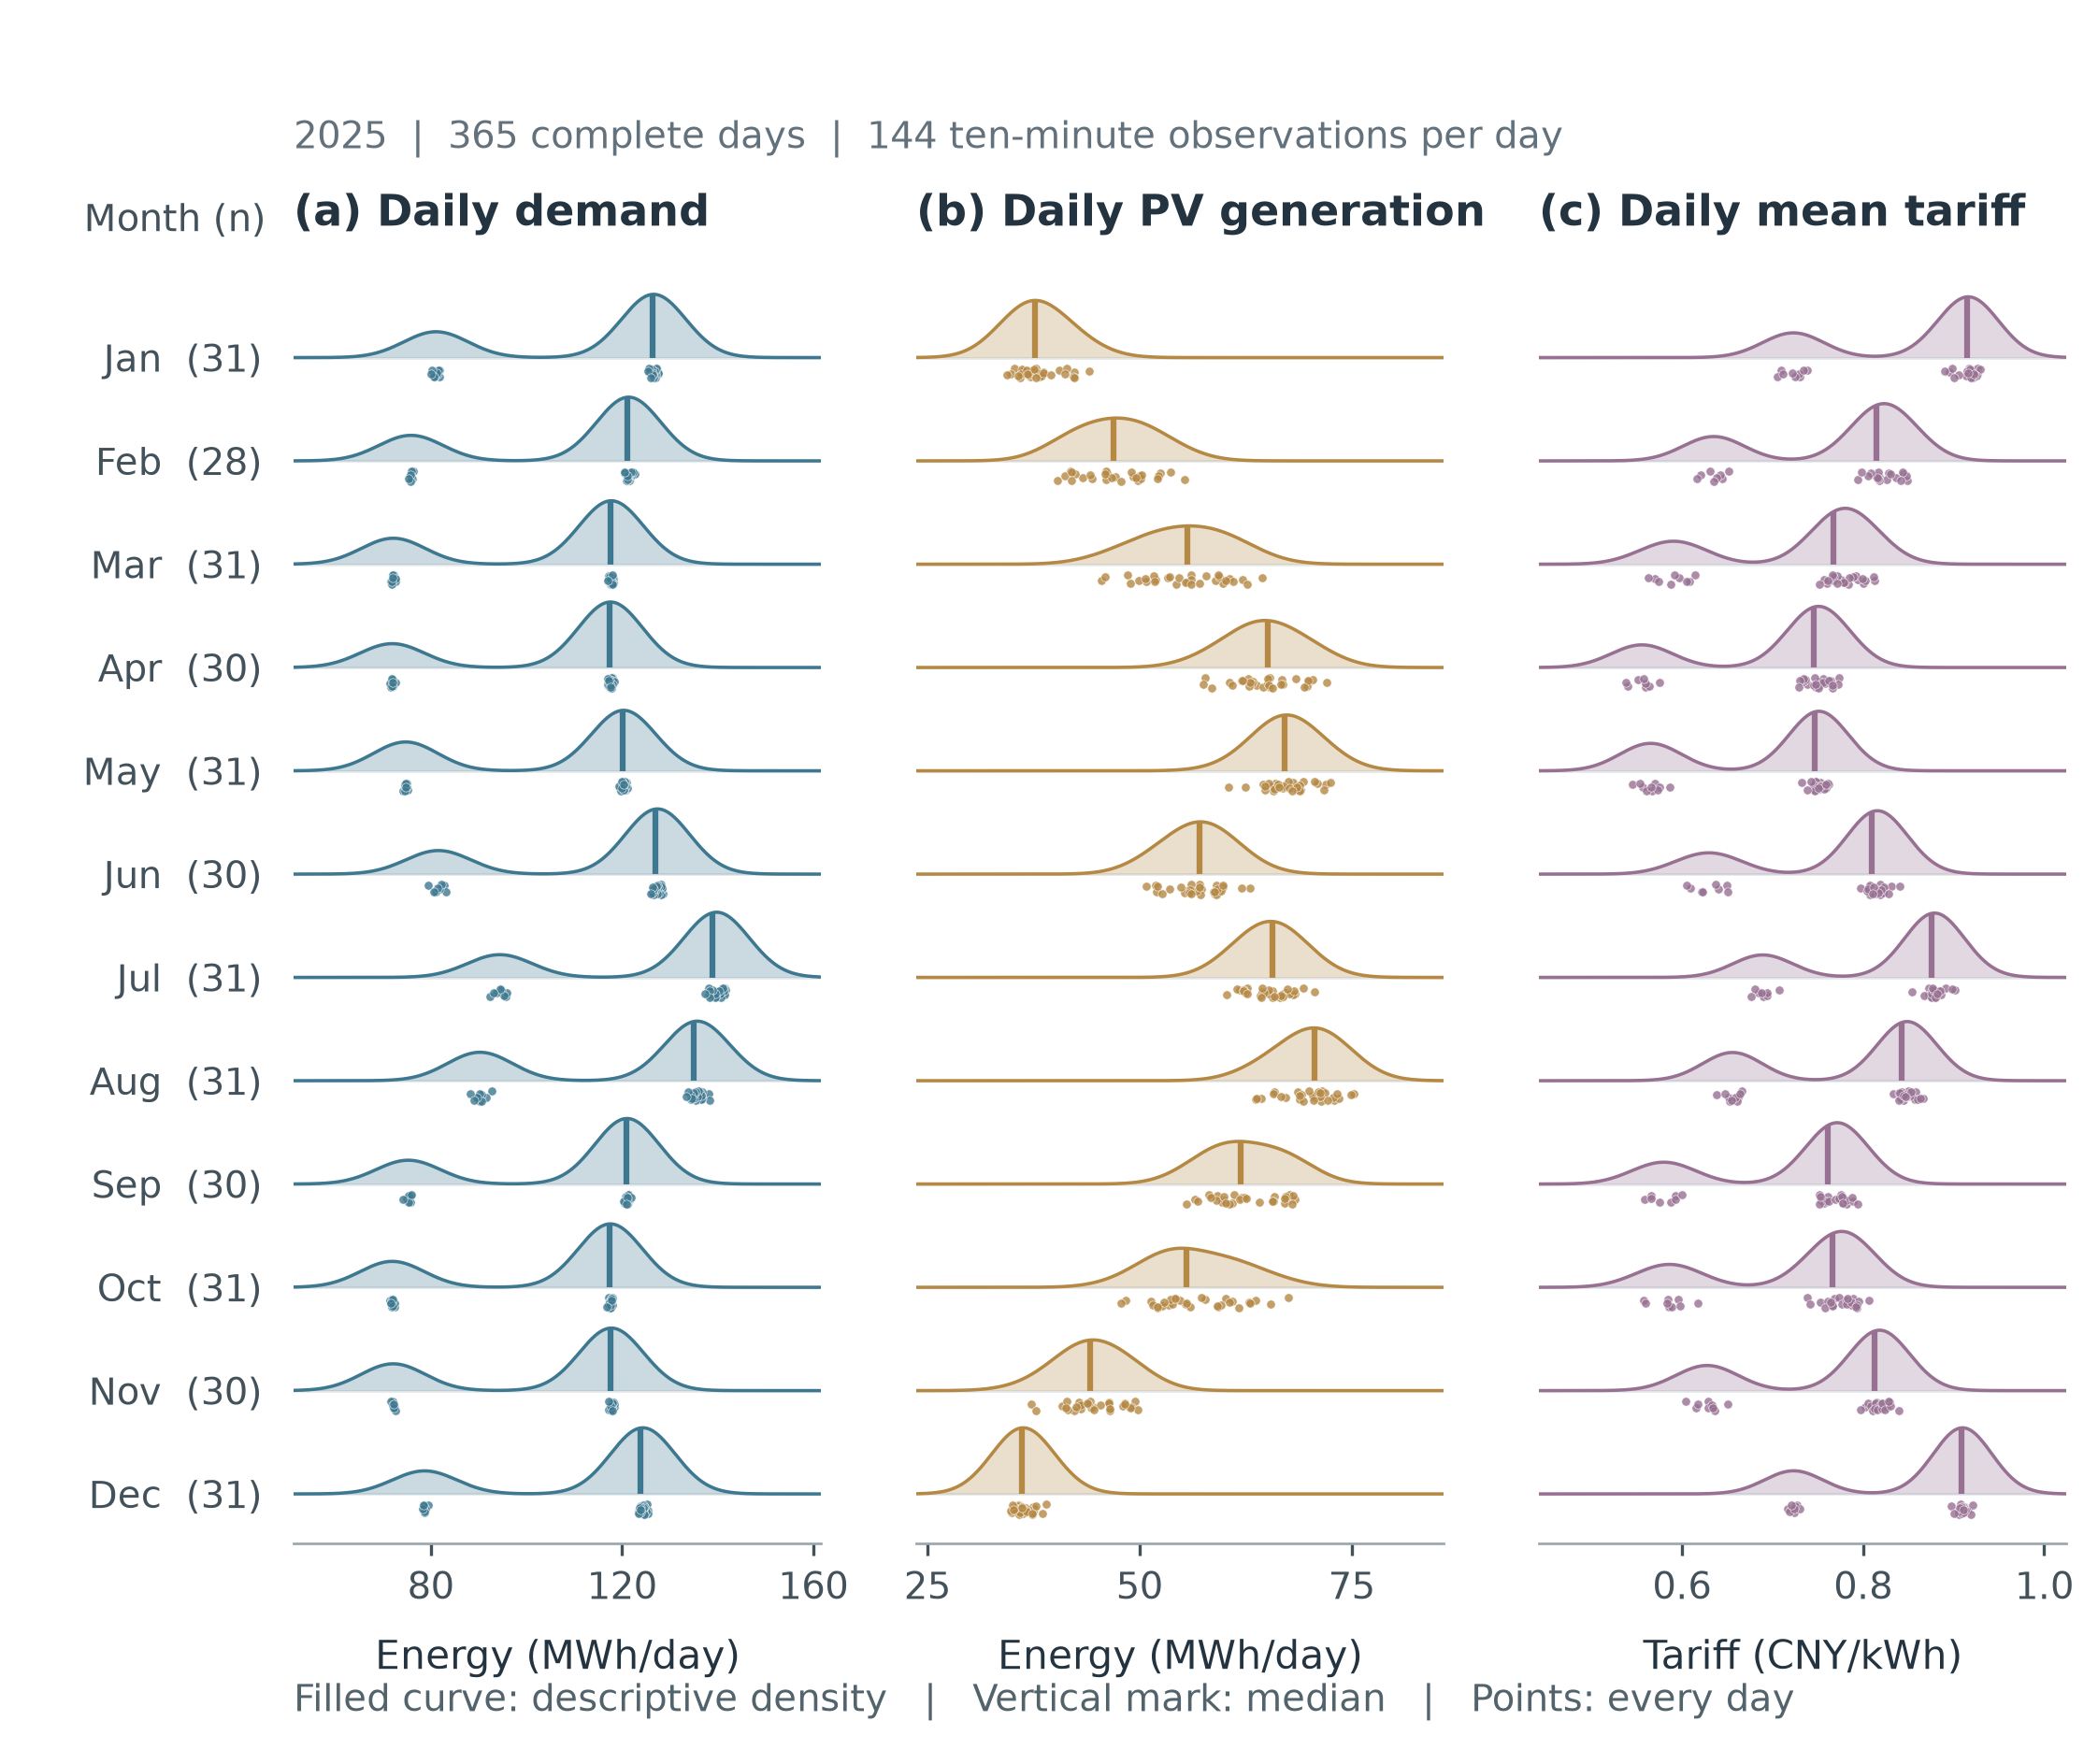
\includegraphics[width=\linewidth,height=150mm,keepaspectratio]{build/figure-03.png}
\caption{Monthly distributions across all 365 supplied days of 2025. Daily demand and PV energy use all ten-minute observations (MWh/day); mean actual tariff is the daily arithmetic mean (CNY/kWh). Original daily observations and sample counts accompany each density curve; vertical marks are monthly medians. A Scott bandwidth computed from all 365 daily values is held fixed across months within each column, with a shared density-height scale. Months stay in calendar order, and zero-PV intervals remain in daily totals. Panel scales differ by physical quantity.}
\label{fig:3}
\end{figure}

Table 2 distinguishes admissible planning inputs from subsequent actual execution data. In the annual tasks, load forecasts are fixed at midnight. A forecast for a historical date is reconstructed with that date\textquotesingle s own information cutoff, rather than with coefficients fitted later {[}4{]}.

% TABLE-BEGIN 2
\Needspace{121.8pt}
\begingroup
\fontsize{8.6}{10.32}\selectfont
\setlength{\tabcolsep}{3.2pt}
\renewcommand{\arraystretch}{1.12}
\setlength{\LTleft}{0pt plus 1fill}\setlength{\LTright}{0pt plus 1fill}
\setlength{\LTcapwidth}{\linewidth}

\begin{longtable}[]{@{}
  >{\raggedright\arraybackslash}p{(\linewidth - 8\tabcolsep) * \real{0.0800}}
  >{\raggedright\arraybackslash}p{(\linewidth - 8\tabcolsep) * \real{0.2850}}
  >{\raggedright\arraybackslash}p{(\linewidth - 8\tabcolsep) * \real{0.2650}}
  >{\raggedright\arraybackslash}p{(\linewidth - 8\tabcolsep) * \real{0.1750}}
  >{\raggedright\arraybackslash}p{(\linewidth - 8\tabcolsep) * \real{0.1950}}@{}}
\caption{Available information and adopted purchase/reserve update schedule.}\tabularnewline
\toprule\noalign{}
\begin{minipage}[b]{\linewidth}\raggedright
\textbf{Branch}
\end{minipage} & \begin{minipage}[b]{\linewidth}\raggedright
\textbf{Midnight load/PV input}
\end{minipage} & \begin{minipage}[b]{\linewidth}\raggedright
\textbf{06:00, 12:00, 18:00}
\end{minipage} & \begin{minipage}[b]{\linewidth}\raggedright
\textbf{Planning price}
\end{minipage} & \begin{minipage}[b]{\linewidth}\raggedright
\textbf{Actual settlement}
\end{minipage} \\
\midrule\noalign{}
\endfirsthead
\caption[]{Available information and adopted purchase/reserve update schedule. (continued)}\tabularnewline
\toprule\noalign{}
\begin{minipage}[b]{\linewidth}\raggedright
\textbf{Branch}
\end{minipage} & \begin{minipage}[b]{\linewidth}\raggedright
\textbf{Midnight load/PV input}
\end{minipage} & \begin{minipage}[b]{\linewidth}\raggedright
\textbf{06:00, 12:00, 18:00}
\end{minipage} & \begin{minipage}[b]{\linewidth}\raggedright
\textbf{Planning price}
\end{minipage} & \begin{minipage}[b]{\linewidth}\raggedright
\textbf{Actual settlement}
\end{minipage} \\
\midrule\noalign{}
\endhead
\bottomrule\noalign{}
\endfoot
\bottomrule\noalign{}
\endlastfoot
Q1 & Supplied deterministic daily profiles & No plan revision & Attachment 1 & Attachment 1 \\*
Q2 & Historical-data load and PV forecasts & Midnight purchases and reserve thresholds remain fixed & Attachment 1 & Attachment 1 \\*
Q3 & Midnight load forecast; current Attachment 3 PV release & Actual energy and permitted PV release; future purchases and thresholds only & Attachment 1 & Attachment 1 plus paid procurement revisions \\
Q4-2 & Q2 historical load/PV information; Attachment 3 excluded under the working interpretation in Table 3 & Midnight purchases and reserve thresholds remain fixed & Fixed reference or causal price forecast & Actual Attachment 4 prices \\
Q4-3 & Same release permissions as Q3 & Actual energy, permitted PV release, and completed price history; future purchases and thresholds only & Fixed reference or causal price forecast & Actual Attachment 4 prices plus paid procurement revisions \\*
\end{longtable}

\endgroup
% TABLE-END 2

\subsection{Working interpretations and their consequences}\label{working-interpretations-and-their-consequences}

The problem specifies energy bounds, rated power, and a 90\% efficiency, while leaving some measurement and settlement details open. Table 3 separates the supplied requirements from the working interpretations adopted in our calculations. Interval observations follow the alignment and data-quality procedures in Section 2.1.

% TABLE-BEGIN 3
\Needspace{127.4pt}
\begingroup
\fontsize{9.0}{10.8}\selectfont
\setlength{\tabcolsep}{3.2pt}
\renewcommand{\arraystretch}{1.12}
\setlength{\LTleft}{0pt plus 1fill}\setlength{\LTright}{0pt plus 1fill}
\setlength{\LTcapwidth}{\linewidth}

\begin{longtable}[]{@{}
  >{\raggedright\arraybackslash}p{(\linewidth - 4\tabcolsep) * \real{0.1838}}
  >{\raggedright\arraybackslash}p{(\linewidth - 4\tabcolsep) * \real{0.4482}}
  >{\raggedright\arraybackslash}p{(\linewidth - 4\tabcolsep) * \real{0.3680}}@{}}
\caption{Physical and accounting conventions used in the calculations.}\tabularnewline
\toprule\noalign{}
\begin{minipage}[b]{\linewidth}\raggedright
\textbf{Item}
\end{minipage} & \begin{minipage}[b]{\linewidth}\raggedright
\textbf{Adopted convention and source}
\end{minipage} & \begin{minipage}[b]{\linewidth}\raggedright
\textbf{Where it matters}
\end{minipage} \\
\midrule\noalign{}
\endfirsthead
\caption[]{Physical and accounting conventions used in the calculations. (continued)}\tabularnewline
\toprule\noalign{}
\begin{minipage}[b]{\linewidth}\raggedright
\textbf{Item}
\end{minipage} & \begin{minipage}[b]{\linewidth}\raggedright
\textbf{Adopted convention and source}
\end{minipage} & \begin{minipage}[b]{\linewidth}\raggedright
\textbf{Where it matters}
\end{minipage} \\
\midrule\noalign{}
\endhead
\bottomrule\noalign{}
\endfoot
\bottomrule\noalign{}
\endlastfoot
Battery limits & Rated capacity 12,000 kWh; operating energy 1,200-10,800 kWh, given in the statement & All state constraints \\*
Efficiency and power side & Charging and discharging efficiencies each 0.9; 5,000 kW measured at the AC bus, a working interpretation & Energy recursion and power bounds; Q1 alternatives in Section 4.2 \\*
Observation and balancing & End-of-interval observations and automatic balancing within the interval are available & Realized deficit coverage at ten-minute resolution \\
Initial and terminal energy & Q1 starts and ends at 6,000 kWh; annual policies share 7,268.4231640740745 kWh after a common January seasonal-baseline warm-up & Annual paths branch on 1 February and continue without daily/monthly resets \\
Contract settlement & The final effective quantity is settled once relative to the midnight commitment under rule A & Paid revisions in Q3/Q4-3 \\
Storage execution & Author-selected surplus charging and discharge limited by a preissued reserve threshold; the 1,200 kWh threshold recovers greedy discharge & Shared scenario and actual recursion (3); threshold policy class, not unrestricted optimal control \\
Unused energy and emergencies & Unused committed purchases remain chargeable; no export revenue; emergency energy covers the residual deficit only & Actual cash bill and surplus disposal \\
Q4-2 PV information & Preserve Q2\textquotesingle s historical-PV information set when recalculating it under variable prices; an author interpretation, not an explicit branch-specific ban on Attachment 3 & Q4-2 input construction and matched planning-price comparisons \\
Variable-price information & Future realized prices are unavailable to planning unless already observed & Causal price inputs and actual-price rebilling \\*
\end{longtable}

\endgroup
% TABLE-END 3

A common seasonal-baseline warm-up runs from 1 to 31 January, starting at the statement\textquotesingle s 6,000 kWh. Its 1 January cold start uses zero normal planned purchases; subsequent January purchases follow that baseline. The retained 4,464-interval record ends at 7,268.4231640740745 kWh, which becomes the shared 1 February initial state (Appendix A). The compared annual policies branch from this state; it is not the outcome of running each final policy separately through January. Thereafter, each policy carries its own actual energy across every midnight and month boundary. Q1\textquotesingle s equality of initial and terminal energy is required by its task. In Q2-Q4, a nominal zero-deficit trajectory and terminal energy of 1,200 kWh constrain the MILP initializer only. They do not constrain the final purchase/reserve pair, and actual storage is never reset to that level.

The efficiency and power-side conventions specify where losses occur in the energy recursion. Applying 90\% in each direction gives a different usable transfer from a symmetric 90\% round-trip interpretation; locating the power limit inside the battery also changes the bus-flow bounds. Section 4.2 compares these interpretations for Q1. The no-export convention is needed because the statement gives no selling tariff. Q1 permits only PV curtailment, whereas Q2-Q4 may also dispose of unused committed purchases that remain chargeable. Emergency purchases supply only the deficit left by the adopted discharge rule and cannot charge the battery for arbitrage.

The commitment and settlement conventions connect a causal decision to its realized bill. At each decision time, the model can use completed actual observations, released forecasts, current actual stored energy, and admissible price information. The original purchase commitment stays fixed in Q2 and Q4-2; we also fix the day\textquotesingle s reserve thresholds at midnight as a controller-design choice. Q3 and Q4-3 may update future purchases and thresholds at their permitted decision times. Rule A settles each interval\textquotesingle s final effective purchase quantity once against its midnight commitment; earlier versions are not added as separate purchases. No separate reserve-change fee is introduced, because the contract charges concern grid quantities and no storage switching cost is supplied. Section 3 gives the exact refund-and-breach-charge treatment. Future actual prices are withheld from planning, while actual Attachment 4 prices determine Q4 settlement.

\Needspace{5\baselineskip}

Within a forecast hour, let \(a\) and \(b\) denote consecutive forecast target times, with power values \(\widehat P_a\) and \(\widehat P_b\). For any ten-minute interval \(I_t\) within that hour, the generation input is

\[
\widehat G_t=\int_{I_t}\left[\widehat P_a+
\frac{\tau-a}{b-a}(\widehat P_b-\widehat P_a)\right]d\tau. \tag{1}
\]

Time in (1) is measured in hours, giving kWh. Only issued values are used. A release contains 24 hours of forecasts, but the current optimization uses only intervals up to the current day\textquotesingle s 24:00. The implications of this remaining-day horizon are discussed in Section 9.

A single internal energy state represents the battery. We omit self-discharge, degradation charges, ramping limits, network constraints, communications cost, and sub-interval converter dynamics because the task supplies no parameters for them. The model retains capacity, efficiency, power limits, and energy transfer between intervals. It describes interval-level scheduling; it has not been validated as a physical controller operating on a seconds scale. Historical cost calculations require no assumption of normal, independent, or stationary errors, and the empirical scenario average does not establish those properties.

\subsection{Symbols and units}\label{symbols-and-units}

At release stage \(k\in\{0,1,2,3\}\), the clock time is \(6k\) hours and the first unexecuted ten-minute interval is \(\tau_k=36k\). Thus \(\mathcal T_k=\{\tau_k,\ldots,143\}\). Q2 and Q4-2 use only \(k=0\). A scenario at stage \(k\) starts from the actual boundary state \(E^{\mathrm{act}}_{d,\tau_k}\); \(k\) is a release index, whereas the subscript of \(E_t\) always denotes a physical interval boundary. Previously executed quantities for \(t<\tau_k\) are fixed. Suppress \(d,k\) only within one decision.

Table 4 collects quantities shared by the models. Stored energy \(E\) is measured inside the battery, whereas charging and discharging flows are measured at the bus.

% TABLE-BEGIN 4
\Needspace{116.8pt}
\begingroup
\fontsize{9.0}{10.8}\selectfont
\setlength{\tabcolsep}{3.2pt}
\renewcommand{\arraystretch}{1.12}
\setlength{\LTleft}{0pt plus 1fill}\setlength{\LTright}{0pt plus 1fill}
\setlength{\LTcapwidth}{\linewidth}

\begin{longtable}[]{@{}
  >{\raggedright\arraybackslash}p{(\linewidth - 4\tabcolsep) * \real{0.2500}}
  >{\raggedright\arraybackslash}p{(\linewidth - 4\tabcolsep) * \real{0.5900}}
  >{\raggedright\arraybackslash}p{(\linewidth - 4\tabcolsep) * \real{0.1600}}@{}}
\caption{Main notation.}\tabularnewline
\toprule\noalign{}
\begin{minipage}[b]{\linewidth}\raggedright
\textbf{Symbol}
\end{minipage} & \begin{minipage}[b]{\linewidth}\raggedright
\textbf{Meaning}
\end{minipage} & \begin{minipage}[b]{\linewidth}\raggedright
\textbf{Unit}
\end{minipage} \\
\midrule\noalign{}
\endfirsthead
\caption[]{Main notation. (continued)}\tabularnewline
\toprule\noalign{}
\begin{minipage}[b]{\linewidth}\raggedright
\textbf{Symbol}
\end{minipage} & \begin{minipage}[b]{\linewidth}\raggedright
\textbf{Meaning}
\end{minipage} & \begin{minipage}[b]{\linewidth}\raggedright
\textbf{Unit}
\end{minipage} \\
\midrule\noalign{}
\endhead
\bottomrule\noalign{}
\endfoot
\bottomrule\noalign{}
\endlastfoot
\hspace{0.5pt}\(d,t,k,s\) & Operating day; ten-minute interval \(t=0,\ldots,143\); decision stage; completed historical scenario day & Index \\*
\hspace{0.5pt}\(\tau_k,\mathcal T_k\) & First unexecuted boundary \(\tau_k=36k\); remaining intervals \(\{\tau_k,\ldots,143\}\) & Index, set \\*
\hspace{0.5pt}\(H_{d,k}\) & Eligible completed historical days within the preceding \(W\) calendar days & Set \\
\hspace{0.5pt}\(L_t,G_t\) & Community load energy and PV generation energy in interval \(t\) & kWh \\
\hspace{0.5pt}\(\widehat L_{d,t,00}\) & Load-energy forecast for day \(d\), interval \(t\), fixed at midnight & kWh \\
\hspace{0.5pt}\(\widehat G_{d,t,k}\) & PV-energy forecast for day \(d\), interval \(t\), available at stage \(k\) & kWh \\
\hspace{0.5pt}\(q_t^0\) & Original normal-purchase commitment made at midnight for interval \(t\) & kWh \\
\hspace{0.5pt}\(q_t^k\) & Normal-purchase commitment for interval \(t\) after stage \(k\) & kWh \\
\hspace{0.5pt}\(\bar q_t\) & Final effective normal-purchase commitment executed in interval \(t\) & kWh \\
\hspace{0.5pt}\(R_t^0,R_t^k,\bar R_t\) & Discharge reserve threshold issued at midnight, updated at stage \(k\), and finally applied in interval \(t\) & kWh \\
\hspace{0.5pt}\(c_t\) & Energy charged from the microgrid bus into the battery in interval \(t\) & kWh \\
\hspace{0.5pt}\(b_t\) & Energy discharged from the battery to the microgrid bus in interval \(t\) & kWh \\
\hspace{0.5pt}\(u_t\) & Emergency purchase covering the remaining supply deficit in interval \(t\) & kWh \\
\hspace{0.5pt}\(w_t\) & Unused surplus disposed of without sale revenue in interval \(t\) & kWh \\
\hspace{0.5pt}\(E_t\) & Stored energy at the beginning of interval \(t\) & kWh \\
\hspace{0.5pt}\(p^{\mathrm{plan}}_{t\mid k},p^{\mathrm{act}}_t\) & Price used for planning; price used for actual settlement & CNY/kWh \\
\hspace{0.5pt}\(P\) & Bus-side charge/discharge energy limit per ten-minute interval, \(5000/6\) & kWh \\
\hspace{0.5pt}\(\eta_c,\eta_d\) & Charging and discharging efficiencies, respectively & Dimensionless \\
\hspace{0.5pt}\(r^s_{t,k},n^s_{d,t,k}\) & Historical net forecast error; scenario net load & kWh \\
\hspace{0.5pt}\(W\) & Length of the calendar window used to select completed historical days & day \\
\hspace{0.5pt}\(\kappa\) & Emergency-cost weight in the empirical planning objective & Dimensionless \\
\hspace{0.5pt}\(\mu\) & Fixed terminal-inventory value proxy in the planning objective & CNY/kWh \\
\hspace{0.5pt}\(\nu\) & Common terminal-energy valuation used only in the historical inventory audit & CNY/kWh \\
\hspace{0.5pt}\(F_A\) & Final rule-A contract cost relative to the midnight commitment & CNY \\
\hspace{0.5pt}\(J_k\) & Remaining-horizon empirical planning objective at stage \(k\) & CNY \\*
\end{longtable}

\endgroup
% TABLE-END 4

The positive part is \((x)_+=\max(x,0)\). Day and stage subscripts are suppressed when the context fixes them. Unadorned \(q\) and \(R\) denote the candidate purchase and reserve vectors. Both are shared across scenarios; scenario-specific energy states and emergency quantities arise only by forward execution of that common policy.

\section{Common execution model and joint purchase/reserve objective}\label{common-execution-model-and-joint-purchasereserve-objective}

\subsection{Physical execution and historical scenarios}\label{physical-execution-and-historical-scenarios}

\Needspace{5\baselineskip}

Let \(q_t\) be the effective normal purchase in interval \(t\). At the AC bus, normal purchases, PV, discharge \(b_t\), and emergency purchases \(u_t\) meet load and charging \(c_t\); residual surplus \(w_t\) is disposed of without revenue. The common balance and battery recursion are

\[
q_t+G_t+b_t+u_t=L_t+c_t+w_t,\qquad
E_{t+1}=E_t+\eta_c c_t-b_t/\eta_d. \tag{2}
\]

Stored energy remains in \([1200,10800]\) kWh, and \(0\le c_t,b_t\le P=5000/6\) kWh. Q1 jointly optimizes purchases and battery actions and sets \(u_t=0\) and \(0\le w_t\le G_t\). Its particular optimizer output must not be confused with the following rule for uncertain realized operation.

\Needspace{5\baselineskip}

For Q2-Q4, let \(v_t=q_t+G_t-L_t\) be the realized pre-storage surplus. Along with purchases, choose a discharge reserve threshold \(R_t\in[1200,10800]\) kWh before executing the interval. Surplus charging remains limited by current surplus, power, and capacity. During a deficit, only energy above the threshold may be discharged:

\[
\begin{aligned}
c_t&=\min\{(v_t)_+,P,(10800-E_t)/\eta_c\},\\
b_t&=\min\{(-v_t)_+,P,\eta_d(E_t-R_t)_+\},\\
u_t&=((-v_t)_+-b_t)_+,\qquad w_t=(v_t-c_t)_+.
\end{aligned} \tag{3}
\]

The threshold is a discharge rule, not a new state constraint \(E_t\ge R_t\). If current energy is below it, discharge is zero; emergency purchases do not refill the battery to the threshold. Setting every \(R_t=1200\) recovers the previous greedy executor. A larger threshold can preserve energy for later deficits while increasing the current emergency purchase, so its economic value must be measured over the full path. The sign of \(v_t\) prevents simultaneous charging and discharging. Surplus may include unused paid purchases as well as PV, with no sale credit. Equations (2)-(3) enforce the physical energy and power limits for any finite \(q\ge0\) and \(1200\le R\le10800\), starting from a physically admissible state.

\Needspace{5\baselineskip}

The joint objective must anticipate how errors deplete or refill storage over successive intervals. Let \(H_{d,k}\) contain eligible completed days in the preceding \(W\) calendar days with their contemporaneous forecast records. For historical day \(s\), define

\[
r^s_{t,k}=(L_t^s-G_t^s)
 -(\widehat L_{s,t,00}-\widehat G_{s,t,k}),\qquad
n^s_{d,t,k}=\widehat L_{d,t,00}-\widehat G_{d,t,k}+r^s_{t,k}. \tag{4}
\]

Q2 and Q4-2 use historical-data PV forecasts. Q3 and Q4-3 match the authorized PV release stage; an energy-feedback-only comparison still uses the midnight PV version. All residuals are from completed historical dates. The available pool is shorter than \(W\) near the beginning of the evaluation period; future days are never used to fill the window.

Each scenario retains its observed within-day error order. We simulate the same remaining pair \((q,R)\) against every \(n^s\) using (2)-(3), starting from the policy\textquotesingle s current actual energy. Each next state depends on that scenario\textquotesingle s current net load and preceding state. Scenarios share purchases and reserve thresholds, and execution uses no later PV release or future actual price. Allowing a separate dispatch with knowledge of each scenario\textquotesingle s future would produce an anticipatory benchmark. The empirical sample-average construction {[}5{]} lets us evaluate a time-varying threshold policy with common decisions. The windows overlap, and the search is finite and nonsmooth. Section 8 discusses the scope of the empirical comparisons, including the absence of a shuffled-scenario test.

\Needspace{100pt}

\subsection{Complete empirical program and settlement}\label{complete-empirical-program-and-settlement}

\Needspace{5\baselineskip}

For known scenario net loads from (4), the complete remaining-day program is given below. The free decisions \(q,R\) are common to all scenarios; each scenario has its own forward-recursive storage and emergency quantities. Previously executed intervals are fixed.

\[
\begin{aligned}
\min_{q,R}\quad J_k(q,R)={}
 &\sum_{t\in\mathcal T_k}C_{t,k}(q_t)
 +\frac{\kappa}{|H_{d,k}|}\sum_{s\in H_{d,k}}\sum_{t\in\mathcal T_k}p^{\mathrm{plan}}_{t\mid k}u_t^s
\\
 &-\frac{\mu}{|H_{d,k}|}\sum_{s\in H_{d,k}}(E_{144}^s-E^{\mathrm{act}}_{d,\tau_k})\\
\text{subject to}\quad
 &v_t^s=q_t-n_t^s,\quad E_{\tau_k}^s=E^{\mathrm{act}}_{d,\tau_k},\\
 &c_t^s=\min\{(v_t^s)_+,P,(10800-E_t^s)/\eta_c\},\\
 &b_t^s=\min\{(-v_t^s)_+,P,\eta_d(E_t^s-R_t)_+\},\\
 &u_t^s=((-v_t^s)_+-b_t^s)_+,\quad w_t^s=(v_t^s-c_t^s)_+,\\
 &q_t+b_t^s+u_t^s=n_t^s+c_t^s+w_t^s,\\
 &E_{t+1}^s=E_t^s+\eta_c c_t^s-b_t^s/\eta_d,\\
 &q_t\ge0,\quad1200\le R_t\le10800,\quad0\le c_t^s,b_t^s\le P,\quad u_t^s,w_t^s\ge0,\\
 &1200\le E_j^s\le10800\quad(j=\tau_k,\ldots,144),\\
 &s\in H_{d,k},\quad t\in\mathcal T_k,\quad P=5000/6,\quad\eta_c=\eta_d=0.9.
\end{aligned} \tag{5}
\]

Only \(q,R\) are free policy decisions; the displayed execution quantities are determined by recursion. There is no terminal-energy equality. Greedy controls add \(R_t=1200\); the reserve family permits the displayed interval. Algorithm 1 only approximates this nonsmooth program and does not certify its global minimum.

At midnight, \(C_{t,0}(q_t)=p^{\mathrm{plan}}_{t\mid0}q_t\). The emergency weight \(\kappa=5\) makes the middle term equal to the mean full fivefold emergency bill. Other weights are historical Q2 sensitivity candidates, not alternative settlement prices. The inherited \(\mu=0.38232\) CNY/kWh values retained energy in the planning objective; it is neither cash revenue nor an identified Bellman value function. The actual bill never subtracts this term.

\Needspace{5\baselineskip}

For an intraday revision, the normal term is the final rule-A contract cost relative to the midnight commitment:

\[
F_A(\bar q_t;q_t^0,p_t)=p_tq_t^0
 +1.5p_t(\bar q_t-q_t^0)_+
 -0.5p_t(q_t^0-\bar q_t)_+. \tag{6}
\]

Thus \(C_{t,k}(q_t)=F_A(q_t;q_t^0,p^{\mathrm{plan}}_{t\mid k})\) at a paid update. The negative term implements the adopted net reduction adjustment. Reducing a one-kWh midnight commitment to zero leaves a half-price charge; increasing it to two kWh yields \(2.5p_t\). These charges implement the working settlement interpretation in Table 3.

\Needspace{5\baselineskip}

Only the final effective quantity for each interval is billed, once. Earlier versions are not cumulatively added, and executed intervals are frozen. The realized bills are therefore

\[
\begin{aligned}
B_{\mathrm{Q2/Q42}}&=\sum_t p_t^{\mathrm{act}}(q_t^0+5u_t),\\
B_{\mathrm{Q3/Q43}}&=\sum_t\left[
F_A(\bar q_t;q_t^0,p_t^{\mathrm{act}})+5p_t^{\mathrm{act}}u_t\right].
\end{aligned} \tag{7}
\]

The emergency multiplier is the entire price \(5p\), not an extra \(5p\) on top of the normal price. Q4 uses the actual Attachment 4 price in both components of (7), regardless of the planning price in (5). For Q1-Q3 the applicable actual tariff is the repeated Attachment 1 tariff.

\subsection{Nominal initialization and candidate search}\label{nominal-initialization-and-candidate-search}

A deterministic MILP supplies a nominal starting trajectory. The minimum operators in (3), the reserve boundary, and the contract kink at \(q=q^0\) make the shared objective (5) nonsmooth. Limited-memory bound-constrained search {[}6{]} generates candidates that are explicitly retained and rescored; its stopping status is not an optimality certificate. The SciPy interface supplies the bounds and termination controls {[}7{]}. The comparison gives both the reserve and greedy controllers four searches per decision, so adding two search starts alone is not counted as evidence for improved storage control.

\Needspace{5\baselineskip}

The initializer uses a separate 28-day residual pool. For each clock hour, \(\delta_t\) is the linear-interpolated empirical quantile of all available residuals within that hour, with levels 0.85 for 09:00-11:00, 0.65 for 11:00-18:00, 0.95 for 18:00-22:00, and 0.80 otherwise. Let \(\widetilde L_t=(\widehat L_{d,t,00}+\delta_t)_+\) and \(\widetilde G_t=\widehat G_{d,t,k}+(-\widehat L_{d,t,00}-\delta_t)_+\). These preserve the risk-adjusted net load, including negative net values. With tildes denoting nominal rather than executed variables, solve

\[
\begin{aligned}
\min\quad&\sum_{t\in\mathcal T_k}\widetilde C_{t,k}(\widetilde q_t)\\
\text{subject to}\quad
 &\widetilde q_t+\widetilde G_t+\widetilde b_t=\widetilde L_t+\widetilde c_t+\widetilde w_t,\\
 &\widetilde E_{t+1}=\widetilde E_t+\eta_c\widetilde c_t-\widetilde b_t/\eta_d,\\
 &\widetilde E_{\tau_k}=E^{\mathrm{act}}_{d,\tau_k},\quad\widetilde E_{144}=1200,\\
 &1200\le\widetilde E_j\le10800\quad(j=\tau_k,\ldots,144),\\
 &0\le\widetilde c_t\le Pz_t,\quad0\le\widetilde b_t\le P(1-z_t),\quad z_t\in\{0,1\},\\
 &\widetilde q_t\ge0,\quad\widetilde w_t\ge0,\quad
 \widetilde w_t\le\widetilde G_t\ \text{if }k=0,\qquad t\in\mathcal T_k.
\end{aligned} \tag{8}
\]

At midnight, \(\widetilde C_{t,0}=p^{\mathrm{plan}}_{t\mid0}\widetilde q_t\). At a paid update, \(\widetilde C_{t,k}=F_A(\widetilde q_t;q_t^0,p^{\mathrm{plan}}_{t\mid k})\): the MILP introduces a nonnegative fee variable \(y_t\) and minimizes \(\sum_ty_t\) subject to \(y_t\ge1.5p_t\widetilde q_t-0.5p_tq_t^0\) and \(y_t\ge0.5p_t\widetilde q_t+0.5p_tq_t^0\), using planning prices here. Intraday surplus has no PV-only upper bound because the inherited remaining-horizon implementation permits disposal of paid grid energy. The initializer contains no emergency purchase. Its zero-deficit balance, binary nominal dispatch and terminal target apply only to its starting trajectory. The final empirical program does not inherit those restrictions. Algorithm 1 uses \(\widetilde q\) and, for one reserve start, clipped nominal end-of-interval energies; fallback behavior remains unchanged.

\Needspace{5\baselineskip}

\textbf{Algorithm 1. Joint purchase/reserve decision at an authorized stage.}

\begin{enumerate}
\def\labelenumi{\arabic{enumi}.}
\tightlist
\item
  Read the policy\textquotesingle s actual energy and available information. Freeze both purchases and reserve thresholds for executed intervals.
\item
  Form release-matched historical scenarios using (4). Every candidate starts from the same current actual energy.
\item
  Construct a risk-profile MILP purchase start and a positive point-net-load start. Run two purchase-only L-BFGS-B searches with \(R=1200\), retaining each start, best evaluated point, and returned point: six greedy candidates.
\item
  Start two additional searches from the risk-profile purchase vector and the best of those six purchase vectors. In the reserve arm, their reserve starts are the MILP\textquotesingle s nominal end-of-interval energies clipped to \([1200,10800]\), and the constant 1,200 vector, respectively. Use the constant vector if the initializer has no energy trajectory. In the matched greedy arm, both additional searches keep \(R=1200\).
\item
  Retain each additional start, best evaluated pair, and returned pair. Rescore all twelve candidates with (5). At an intraday update, append the complete unchanged current pair \((q,R)\) as candidate thirteen. Select the first score within \(10^{-8}\) CNY of the minimum in this fixed order.
\item
  Apply the selected future purchases and thresholds, execute (3) until the next allowed decision, and carry actual energy forward. Settle final effective purchase quantities once using (7).
\end{enumerate}

The nominal energy trajectory supplies only a starting threshold vector; final purchases, reserve thresholds, and realized day-end energy need not reproduce it.

The adopted parameters remain \(W=112\), \(\kappa=5\), and \(\mu=0.38232\), inherited from the earlier Q2 study without retuning. Every search uses \nolinkurl{maxiter=180}, \nolinkurl{maxfun=1600}, \nolinkurl{maxls=30}, \nolinkurl{maxcor=10}, \nolinkurl{ftol=1e-10}, and \nolinkurl{gtol=1e-5}. Procurement coordinates are scaled as \(q/1000\), reserve coordinates as \((R-1200)/1000\), and the objective as \(J/10000\). Joint searches use derivatives with respect to both vectors; rule A changes only the procurement part of the gradient. The compiled forward and backward recursion evaluates the same model. At nonsmooth ties it uses recorded branch derivatives, including the intermediate contract slope \(p\) at \(q=q^0\); these choices do not imply differentiability. Appendix A identifies code and configuration records.

Keeping the six original greedy candidates means the selected pair cannot have a worse current empirical score than their minimum, within the stated selection tolerance. This does not guarantee a lower realized bill, or a better score than the separately searched matched greedy controller. At an update the safeguard retains both current vectors, because changing only the threshold can change subsequent discharge. A nonfinite or infeasible optimizer return is recorded and replaced by an available finite incumbent; absence of a finite candidate stops the run. All solver statuses and retained arrays are preserved for the checks in Section 8.

\Needspace{100pt}

\section{Q1: Deterministic daily storage scheduling}\label{q1-deterministic-daily-storage-scheduling}

\subsection{Deterministic formulation and results}\label{deterministic-formulation-and-results}

\Needspace{5\baselineskip}

The supplied Q1 day fixes load, PV, and price, allowing joint optimization without a forecast-error model. We use linear energy accounting and a binary charging mode. Let \(z_t=1\) allow charging and \(z_t=0\) allow discharging. The deterministic MILP is

\[
\begin{aligned}
\min\quad &\sum_{t=0}^{143}p_tq_t,\\
\text{subject to}\quad
&q_t+G_t+b_t=L_t+c_t+w_t,\quad E_{t+1}=E_t+\eta_c c_t-b_t/\eta_d,\\
&E_0=E_{144}=6000,\quad1200\le E_j\le10800\quad(j=0,\ldots,144),\\
&0\le c_t\le Pz_t,\quad0\le b_t\le P(1-z_t),\\
&q_t\ge0,\quad u_t=0,\quad0\le w_t\le G_t,\quad z_t\in\{0,1\},\quad t=0,\ldots,143.
\end{aligned} \tag{9}
\]

There are 865 variables, including 144 binary modes, and 578 linear constraints in the saved formulation, in addition to variable bounds. The physical bound \(P\) supplies the mode limit without an arbitrary large constant. HiGHS {[}8{]} solves this MILP using its integer-programming machinery. The preserved run uses Python 3.12.14 and HiGHS 1.14.0, one thread, seed 0, a 120-second limit, relative gap \(10^{-9}\), absolute gap \(10^{-7}\) CNY, and primal, dual, and integrality tolerances \(10^{-8}\).

The returned cost is \textbf{35,126.95 CNY} (unrounded 35,126.948589289634), with \textbf{59,482.698998 kWh} purchased. The saved lower bound is 35,126.94858928963 CNY and the relative gap is zero; the same-constraint LP relaxation also reaches the same objective. The solver processed one branch-and-bound node. This establishes the optimal objective within numerical tolerance for the supplied deterministic instance and working interpretations.

Without storage, purchase is \((L_t-G_t)_+\) and excess PV is discarded. Table 5 separates the benefit of recovering PV from battery losses and from moving purchases between prices.

% TABLE-BEGIN 5
\Needspace{88.1pt}
\begingroup
\fontsize{8.3}{9.96}\selectfont
\setlength{\tabcolsep}{3.2pt}
\renewcommand{\arraystretch}{1.12}
\setlength{\LTleft}{0pt plus 1fill}\setlength{\LTright}{0pt plus 1fill}
\setlength{\LTcapwidth}{\linewidth}

\begin{longtable}[]{@{}
  >{\raggedright\arraybackslash}p{(\linewidth - 10\tabcolsep) * \real{0.2337}}
  >{\raggedleft\arraybackslash}p{(\linewidth - 10\tabcolsep) * \real{0.1315}}
  >{\raggedleft\arraybackslash}p{(\linewidth - 10\tabcolsep) * \real{0.1615}}
  >{\raggedleft\arraybackslash}p{(\linewidth - 10\tabcolsep) * \real{0.1615}}
  >{\raggedleft\arraybackslash}p{(\linewidth - 10\tabcolsep) * \real{0.1615}}
  >{\raggedleft\arraybackslash}p{(\linewidth - 10\tabcolsep) * \real{0.1502}}@{}}
\caption{Q1 daily storage comparison; bus-side energy quantities.}\tabularnewline
\toprule\noalign{}
\begin{minipage}[b]{\linewidth}\raggedright
\textbf{Configuration}
\end{minipage} & \begin{minipage}[b]{\linewidth}\raggedleft
\textbf{Cost (CNY)}
\end{minipage} & \begin{minipage}[b]{\linewidth}\raggedleft
\textbf{Purchase (kWh)}
\end{minipage} & \begin{minipage}[b]{\linewidth}\raggedleft
\textbf{Charge (kWh)}
\end{minipage} & \begin{minipage}[b]{\linewidth}\raggedleft
\textbf{Discharge (kWh)}
\end{minipage} & \begin{minipage}[b]{\linewidth}\raggedleft
\textbf{Curtailed PV (kWh)}
\end{minipage} \\
\midrule\noalign{}
\endfirsthead
\caption[]{Q1 daily storage comparison; bus-side energy quantities. (continued)}\tabularnewline
\toprule\noalign{}
\begin{minipage}[b]{\linewidth}\raggedright
\textbf{Configuration}
\end{minipage} & \begin{minipage}[b]{\linewidth}\raggedleft
\textbf{Cost (CNY)}
\end{minipage} & \begin{minipage}[b]{\linewidth}\raggedleft
\textbf{Purchase (kWh)}
\end{minipage} & \begin{minipage}[b]{\linewidth}\raggedleft
\textbf{Charge (kWh)}
\end{minipage} & \begin{minipage}[b]{\linewidth}\raggedleft
\textbf{Discharge (kWh)}
\end{minipage} & \begin{minipage}[b]{\linewidth}\raggedleft
\textbf{Curtailed PV (kWh)}
\end{minipage} \\
\midrule\noalign{}
\endhead
\bottomrule\noalign{}
\endfoot
\bottomrule\noalign{}
\endlastfoot
No storage & 48,052.05 & 61,789.935400 & 0.000000 & 0.000000 & 6,247.962967 \\*
Storage, each-way efficiency 0.9 & 35,126.95 & 59,482.698998 & 20,740.666132 & 16,799.939567 & 0.000000 \\*
\end{longtable}

\endgroup
% TABLE-END 5

Storage saves \textbf{12,925.10 CNY}, or \textbf{26.898\%} of the no-storage bill. It removes 6,247.962967 kWh of PV curtailment but incurs 3,940.726565 kWh of battery losses, leaving a net reduction of 2,307.236402 kWh in external purchases. The remaining cost benefit reflects the timing of purchases. The equal initial and final energy prevents the comparison from treating depletion of the initial battery as free energy.

Figure 4 maps the supplied Q1 net load, tariff, normal purchases, signed battery exchange, and stored energy onto a common 24-hour clock. Its 144 sectors retain the original ten-minute intervals, while the linear step views allow direct reading of purchases and all 145 stored-energy boundaries. Each ring has its own physical scale. The storage ring records the end of each interval; the separate 00:00 and 24:00 boundaries both equal 6,000 kWh for this deterministic Q1 instance.

\begin{figure}[!htbp]
\centering
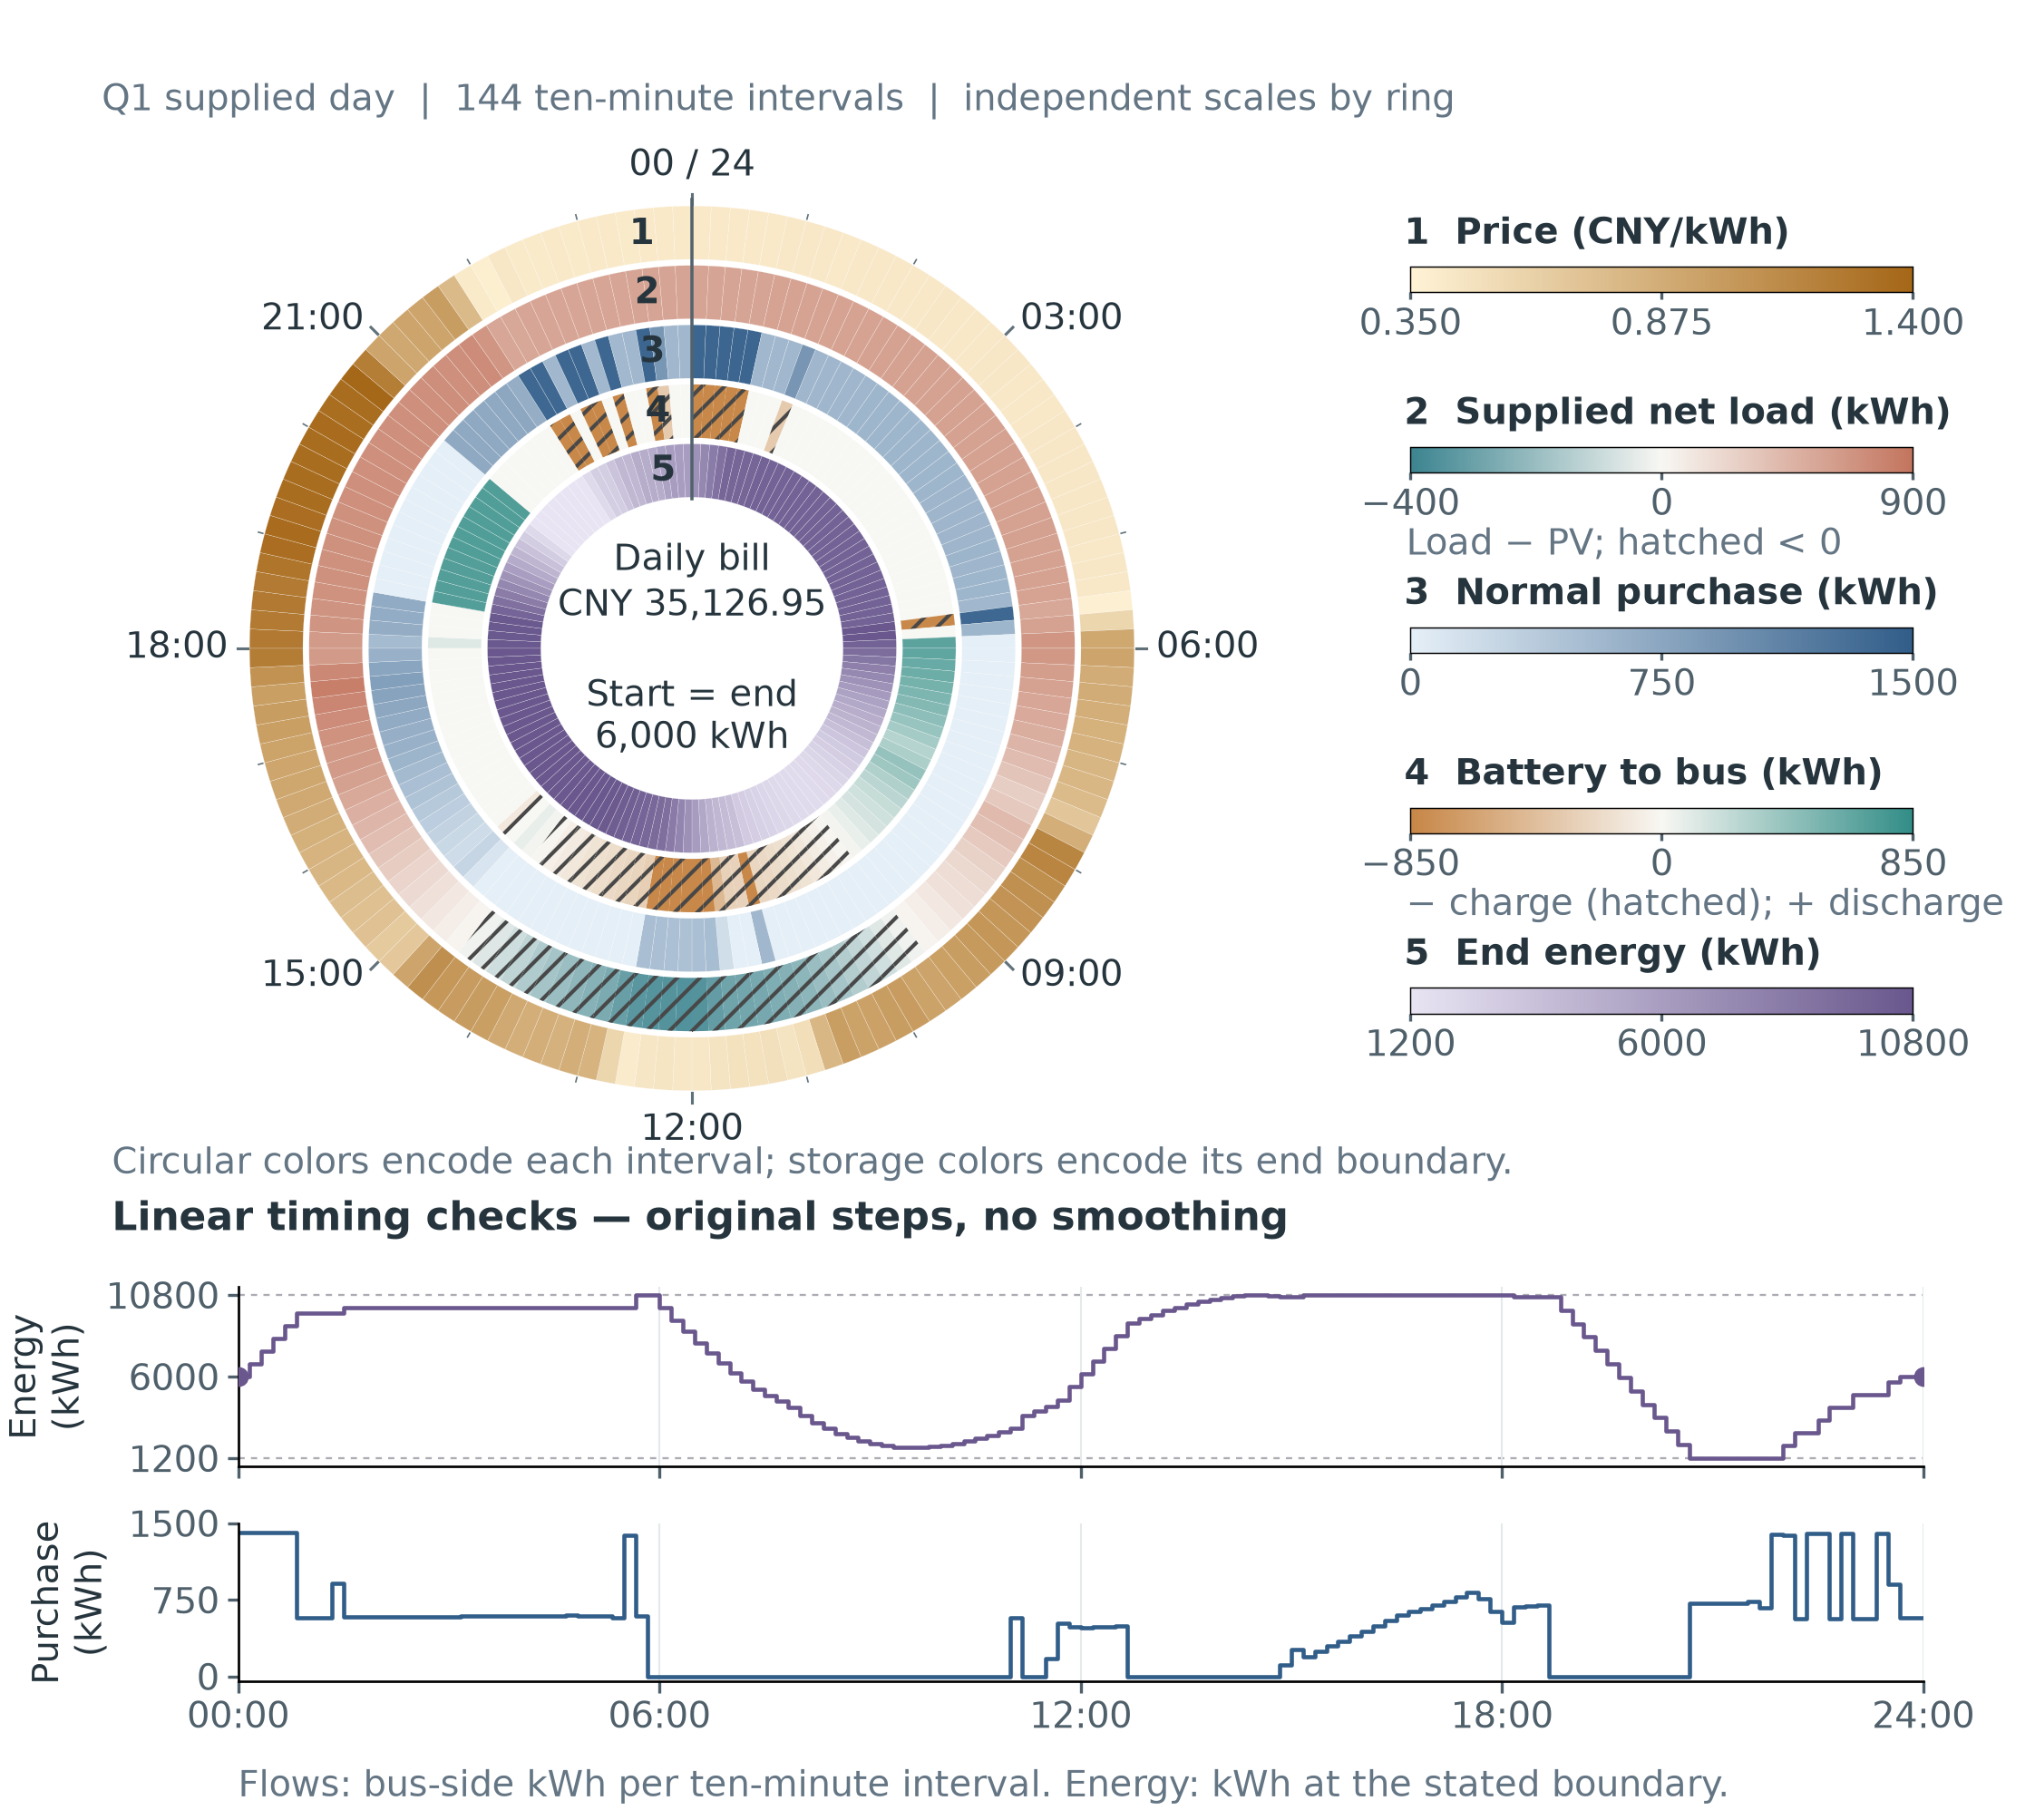
\includegraphics[width=\linewidth,height=150mm,keepaspectratio]{build/figure-04.png}
\caption{The saved Q1 schedule as a 24-hour circular matrix with linear step views. Each sector is one original ten-minute interval. Net load is load minus PV; battery exchange is bus-side discharge minus charge, positive for discharge. Independent scales distinguish price, interval energy, and stored energy. The storage ring uses interval-end energy; the linear trace retains all 145 boundaries from 00:00 to 24:00. Hatching marks negative values in the net-load and battery-flow rings.}
\label{fig:4}
\end{figure}

The returned energy trajectory reaches both the 1,200 and 10,800 kWh operating bounds while returning to 6,000 kWh at midnight. There are 45 charging intervals and 37 discharging intervals; 19 charging intervals attain the 5,000 kW bus limit. These counts describe this solution, not a unique operating pattern. A separately saved near-optimal alternative changes some purchases or states by up to 333.333333 kWh while changing cost by only \(10^{-7}\) CNY, showing that specific action times should not be interpreted as unique.

Tables 19-20 in Appendix D.1 give the prescribed Q1 outputs from \nolinkurl{result1.xlsx}; Table 18 maps each workbook to the statement requirements.

\subsection{Physical interpretation sensitivity and checks}\label{physical-interpretation-sensitivity-and-checks}

Two interpretations of the stated efficiency and two locations of the power rating yield the four existing deterministic cases in Table 6. In the battery-internal power case, bus flows are bounded by \(c_t\le P/\eta_c\) and \(b_t\le P\eta_d\); in the bus case each is bounded by \(P\).

% TABLE-BEGIN 6
\Needspace{95.6pt}
\begingroup
\fontsize{9.0}{10.8}\selectfont
\setlength{\tabcolsep}{3.2pt}
\renewcommand{\arraystretch}{1.12}
\setlength{\LTleft}{0pt plus 1fill}\setlength{\LTright}{0pt plus 1fill}
\setlength{\LTcapwidth}{\linewidth}

\begin{longtable}[]{@{}
  >{\raggedright\arraybackslash}p{(\linewidth - 4\tabcolsep) * \real{0.5126}}
  >{\raggedright\arraybackslash}p{(\linewidth - 4\tabcolsep) * \real{0.2701}}
  >{\raggedleft\arraybackslash}p{(\linewidth - 4\tabcolsep) * \real{0.2173}}@{}}
\caption{Q1 efficiency-by-power-side sensitivity.}\tabularnewline
\toprule\noalign{}
\begin{minipage}[b]{\linewidth}\raggedright
\textbf{Efficiency convention}
\end{minipage} & \begin{minipage}[b]{\linewidth}\raggedright
\textbf{Power rating applies at}
\end{minipage} & \begin{minipage}[b]{\linewidth}\raggedleft
\textbf{Cost (CNY)}
\end{minipage} \\
\midrule\noalign{}
\endfirsthead
\caption[]{Q1 efficiency-by-power-side sensitivity. (continued)}\tabularnewline
\toprule\noalign{}
\begin{minipage}[b]{\linewidth}\raggedright
\textbf{Efficiency convention}
\end{minipage} & \begin{minipage}[b]{\linewidth}\raggedright
\textbf{Power rating applies at}
\end{minipage} & \begin{minipage}[b]{\linewidth}\raggedleft
\textbf{Cost (CNY)}
\end{minipage} \\
\midrule\noalign{}
\endhead
\bottomrule\noalign{}
\endfoot
\bottomrule\noalign{}
\endlastfoot
0.9 in each direction & AC bus & 35,126.95 \\*
0.9 in each direction & Battery interior & 35,101.57 \\*
0.9 round trip, symmetric directions & AC bus & 33,801.50 \\*
0.9 round trip, symmetric directions & Battery interior & 33,790.32 \\*
\end{longtable}

\endgroup
% TABLE-END 6

The four MILPs and their same-builder LP relaxations agree in objective; 48 separate algebra checks verify the physical equations. The original baseline audit independently re-reads the saved schedule and source prices, with maximum balance residual \(1.14\times10^{-13}\) kWh and state-recursion residual \(8.81\times10^{-13}\) kWh, below the \(10^{-6}\) kWh threshold. It verifies fixed endpoints, mode exclusion, power limits, PV curtailment, and cost reconstruction. The LP comparison is useful numerical evidence, but is not an independently derived physical model. The sensitivity cases address the supplied day\textquotesingle s interpretation; no annual robustness conclusion follows from their differences.

A schedule optimized for forecast inputs can still leave expensive deficits when actual load and PV differ and normal purchases are fixed. Q2 therefore evaluates purchases by simulating execution under historical errors.

\section{Problem 2: History-Based Direct Procurement}\label{problem-2-history-based-direct-procurement}

\subsection{Forecast inputs and historical scenarios}\label{forecast-inputs-and-historical-scenarios}

Problem 2 requires a nonnegative vector of 144 purchases to be committed at midnight. The controller also chooses 144 discharge thresholds at midnight and holds them fixed for the day. Actual load, PV, and stored energy then determine discharge and emergency purchases through (3), while normal commitments remain payable. Under-purchasing can expose the microgrid to the fivefold emergency tariff; over-purchasing can leave paid energy unused. A reserve may avoid spending stored energy on an early low-price deficit, but it may also buy emergency energy unnecessarily. Purchases and this storage response must therefore be evaluated together.

\begingroup
\interlinepenalty=10000
\brokenpenalty=10000

We retain the causal forecasting structure selected during January as the common input to the procurement comparisons. This structure, denoted B0, combines a load regression with one-day and seven-day lags, weekday indicators and two daily harmonics, with a PV model using three daily harmonics and a bounded first-order residual adjustment. Load parameters use the preceding 28 eligible training days and PV parameters the preceding seven days; the residual coefficient is clipped to \([-0.99,0.99]\). The January 15-31 shadow comparison selected this structure using realized cost with an auxiliary terminal-inventory adjustment. Its structure was frozen on February 1, although parameters were subsequently re-estimated from available history. The seasonal comparator B1 uses the previous week\textquotesingle s load and previous day\textquotesingle s PV at the same time of day.

\par
\endgroup

That January choice did not retain its economic advantage over February-December. B0 incurred CNY 16,333,683.39, including CNY 4,345,851.83 of emergency cost, whereas B1 incurred CNY 15,378,207.35. B0 was CNY 955,476.04 more expensive. This is evidence about the complete forecast-and-purchase policies; it does not establish a ranking of their prediction errors. Keeping B0 fixed allows the subsequent procurement comparisons to use the same forecast input, without retrospectively replacing it in response to a new annual ranking. A stronger comparator first adds hourly historical net-error quantiles to the point forecast and then solves a deterministic procurement model. Its best retained profile uses quantiles 0.85 during 09:00-11:00, 0.65 during 11:00-18:00, 0.95 during 18:00-22:00 and 0.80 otherwise, estimated from the preceding 28 days. We call it the \emph{quantile-procurement baseline}. Its total cost is CNY 13,994,282.26 and emergency cost CNY 644,292.17. These are frozen historical references using their original execution and search procedures. Their nominal dispatch can differ from the greedy rule actually executed. The current paired experiment separately tests whether optimizing a discharge threshold helps under a matched search budget.

The Q2 branch of (5) uses the complete 144-interval B0 error vectors available at midnight, one shared \((q^0,R^0)\) pair, and current actual energy. It fixes both vectors for the day and has no final-energy equality. Algorithm 1 gives each controller twelve midnight candidates under matched search limits. Eligibility, within-day ordering, fee weights, and the distinction between nominal initialization and actual execution follow Section 3.

\subsection{Matched costs, selection, and historical variability}\label{matched-costs-selection-and-historical-variability}

The previous Q2 study selected \(W=112\), \(\kappa=5\), and \(\mu=0.38232\); its twelve-policy matrix remains historical evidence in Appendix B. Those values and the forecast model are fixed for this new experiment. The greedy and reserve arms each use four searches with identical per-search limits. Differences reflect the resulting controller/search procedures on separate continuous state paths, not a claim that the wider feasible policy class was globally optimized. The frozen D112 reference used two searches, so comparisons against it also include the changed search budget. Table 7 reports the matched Q2 costs and the two frozen references.

% TABLE-BEGIN 7
\Needspace{95.6pt}
\begingroup
\fontsize{9.0}{10.8}\selectfont
\setlength{\tabcolsep}{3.2pt}
\renewcommand{\arraystretch}{1.12}
\setlength{\LTleft}{0pt plus 1fill}\setlength{\LTright}{0pt plus 1fill}
\setlength{\LTcapwidth}{\linewidth}

\begin{longtable}[]{@{}
  >{\raggedright\arraybackslash}p{(\linewidth - 6\tabcolsep) * \real{0.3719}}
  >{\raggedleft\arraybackslash}p{(\linewidth - 6\tabcolsep) * \real{0.2253}}
  >{\raggedleft\arraybackslash}p{(\linewidth - 6\tabcolsep) * \real{0.1774}}
  >{\raggedleft\arraybackslash}p{(\linewidth - 6\tabcolsep) * \real{0.2253}}@{}}
\caption{Q2 matched controllers and frozen historical references, February-December 2025 (CNY).}\tabularnewline
\toprule\noalign{}
\begin{minipage}[b]{\linewidth}\raggedright
\textbf{Policy / controller}
\end{minipage} & \begin{minipage}[b]{\linewidth}\raggedleft
\textbf{Contract cost}
\end{minipage} & \begin{minipage}[b]{\linewidth}\raggedleft
\textbf{Emergency cost}
\end{minipage} & \begin{minipage}[b]{\linewidth}\raggedleft
\textbf{Total cost}
\end{minipage} \\
\midrule\noalign{}
\endfirsthead
\caption[]{Q2 matched controllers and frozen historical references, February-December 2025 (CNY). (continued)}\tabularnewline
\toprule\noalign{}
\begin{minipage}[b]{\linewidth}\raggedright
\textbf{Policy / controller}
\end{minipage} & \begin{minipage}[b]{\linewidth}\raggedleft
\textbf{Contract cost}
\end{minipage} & \begin{minipage}[b]{\linewidth}\raggedleft
\textbf{Emergency cost}
\end{minipage} & \begin{minipage}[b]{\linewidth}\raggedleft
\textbf{Total cost}
\end{minipage} \\
\midrule\noalign{}
\endhead
\bottomrule\noalign{}
\endfoot
\bottomrule\noalign{}
\endlastfoot
Frozen quantile baseline & 13,349,990.09 & 644,292.17 & 13,994,282.26 \\*
Frozen D112 (two searches) & 13,075,237.03 & 838,655.45 & 13,913,892.48 \\*
Matched greedy (four searches) & 13,075,508.77 & 839,452.30 & 13,914,961.06 \\*
Reserve (four searches) & 12,983,297.86 & 862,155.13 & 13,845,452.99 \\*
\end{longtable}

\endgroup
% TABLE-END 7

The reserve controller saves CNY 69,508.07 (0.500\%) against matched greedy. Ordinary commitments fall by CNY 92,210.91, while emergency fees rise by CNY 22,702.84. It purchases 20,865,128.06 kWh through normal commitments and 186,092.42 kWh through emergency purchases. Lower normal commitments therefore offset higher emergency expenditure. The one-million-CNY emergency reference in the earlier research served as a screening preference.

Q2\textquotesingle s prescribed-date results and emergency records are in Appendix D.2 (Tables 21-24) and \nolinkurl{result2.xlsx}.

\begin{figure}[!htbp]
\centering
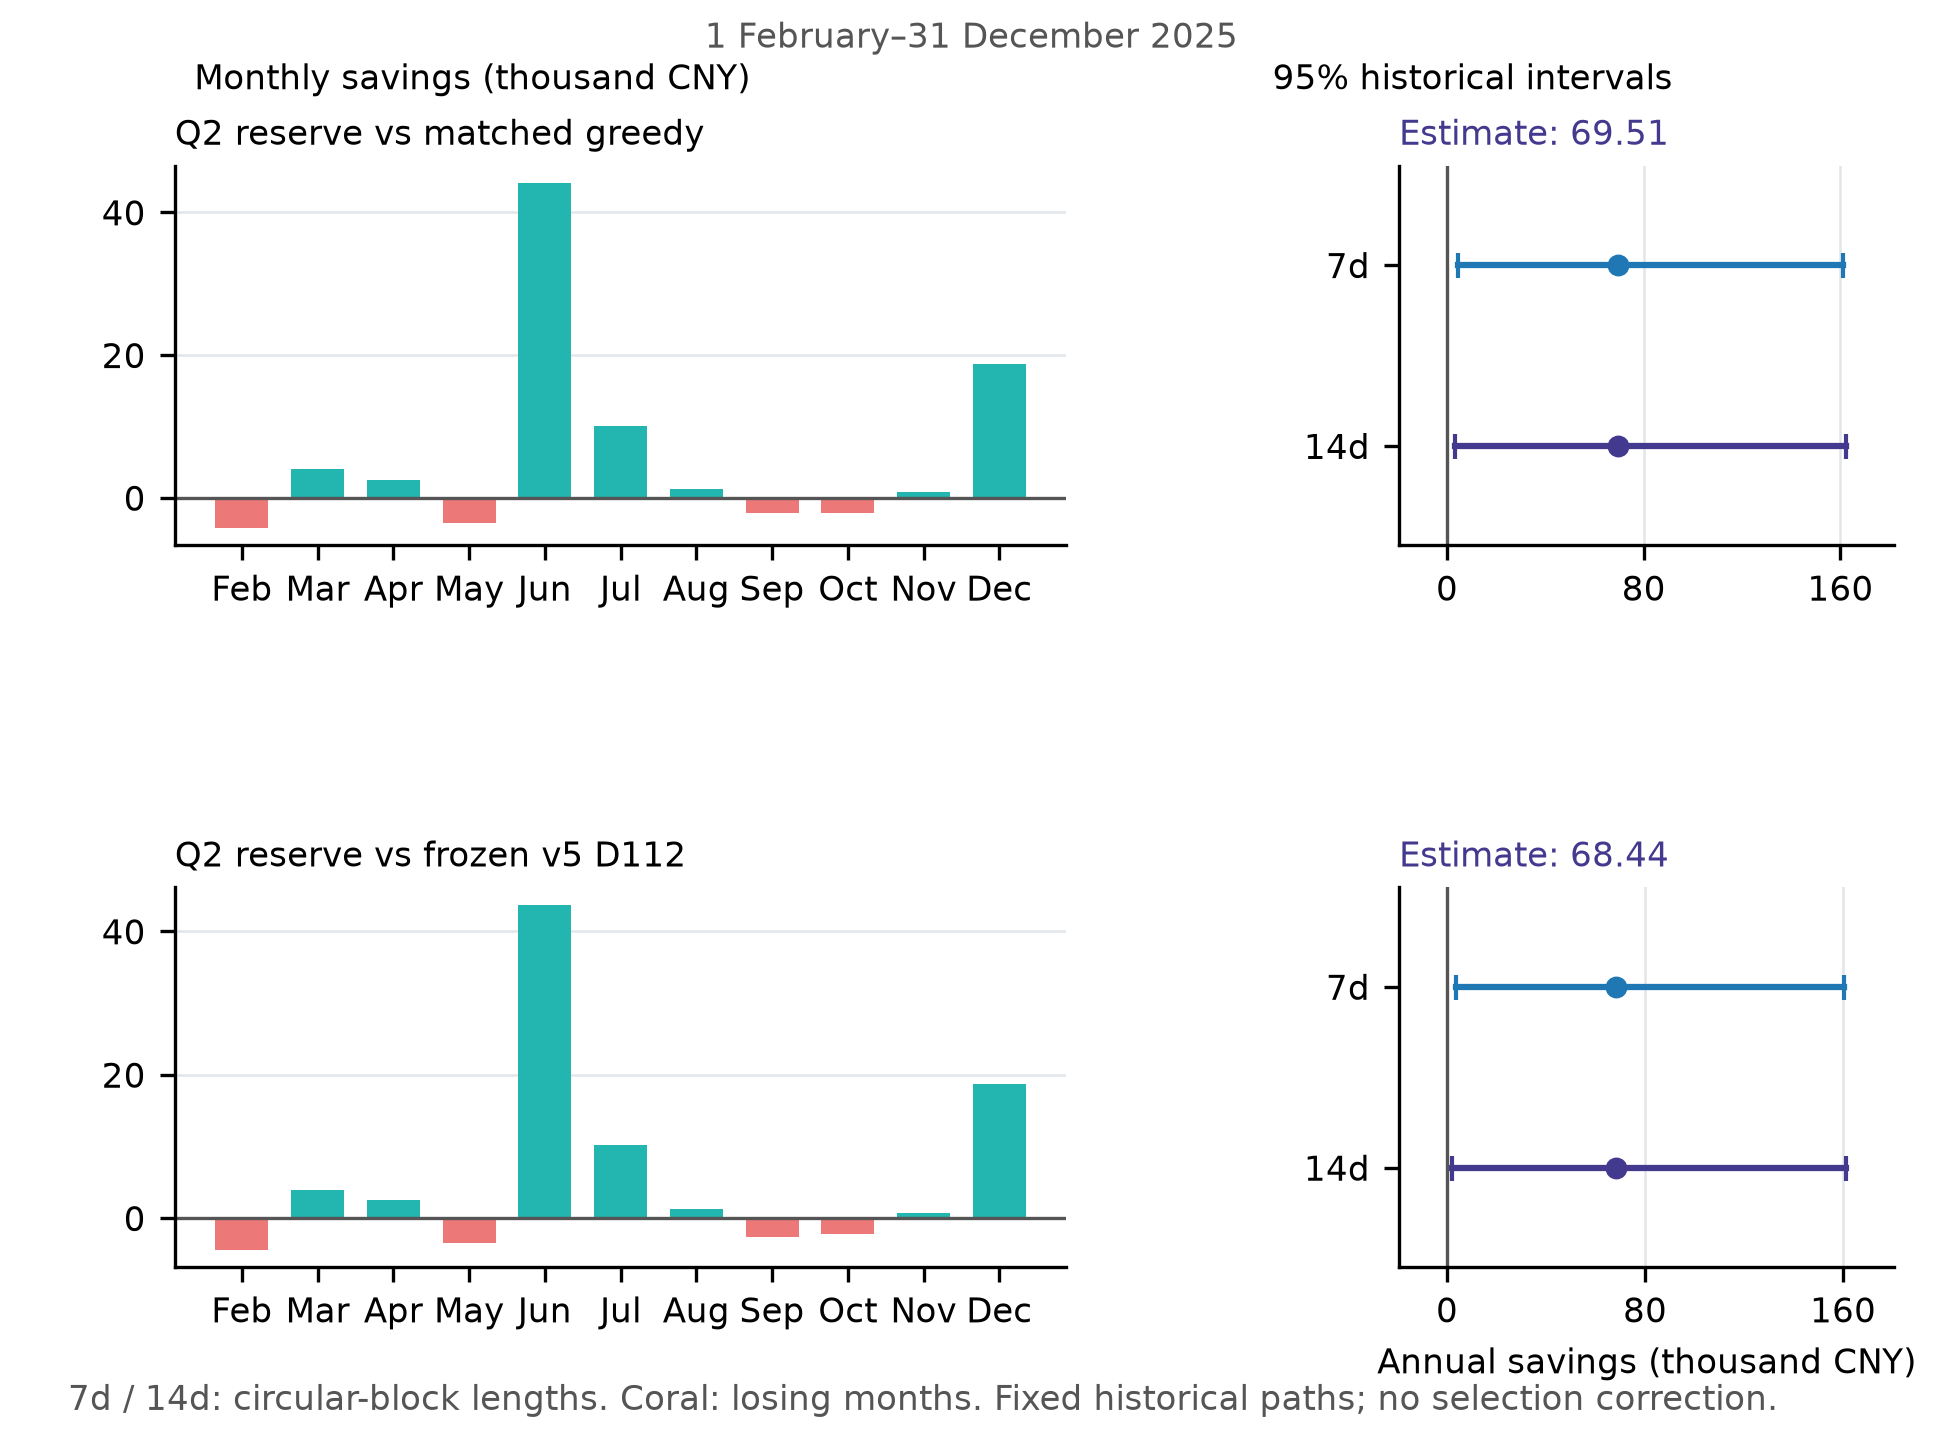
\includegraphics[width=\linewidth,height=150mm,keepaspectratio]{build/figure-05.png}
\caption{Q2 reserve-policy monthly savings and 7/14-day descriptive circular-block intervals against matched greedy and frozen D112 references. Negative months and any intervals crossing zero remain visible; the two references answer different comparison questions.}
\label{fig:5}
\end{figure}

Figure 5 shows the seasonal variation behind the annual saving: against matched greedy, Q2 wins on 221 days and loses on 113. Its 7-day interval is {[}4,484.52, 160,892.55{]} CNY; the 14-day interval is {[}3,279.77, 162,427.06{]} CNY. These resample fixed historical cost differences and do not generate new weather or battery paths. Section 8 reports the same convention across branches.

The maximum 112-day window contains 30-112 completed historical days: it is shorter during the first 82 evaluation days. Earlier changes to window length, inventory weight, emergency weight, and search limits are retained in Table 14 under their original greedy workflow. They motivated inherited settings but do not establish sensitivity or optimal parameter values for the new reserve controller. No annual retuning was performed in this experiment.

For scale, the preserved full-information reference has value CNY 12,227,565.30 under the common initial energy and equipment limits, free terminal energy within its bounds, and ordinary-priced total external supply. Its access to the whole future and relaxed supply price make it an idealized lower reference, not an implementable midnight policy. The current Q2 gap is CNY 1,617,887.69; it is not promised attainable saving or an estimated value of perfect information.

\section{Problem 3: Paid Rolling Procurement with Updated PV Forecasts}\label{problem-3-paid-rolling-procurement-with-updated-pv-forecasts}

\subsection{Rolling decisions and information comparisons}\label{rolling-decisions-and-information-comparisons}

\begingroup
\interlinepenalty=10000
\brokenpenalty=10000

Problem 3 adds forecasts released at 00:00, 06:00, 12:00 and 18:00 and permits paid procurement revisions after midnight. We retain Q2\textquotesingle s shared purchase/reserve objective, execution rule, and fixed parameters, using the current Attachment 3 forecast and the final-contract cost from Section 3. The load forecast is formed at midnight and remains fixed throughout the day. A PV release is interpolated onto the ten-minute grid and truncated at the current day\textquotesingle s midnight boundary. Although each release extends 24 hours ahead, this inherited optimization horizon ends at 24:00 of the present day.

\par
\endgroup

At release \(k\), only \((q_t^k,R_t^k)\) for \(t\in\mathcal T_k\) may change. Both executed vectors are frozen, and every scenario starts at actual energy \(E^{\mathrm{act}}_{d,\tau_k}\), not a previously forecast state. Historical errors match the PV release stage used at the current decision. Thus a noon update uses historical noon-issued PV errors, while an energy-feedback-only control retains the remaining portion of historical midnight errors. Reserve feedback does not relax these information cutoffs.

The contract term at midnight is \(p_tq^0_t\). At later releases it becomes \(F_A(q^k_t;q^0_t,p_t)\), always referenced to the original midnight quantity. Under this working settlement rule, an additional kWh above the original commitment costs \(1.5p_t\), while a reduction below it reduces the original bill by only \(0.5p_t\) per kWh. The candidate is evaluated with this remaining contract cost, scenario emergency cost and inventory proxy. Previously executed costs are sunk, and successive optimization objectives are never added to form the bill. Actual settlement applies \(F_A\) once to the final effective quantity \(\bar q_t\), plus the full \(5p_tu_t\) emergency charge.

These changes yield a rolling purchase/reserve policy. A remaining-horizon MILP uses the applicable contract objective to supply a risk-profile purchase start and nominal energy values for one reserve start. Its optimized dispatch is not the final execution policy. Final decisions impose no daily terminal-energy equality, and actual energy follows (3) continuously across days and months.

At midnight, four searches generate twelve candidate pairs and the selected pair becomes \((q^0,R^0)\). At 06:00, 12:00 and 18:00, the current pair of future purchase and reserve vectors is retained as candidate thirteen. Retaining it avoids forcing a search result with a worse current empirical score, but cannot assure a lower later realized bill. An opportunity may change purchases, thresholds, both, or neither; unchanged purchases alone do not mean the controller took no action.

Within each controller family, the no-update policy retains the midnight PV and both decisions all day. The state-feedback policy may revise future purchases and thresholds from actual energy but retains the midnight PV release. The raw-PV policy also uses subsequent forecast releases. All begin at the same February initial energy; later states develop independently as consequences of the policies. Contract cost includes the final adjustment against the original commitment and excludes emergencies.

\begin{figure}[!htbp]
\centering
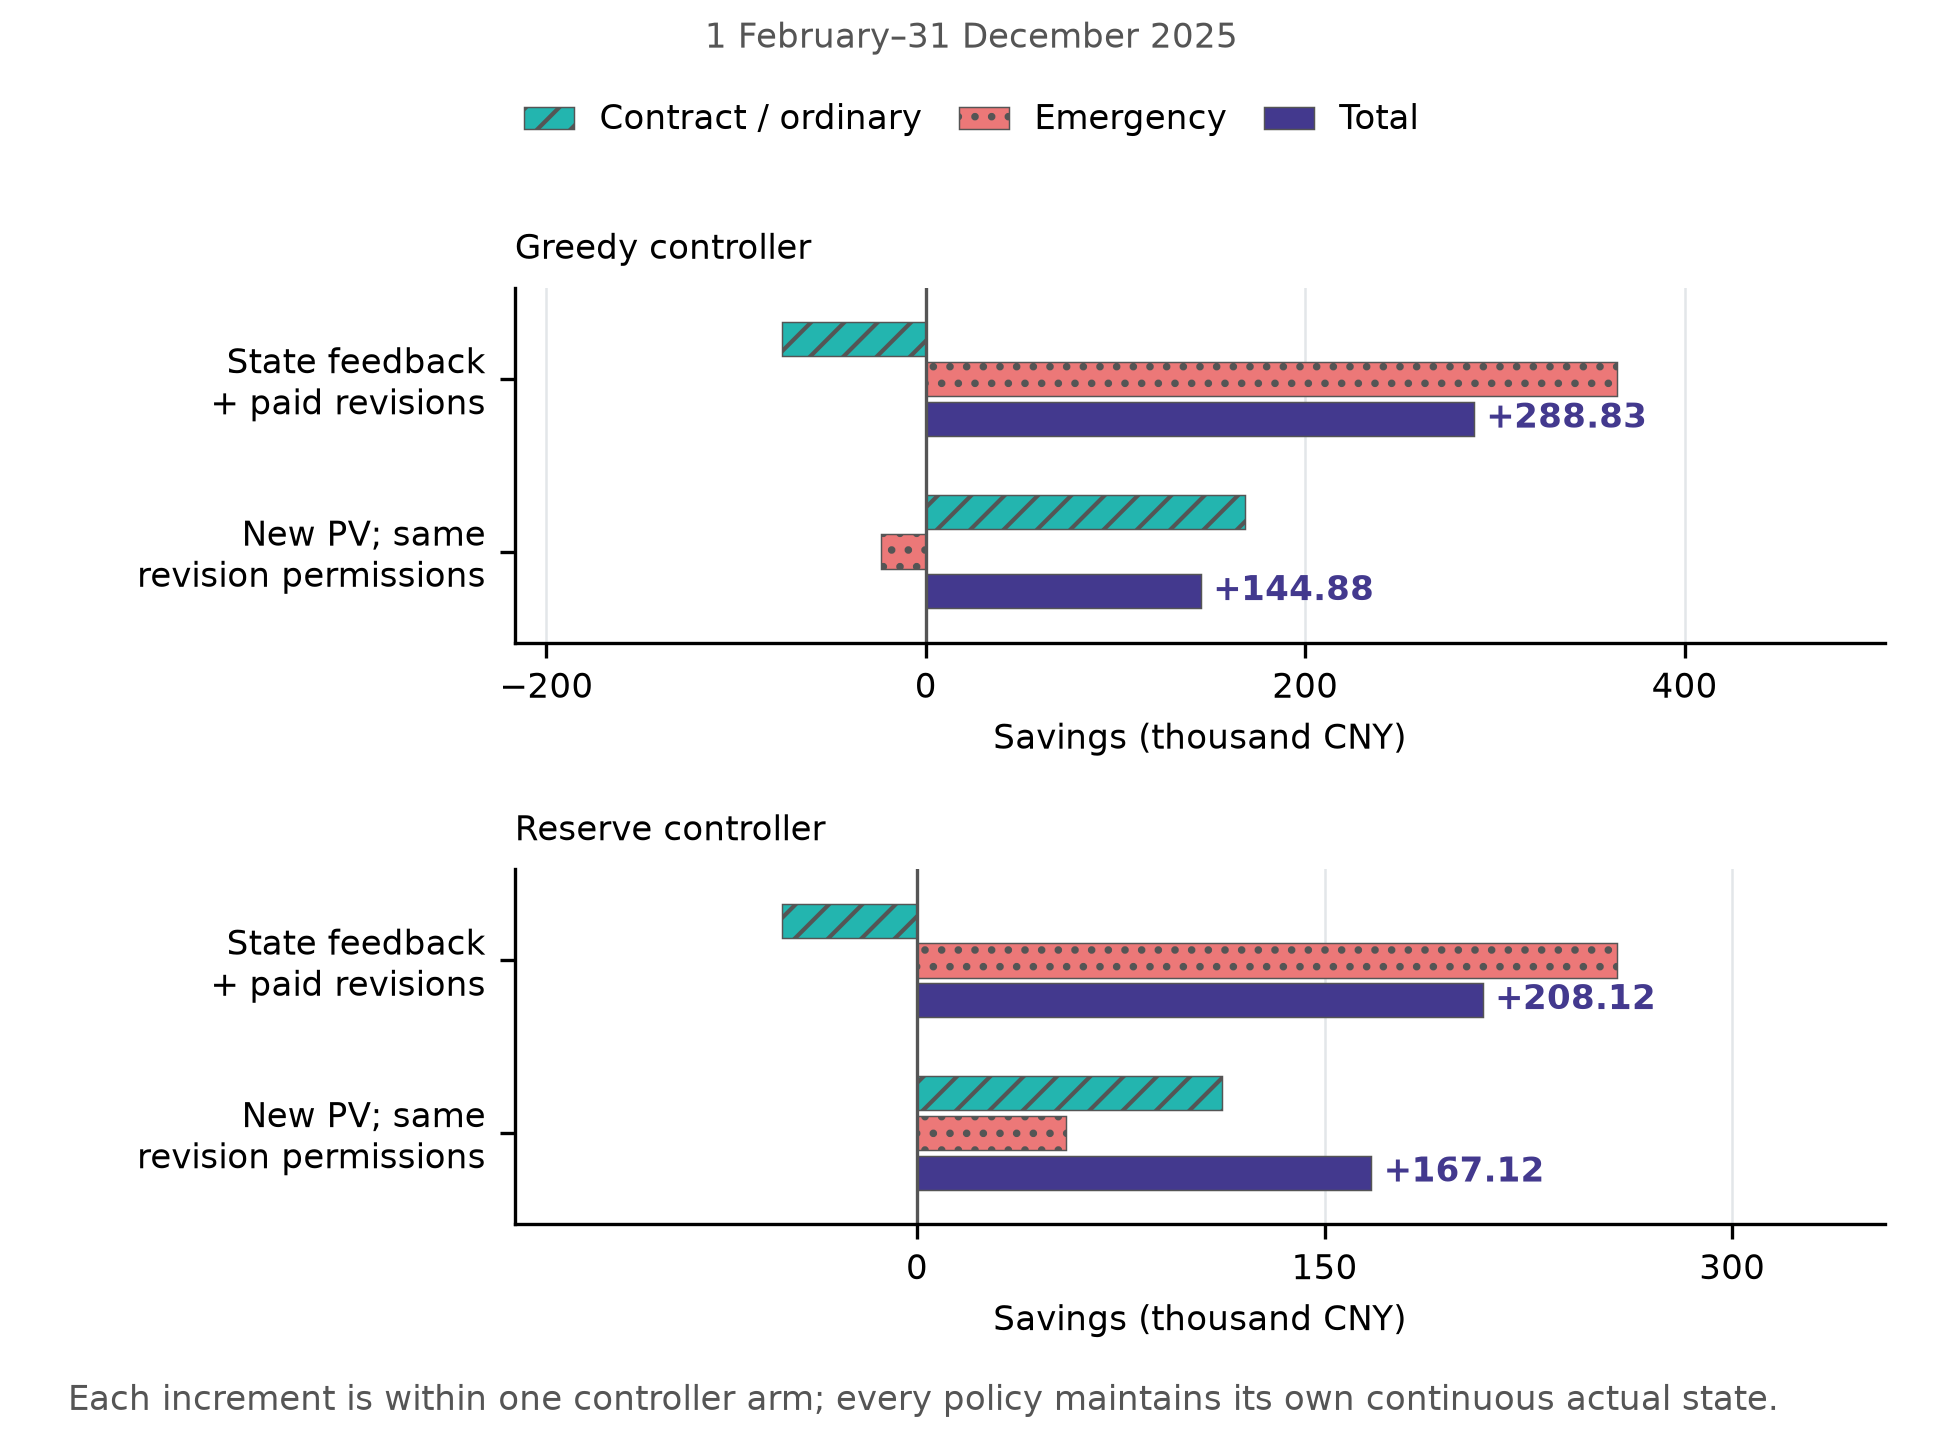
\includegraphics[width=\linewidth,height=150mm,keepaspectratio]{build/figure-06.png}
\caption{Q3 information comparisons within each storage-controller family. Signed contract and emergency savings distinguish state feedback with revisions from the additional effect of later raw PV releases. Each comparison uses 334 matched dates.}
\label{fig:6}
\end{figure}

Figure 6 separates the savings associated with state feedback and later PV releases. In the reserve family, state feedback with paid revisions saves CNY 208,115.60. Its contract saving is CNY -49,627.38 and emergency saving CNY 257,742.98. Adding later raw PV releases saves CNY 167,121.93, with contract and emergency savings of CNY 112,167.65 and 54,954.28. The combined raw-PV change saves CNY 375,237.53. Negative components denote higher expenditure.

\begingroup
\interlinepenalty=10000
\brokenpenalty=10000

The first difference combines observed-state feedback and revision permission. The second isolates the policy effect of later PV releases under the same permissions, including subsequent state changes. Neither estimates a universal price for information or the contribution of one particular release. Table 15 retains greedy controls so these effects are not inferred by comparing different storage rules.

\par
\endgroup

\subsection{Correction and the selected policy\textquotesingle s negative result}\label{correction-and-the-selected-policys-negative-result}

Persistent forecast bias motivates testing a correction, but its value must be judged through the purchasing decision. We retain the existing 28-day correction as a candidate. The correction is fitted and applied to the interpolated ten-minute energy forecasts (kWh). For each release hour, it estimates the mean actual-minus-raw-PV error from eligible positive raw forecasts whose target intervals are within the previous 28 days and have ended by the current day\textquotesingle s midnight. It uses only targets belonging to the historical release day. The same-day observations between midnight and a later release do not enter this correction fit. A positive raw forecast receives the estimated bias and is clipped at zero; an originally zero forecast remains zero.

The deployment rule activates the correction on April 1; February and March use raw PV. Historical scenario errors are reconstructed using each historical day\textquotesingle s own deployable forecast and bias parameters. We do not apply today\textquotesingle s correction retrospectively to older predictions. A window spanning April 1 therefore contains the original and corrected forecast versions actually prescribed on their respective dates. This preserves the deployment record while leaving a documented nonstationarity in the residual pool.

% TABLE-BEGIN 8
\Needspace{85.0pt}
\begingroup
\fontsize{9.0}{10.8}\selectfont
\setlength{\tabcolsep}{3.2pt}
\renewcommand{\arraystretch}{1.12}
\setlength{\LTleft}{0pt plus 1fill}\setlength{\LTright}{0pt plus 1fill}
\setlength{\LTcapwidth}{\linewidth}

\begin{longtable}[]{@{}
  >{\raggedright\arraybackslash}p{(\linewidth - 6\tabcolsep) * \real{0.2391}}
  >{\raggedleft\arraybackslash}p{(\linewidth - 6\tabcolsep) * \real{0.2761}}
  >{\raggedleft\arraybackslash}p{(\linewidth - 6\tabcolsep) * \real{0.2761}}
  >{\raggedleft\arraybackslash}p{(\linewidth - 6\tabcolsep) * \real{0.2087}}@{}}
\caption{Q3 PV correction in each matched controller, 334 days (CNY).}\tabularnewline
\toprule\noalign{}
\begin{minipage}[b]{\linewidth}\raggedright
\textbf{Controller}
\end{minipage} & \begin{minipage}[b]{\linewidth}\raggedleft
\textbf{Raw PV}
\end{minipage} & \begin{minipage}[b]{\linewidth}\raggedleft
\textbf{Correction from April 1}
\end{minipage} & \begin{minipage}[b]{\linewidth}\raggedleft
\textbf{Saving from correction}
\end{minipage} \\
\midrule\noalign{}
\endfirsthead
\caption[]{Q3 PV correction in each matched controller, 334 days (CNY). (continued)}\tabularnewline
\toprule\noalign{}
\begin{minipage}[b]{\linewidth}\raggedright
\textbf{Controller}
\end{minipage} & \begin{minipage}[b]{\linewidth}\raggedleft
\textbf{Raw PV}
\end{minipage} & \begin{minipage}[b]{\linewidth}\raggedleft
\textbf{Correction from April 1}
\end{minipage} & \begin{minipage}[b]{\linewidth}\raggedleft
\textbf{Saving from correction}
\end{minipage} \\
\midrule\noalign{}
\endhead
\bottomrule\noalign{}
\endfoot
\bottomrule\noalign{}
\endlastfoot
Greedy & 13,559,330.38 & 13,568,255.74 & -8,925.36 \\*
Reserve & 13,574,997.43 & 13,574,461.81 & 535.62 \\*
\end{longtable}

\endgroup
% TABLE-END 8

Q3 correction saves CNY 535.62 in the reserve arm and costs an additional CNY 8,925.36 in the greedy arm. This reversal ties the correction\textquotesingle s value to the full purchasing and storage procedure. The earlier nominal-MILP correction study uses a different purchasing method (Appendix B).

The reserve correction wins on 121 days, loses on 154, and ties on 59. Its 7-day interval is {[}-25,199.40, 28,640.66{]} CNY and its 14-day interval {[}-26,491.00, 29,134.66{]} CNY. Both cross zero. The corrected choice follows unrounded historical cash ranking, without establishing a stable correction benefit; these are correction comparisons, distinct from the controller comparisons in Section 8.

The submission retains reserve-family selection as its declared study scope, with historical cash cost ranking the PV variants within that family. Greedy policies remain economic controls in the full comparison. Under this restriction, the submitted Q3 schedule is not the least-cost policy across both families.

The reserve-family selection is \nolinkurl{q3_w28_reserve}, the corrected-PV rolling reserve policy. Original commitments cost CNY 13,276,739.67; upward and downward terms are CNY 208,355.49 and -250,200.37. Together, these terms give a contract bill of CNY 13,234,894.79. Adding CNY 339,567.02 of emergencies gives CNY 13,574,461.81. The final effective quantities are settled once, rather than summing all issued versions.

Against the same input configuration with matched greedy control, this policy costs an additional CNY 6,206.07. Thus the Q3 comparison provides no realized cash advantage for the added reserve control. Possible contributors include finite search, differences between historical scenarios and realized conditions, and their effects on later storage states; their separate contributions were not isolated. Table 15 reports all eight Q3 outcomes.

The selected Q3 schedule is detailed in Appendix D.3, Tables 25-28, and \nolinkurl{result3.xlsx}, including its original and revised purchases.

\section{Problem 4: Planning Prices and Realized Variable-Price Settlement}\label{problem-4-planning-prices-and-realized-variable-price-settlement}

\subsection{Price information without advance knowledge of actual tariffs}\label{price-information-without-advance-knowledge-of-actual-tariffs}

Attachment 4 records realized prices but does not state that a complete future price path is available when purchases are decided. We therefore compare two implementable planning inputs: the known fixed tariff from Attachment 1 and a causal price forecast. In both cases, the actual bill uses Attachment 4 prices for the target intervals. Using a fixed reference in the optimizer defines a purchasing rule under uncertain prices; settlement still uses the actual tariff.

\Needspace{14\baselineskip}

The causal forecast uses ordinary least squares with a trailing 28-calendar-day window. Its predictors are an intercept, two daily Fourier harmonics, one-day and seven-day price lags, and six weekday indicators. Writing \(\phi_t\) for the fraction of the day elapsed at interval \(t\), the planning price is

\[
\begin{aligned}
\widetilde p_{d,t\mid k}
&=\beta_0+\sum_{j=1}^{2}\left[a_j\sin(2\pi j\phi_t)+b_j\cos(2\pi j\phi_t)\right]\\
&\quad+\beta_1p^{\mathrm{act}}_{d-1,t}+\beta_7p^{\mathrm{act}}_{d-7,t}
+\sum_{r=1}^{6}\gamma_r\mathbf1\{\mathrm{weekday}(d)=r\},\\
p^{\mathrm{plan}}_{d,t\mid k}&=\max\{10^{-6},\widetilde p_{d,t\mid k}\}.
\end{aligned} \tag{10}
\]

Coefficients are re-estimated at each allowed decision time using only completed price observations. Equivalently, with the 13-column design matrix \(X\) and observed training-price vector \(y\) at the current issue, the fit minimizes \(\|X\theta-y\|_2^2\) over \(\theta\in\mathbb R^{13}\); it adds no procurement constraint. Training rows must also have their lagged predictors available. Since the prediction horizon ends at the current day\textquotesingle s 24:00, its previous-day and previous-week lags are already observed. At an intraday decision, completed current-day prices may enter the training window, while uncompleted and future target prices cannot. The floor of \(10^{-6}\) CNY/kWh is a fixed numerical positivity rule, not a minimum estimated from the evaluation period. This regression supplies decision inputs; correlated ten-minute observations are not treated as independent samples for coefficient-significance claims.

We interpret recalculating Problem 2 under variable prices as retaining its historical-PV information set. The statement lists Attachments 2-4 for Problem 4 without an explicit branch-specific ban on Attachment 3; the Q4-2 boundary in Table 3 is therefore a working interpretation. Under it, Q4-2 uses B0 load and historical-PV forecasts, excludes Attachment 3, and fixes both its 144 purchases and 144 reserve thresholds at midnight. Q4-3 uses the available Attachment 3 releases and actual energy feedback, with future purchase/reserve updates at 06:00, 12:00 and 18:00. Both inherit \(W=112\), \(\kappa=5\), \(\mu=0.38232\), the four-search protocol, and physical parameters without retuning. The planning price enters both ordinary contract cost and scenario emergency cost in (5), so it can alter procurement and the timing of energy retention. Changing only the ordinary-price term while keeping emergency weights at fixed tariffs would not implement this comparison.

During execution, \(p^{\mathrm{act}}\) determines cash settlement for normal purchases, contract adjustments, and emergencies. It does not replace a preissued threshold using information that was unavailable when that threshold was chosen. The inherited inventory coefficient remains a planning proxy and is never deducted from the bill. Planning prices influence the selected \((q,R)\) pair; realized prices determine its cash cost.

\subsection{Price comparisons and selected policies}\label{price-comparisons-and-selected-policies}

Table 15 compares fixed-reference and causal-OLS planning prices within each controller. Actual settlement, information access, physical limits, initialization, and search settings are held fixed. This comparison does not add Attachment 3 to the midnight branch.

OLS saves CNY 3,079.27 in the reserve family and costs an additional CNY 6,786.91 in the matched greedy family. The selected reserve policy is \nolinkurl{q42_ols_reserve}. Its total CNY 14,618,518.98 comprises CNY 13,704,872.50 of ordinary fees and CNY 913,646.48 of emergencies, all at actual variable prices. The selected policy saves CNY 68,043.65 relative to its same-input greedy control.

For OLS versus fixed planning prices within the reserve family, the 7-day interval is {[}-31,696.16, 32,765.14{]} CNY and the 14-day interval {[}-32,148.32, 34,023.98{]} CNY. Both cross zero. They describe the price-input ranking and are not replaced by the reserve-versus-greedy intervals in Table 10.

For each controller, Q2 and the fixed-planning-price Q4-2 policy produce identical purchases, thresholds, and physical paths. Their cash bills differ because Q4-2 uses Attachment 4 actual prices. The independent comparison checks this identity for all 48,096 intervals and both arms; a different physical path here would indicate an unintended planning change.

Appendix D.4, Tables 29-32, and \nolinkurl{result4-2.xlsx} contain the prescribed-date outputs for the selected Q4-2 policy.

\begin{figure}[!htbp]
\centering
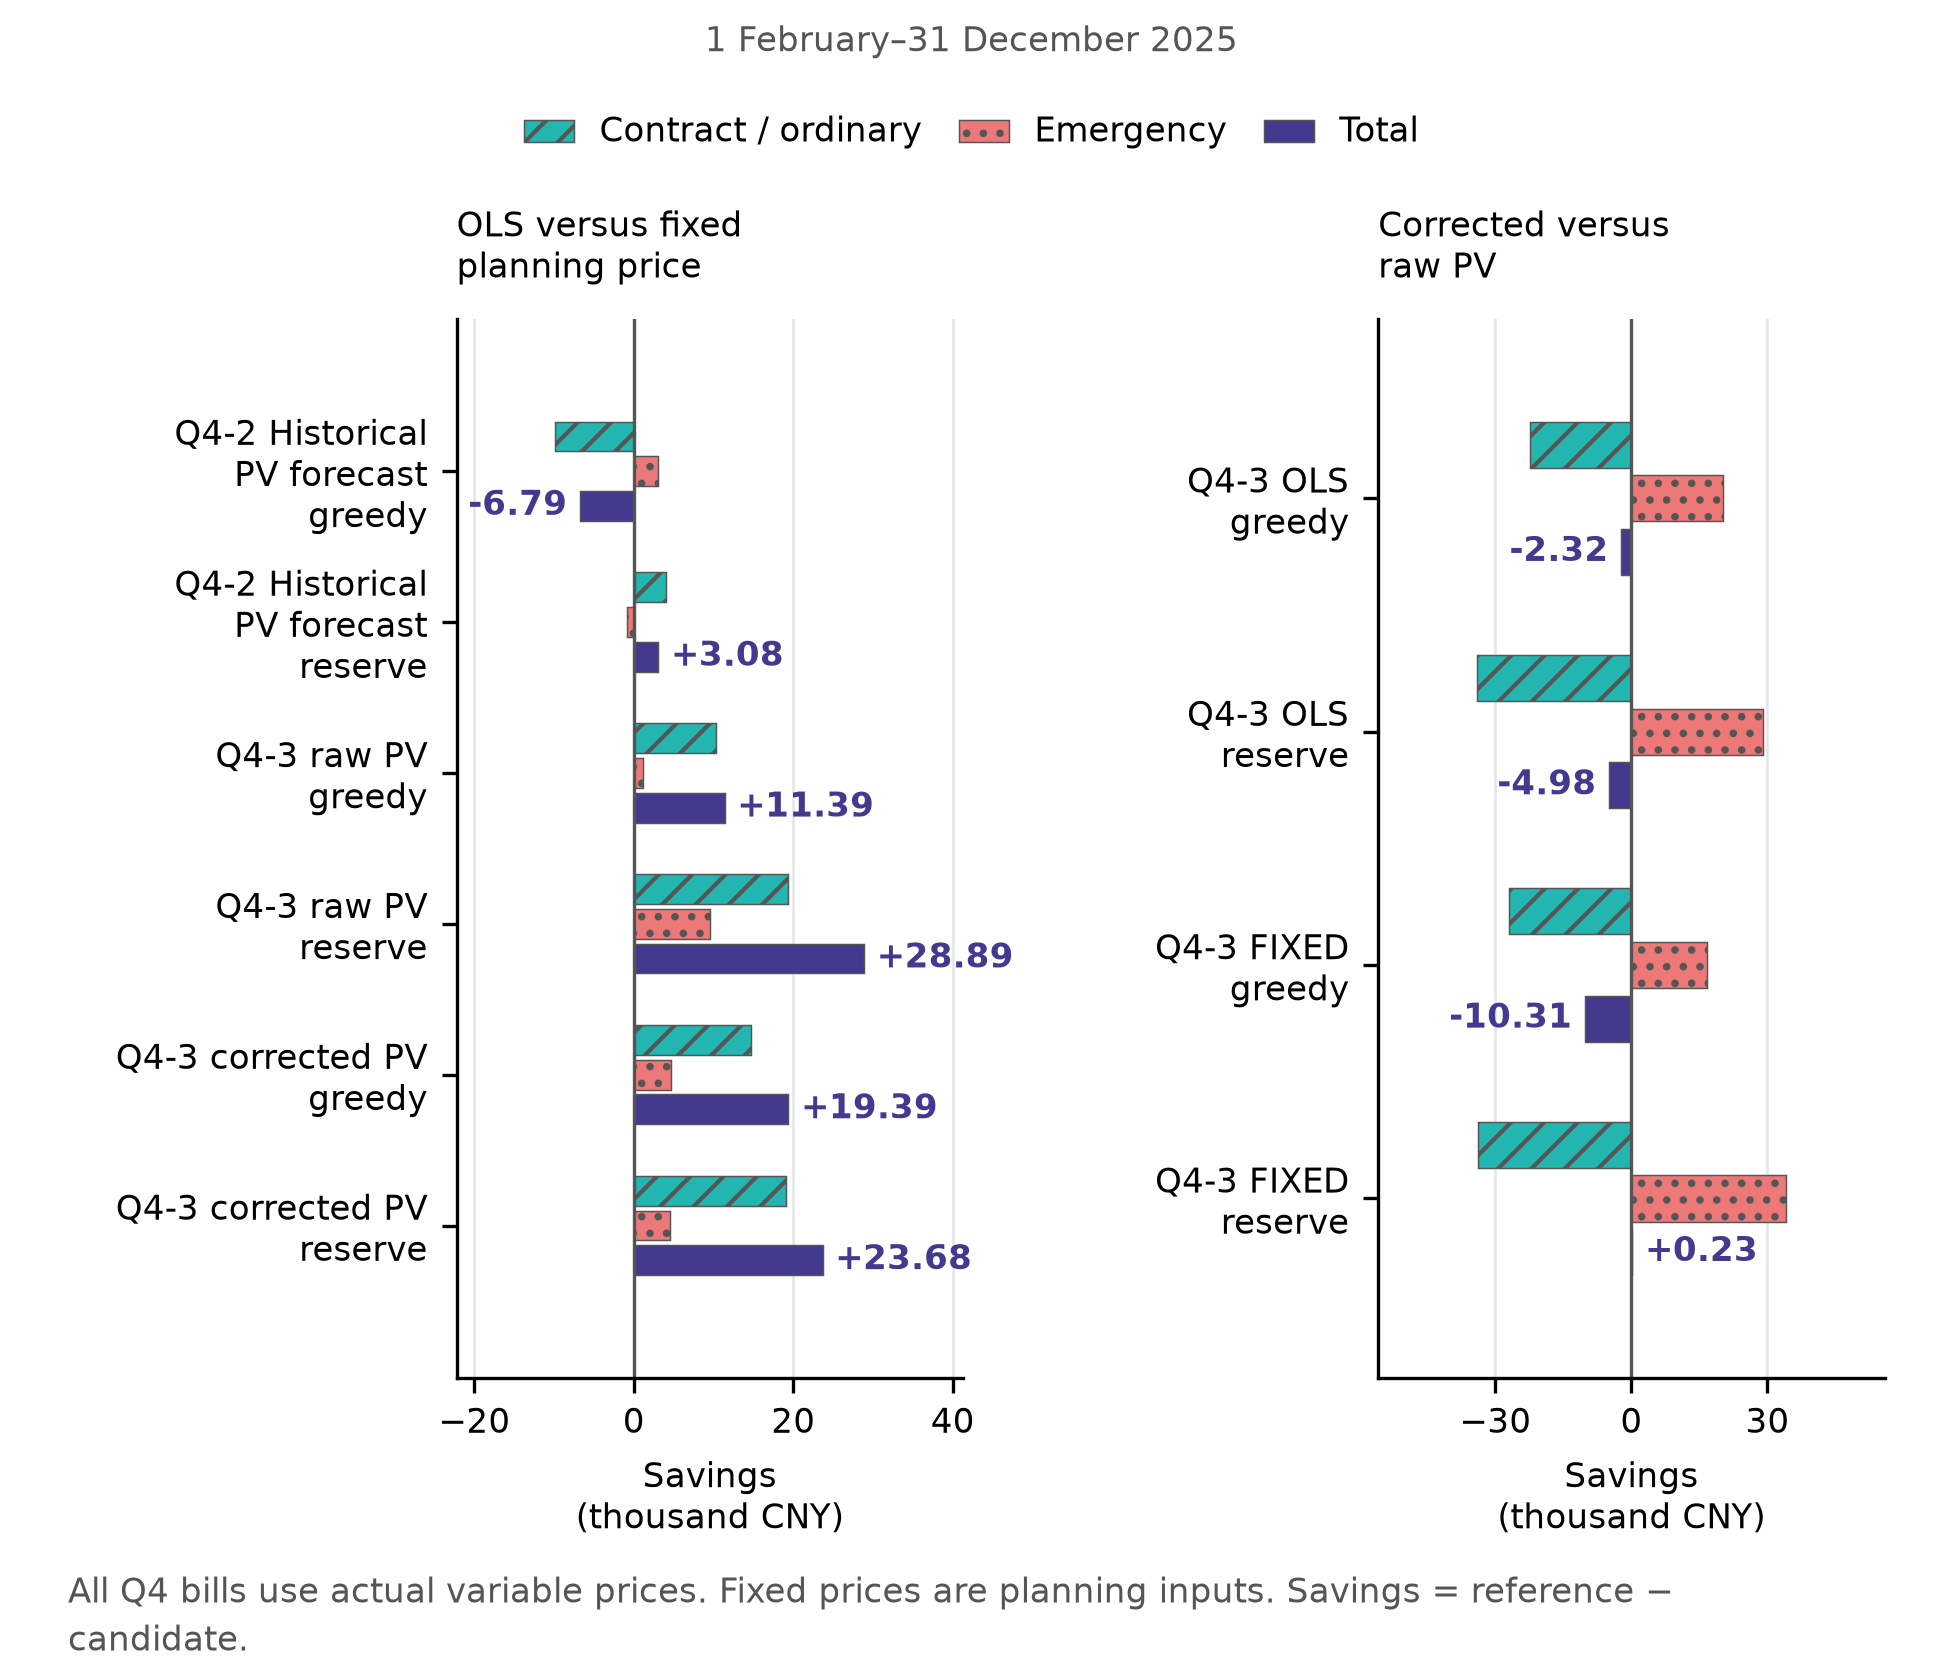
\includegraphics[width=\linewidth,height=150mm,keepaspectratio]{build/figure-07.png}
\caption{Q4 planning-price and PV-correction comparisons under matched storage controllers. Q4-2 retains historical PV; Q4-3 uses the permitted forecast releases. Every cost is billed at actual variable prices, regardless of its planning-price input.}
\label{fig:7}
\end{figure}

Figure 7 compares the price and PV-correction choices. With raw PV, causal OLS saves CNY 28,892.88 in the reserve arm. Under OLS, PV correction costs an additional CNY 4,984.88; under fixed planning prices it saves CNY 230.32. The selected reserve policy is \nolinkurl{q43_raw_ols_reserve}, the raw-PV/causal-OLS rolling reserve policy. It saves CNY 7,194.43 against the matched greedy configuration. Table 15 preserves all eight outcomes so price effects are not inferred from differently corrected PV inputs or controllers.

The raw-PV OLS-versus-fixed comparison has positive descriptive intervals: {[}14,140.65, 44,563.84{]} CNY with 7-day blocks and {[}11,797.92, 46,451.05{]} CNY with 14-day blocks. In contrast, both block lengths cross zero for each reserve-family PV-correction comparison, under fixed and OLS planning prices. These intervals distinguish the observed price effect from the smaller correction rankings; Section 8 defines their resampling scope.

The corresponding Q4-3 outputs, including paid revisions and emergency events, are in Appendix D.5, Tables 33-36, and \nolinkurl{result4-3.xlsx}.

Figure 8 uses the prespecified diagnostic date, 14 July 2025, to show how released planning prices and procurement versions lead to the executed energy and reserve trace. Each version starts at its release and leaves completed intervals fixed. The actual-price trace provides retrospective settlement context.

\begin{figure}[!htbp]
\centering
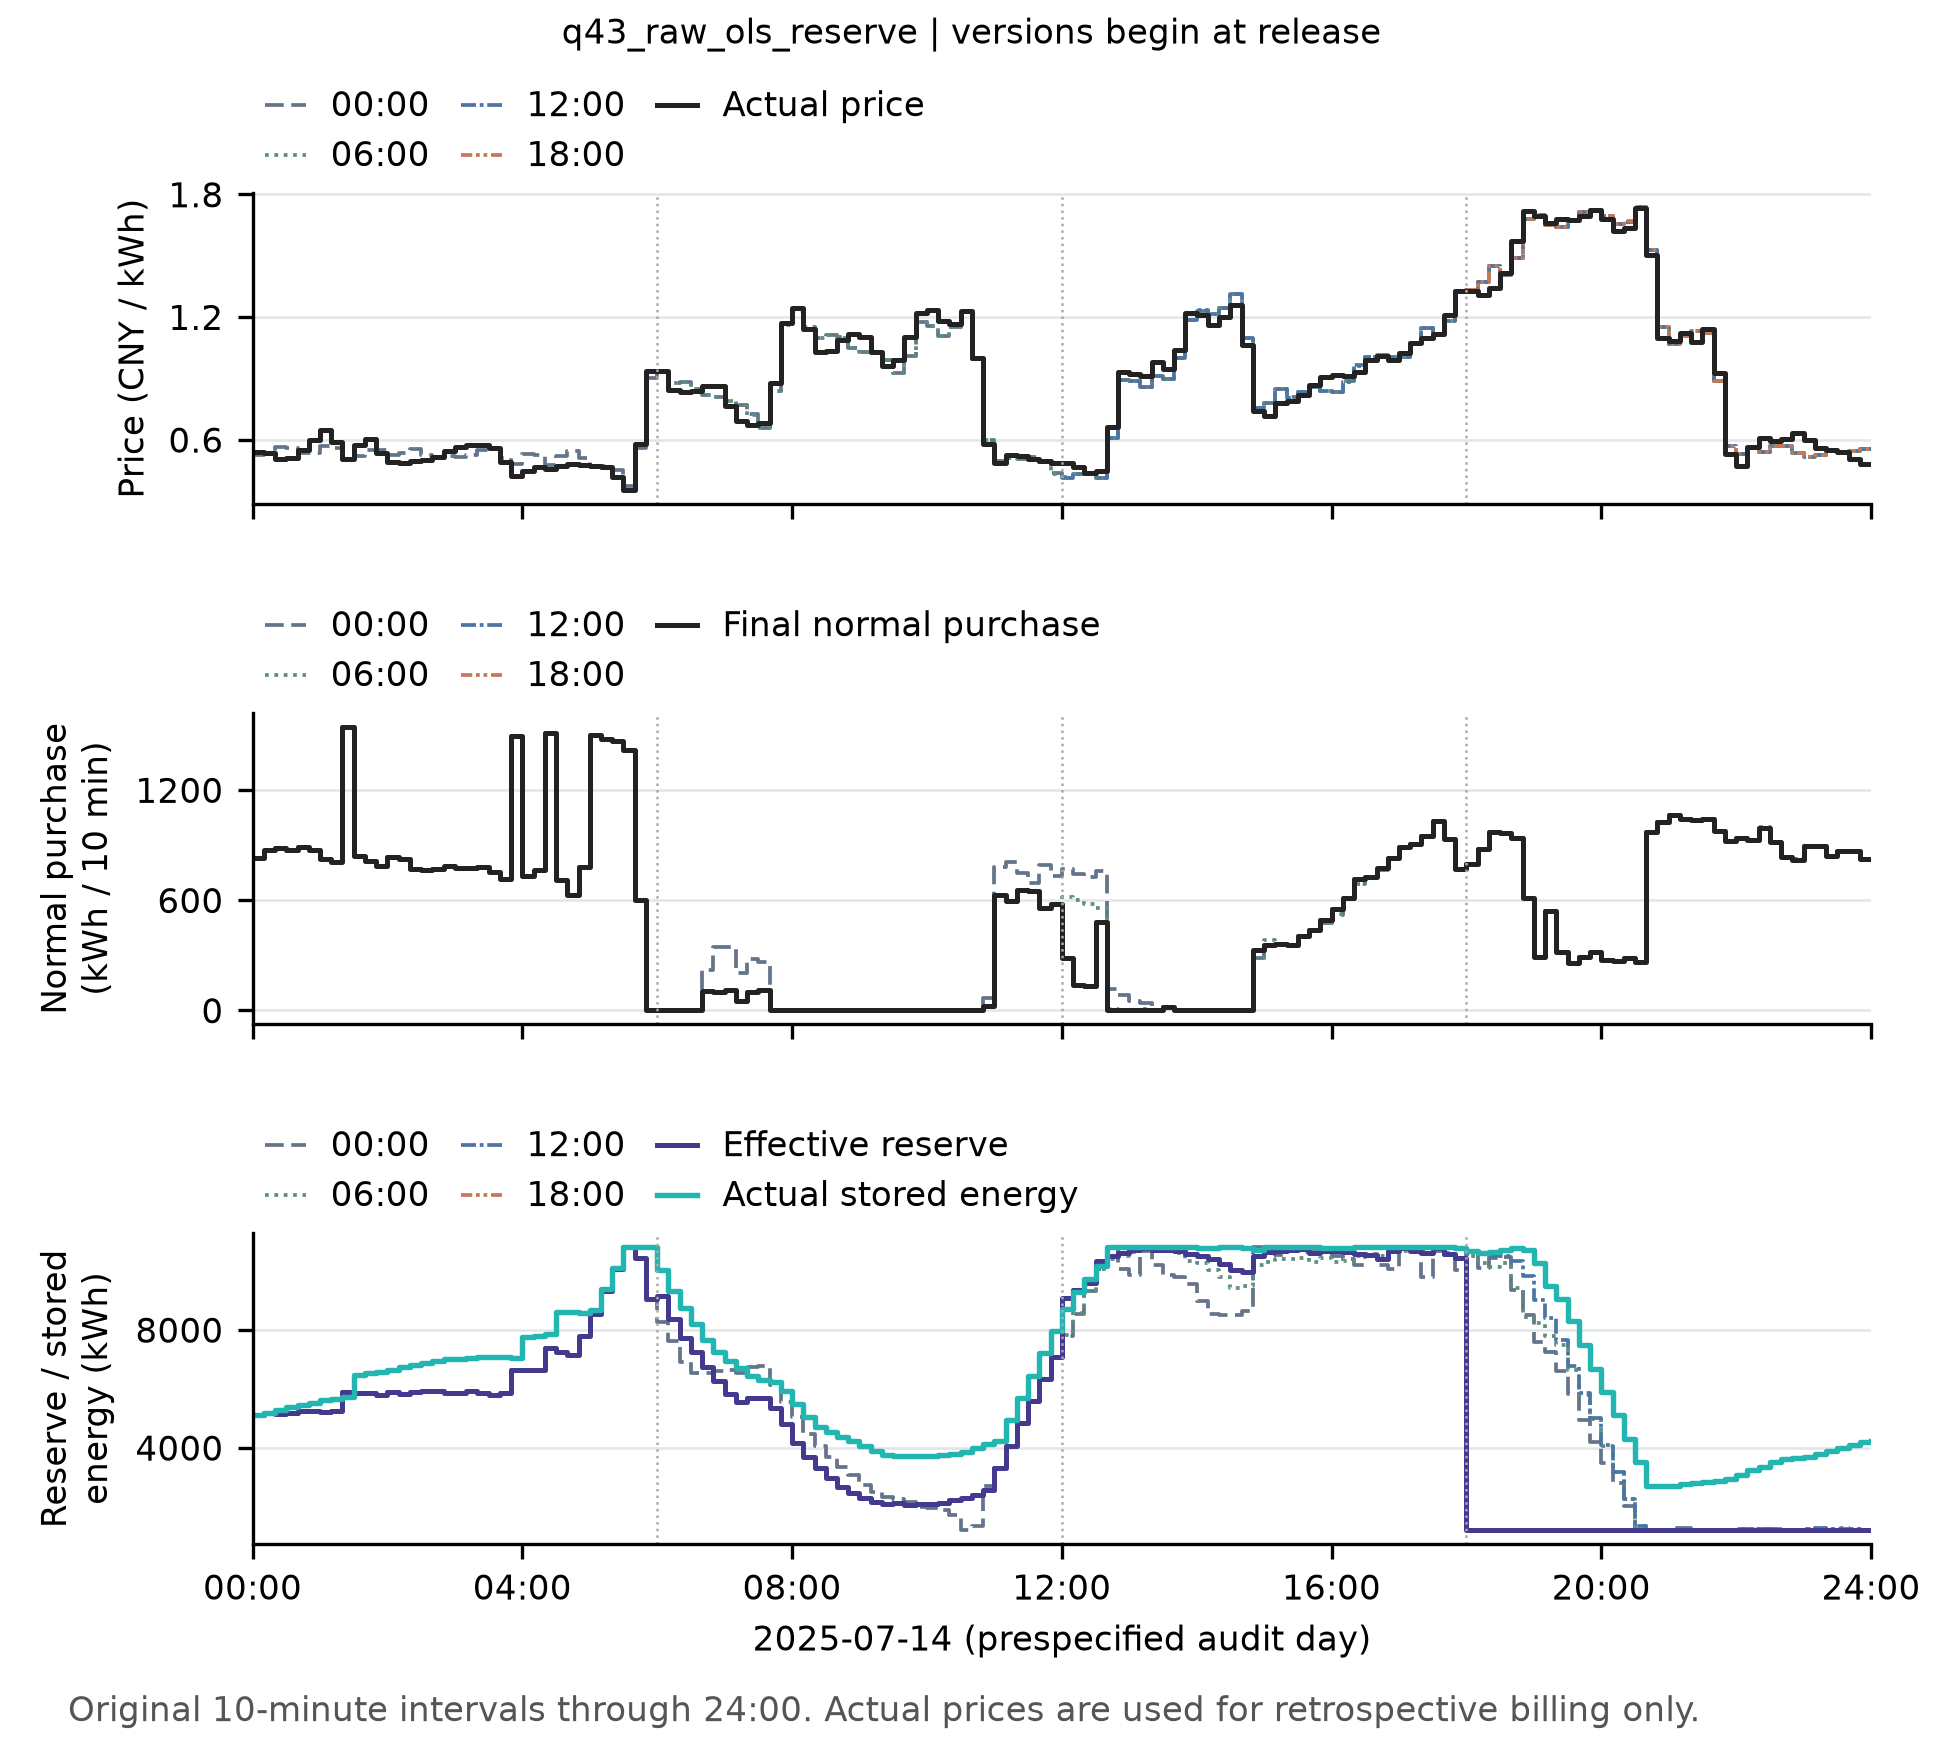
\includegraphics[width=\linewidth,height=150mm,keepaspectratio]{build/figure-08.png}
\caption{Selected Q4-3 policy on 14 July 2025: released planning prices, purchase versions, and storage energy with executed reserve thresholds. Future versions begin only at 00:00, 06:00, 12:00, or 18:00. Actual prices are retrospective settlement data, and final normal purchases exclude emergencies.}
\label{fig:8}
\end{figure}

Both Q4 branches carry their own actual state continuously. Q4-2 has midnight historical-PV decisions; Q4-3 has released PV, paid revisions, and state feedback. Their absolute bill difference therefore combines several changes and is not a pure estimate of PV information value. No new Q4 no-update or state-only controls were added. The supported price comparisons are the within-controller, within-PV pairs in Table 15.

The four selected reserve policies are also compared with their frozen v5 predecessors in Section 8. Those references retain their original two-search budget and historical selection, so they show the effect of replacing the previous selections. The four-search greedy arm provides the more closely matched controller comparison.

\section{Correctness, sensitivity, and historical uncertainty}\label{correctness-sensitivity-and-historical-uncertainty}

\subsection{Implementation, information cutoffs, and reproduction}\label{implementation-information-cutoffs-and-reproduction}

\begingroup
\interlinepenalty=10000
\brokenpenalty=10000

Independent verification rebuilt the source inputs and refitted historical forecasts at their own information cutoffs, using implementations separate from the production forecast, execution, billing, and objective functions. It replayed all twenty-two annual paths and checked candidate scores and saved workbooks. Table 9 reports the numerical discrepancies and tolerances; Appendix A records the coverage and reproduction details.

\par
\endgroup

% TABLE-BEGIN 9
\Needspace{169.9pt}
\begingroup
\fontsize{9.0}{10.8}\selectfont
\setlength{\tabcolsep}{3.2pt}
\renewcommand{\arraystretch}{1.12}
\setlength{\LTleft}{0pt plus 1fill}\setlength{\LTright}{0pt plus 1fill}
\setlength{\LTcapwidth}{\linewidth}

\begin{longtable}[]{@{}
  >{\raggedright\arraybackslash}p{(\linewidth - 6\tabcolsep) * \real{0.2123}}
  >{\raggedright\arraybackslash}p{(\linewidth - 6\tabcolsep) * \real{0.4627}}
  >{\raggedright\arraybackslash}p{(\linewidth - 6\tabcolsep) * \real{0.2000}}
  >{\raggedright\arraybackslash}p{(\linewidth - 6\tabcolsep) * \real{0.1249}}@{}}
\caption{Recorded v6 verification evidence and tolerances.}\tabularnewline
\toprule\noalign{}
\begin{minipage}[b]{\linewidth}\raggedright
\textbf{Object}
\end{minipage} & \begin{minipage}[b]{\linewidth}\raggedright
\textbf{Scope of comparison}
\end{minipage} & \begin{minipage}[b]{\linewidth}\raggedright
\textbf{Maximum absolute discrepancy}
\end{minipage} & \begin{minipage}[b]{\linewidth}\raggedright
\textbf{Threshold}
\end{minipage} \\
\midrule\noalign{}
\endfirsthead
\caption[]{Recorded v6 verification evidence and tolerances. (continued)}\tabularnewline
\toprule\noalign{}
\begin{minipage}[b]{\linewidth}\raggedright
\textbf{Object}
\end{minipage} & \begin{minipage}[b]{\linewidth}\raggedright
\textbf{Scope of comparison}
\end{minipage} & \begin{minipage}[b]{\linewidth}\raggedright
\textbf{Maximum absolute discrepancy}
\end{minipage} & \begin{minipage}[b]{\linewidth}\raggedright
\textbf{Threshold}
\end{minipage} \\
\midrule\noalign{}
\endhead
\bottomrule\noalign{}
\endfoot
\bottomrule\noalign{}
\endlastfoot
Physical and forecast energy & Raw source conversion, continuous execution, nominal initializer, and candidate storage paths & \(2.4920\times10^{-9}\) kWh & \(10^{-6}\) kWh \\*
Cash and candidate scores & Full contract, fivefold emergencies, and scenario scores & \(1.8626\times10^{-9}\) CNY & \(10^{-5}\) CNY \\*
Saved workbooks: energy & All five actual XLSX files, specified dates, and physical time keys & \(8.7311\times10^{-11}\) kWh & \(10^{-6}\) kWh \\*
Saved workbooks: fees & Actual saved quantities rebilled from original prices & \(1.1548\times10^{-7}\) CNY & \(10^{-5}\) CNY \\*
Joint derivatives away from kinks & 720 purchase/reserve coordinates at horizons 36, 72, 108, and 144; step 0.001 kWh & \(5.0546\times10^{-8}\) CNY/kWh & \(10^{-5}\) CNY/kWh \\*
\end{longtable}

\endgroup
% TABLE-END 9

The workbook checks read the saved XLSX files directly and reconciled each variable-price emergency event with its independently checked ten-minute ledger allocation. Table 9 reports the energy and fee discrepancies for these saved quantities.

The motivating two-interval test fixes zero normal purchases, two 100 kWh deficits, initial energy 1,311.111111 kWh, and tariffs 0.4248/1.162 CNY/kWh. Greedy discharge costs CNY 581 in emergencies; retaining the battery for the second deficit costs CNY 212.4, with both paths ending at 1,200 kWh. The code reproduces that admissible counterexample. This refutes compulsory-discharge optimality, but the CNY 368.6 difference is not an estimate of annual loss. Boundary cases, scalar/vector recursion comparisons, finite differences away from kinks, and a separate core review check the new mechanism. At a kink the implemented branch derivative is not asserted to be a unique classical derivative.

Independent score accumulation gave a different first qualifying index in 2 numerically tied decisions. Each saved choice obeyed the original \(10^{-8}\) CNY first-index rule on its saved scores. Recomputed scores stayed within the cash tolerance, and accepted index differences corresponded to purchase and reserve vectors agreeing within \(10^{-6}\) kWh. The verification record lists the score gaps.

Twenty-nine information tests used six preselected decision fixtures on 15 May: eighteen interventions on unavailable information, nine positive controls using permitted inputs, and two PV-access guards. Changing future demand/PV, unreleased PV forecasts, or future actual prices left the available inputs, full purchase/reserve candidates, scores, and selected pairs unchanged. Permitted PV, completed price history, and actual-energy changes produced the expected responses. The tests disabled price caches and kept the B0 archive fixed; its historical reconstruction was checked separately. The Q4-2 guard enforced the working interpretation in Table 3.

An isolated reproduction of the selected reserve policies rebuilt the kernel and reproduced the saved trajectories and candidate/input arrays exactly. It used the same host and dependency versions; Appendix A specifies the comparisons and exclusions.

Of 85,504 local searches across twenty-two annual policies, 46,365 ended with non-success stopping records. The logs contain 0 solver exceptions, 0 initializer fallbacks, and 0 invalid-return fallbacks. Selection retained a starting candidate 12 times and the complete keep-current pair 3,047 times. Every finite retained pair was rescored before selection and executed through the hard physical rule. Independent rebilling of the saved ledgers, using separately validated prices, also recomputed all twenty-two summaries and twenty-nine named paired comparisons.

\begingroup
\interlinepenalty=10000
\brokenpenalty=10000

Figure 9 compares midnight forecasts with the latest release permitted by the 00:00/06:00/12:00/18:00 protocol on the selected raw-PV/OLS Q4-3 reserve path. The PV panels share 26,880 intervals with positive actual generation. This subset is chosen retrospectively for evaluation and excludes 21,216 zero-generation intervals, including 1,280 positive forecasts in each version. It leaves forecast-time inputs unchanged. PV MAE falls from 60.77 to 31.83 kWh per ten-minute interval on the subset and from 34.44 to 18.27 kWh over all 48,096 intervals. Price MAE changes from 0.04270 to 0.04240 CNY/kWh. These error summaries cover one retained historical path; Table 15 gives the matched policy comparisons used to assess operating costs.

\par
\endgroup

\begin{figure}[!htbp]
\centering
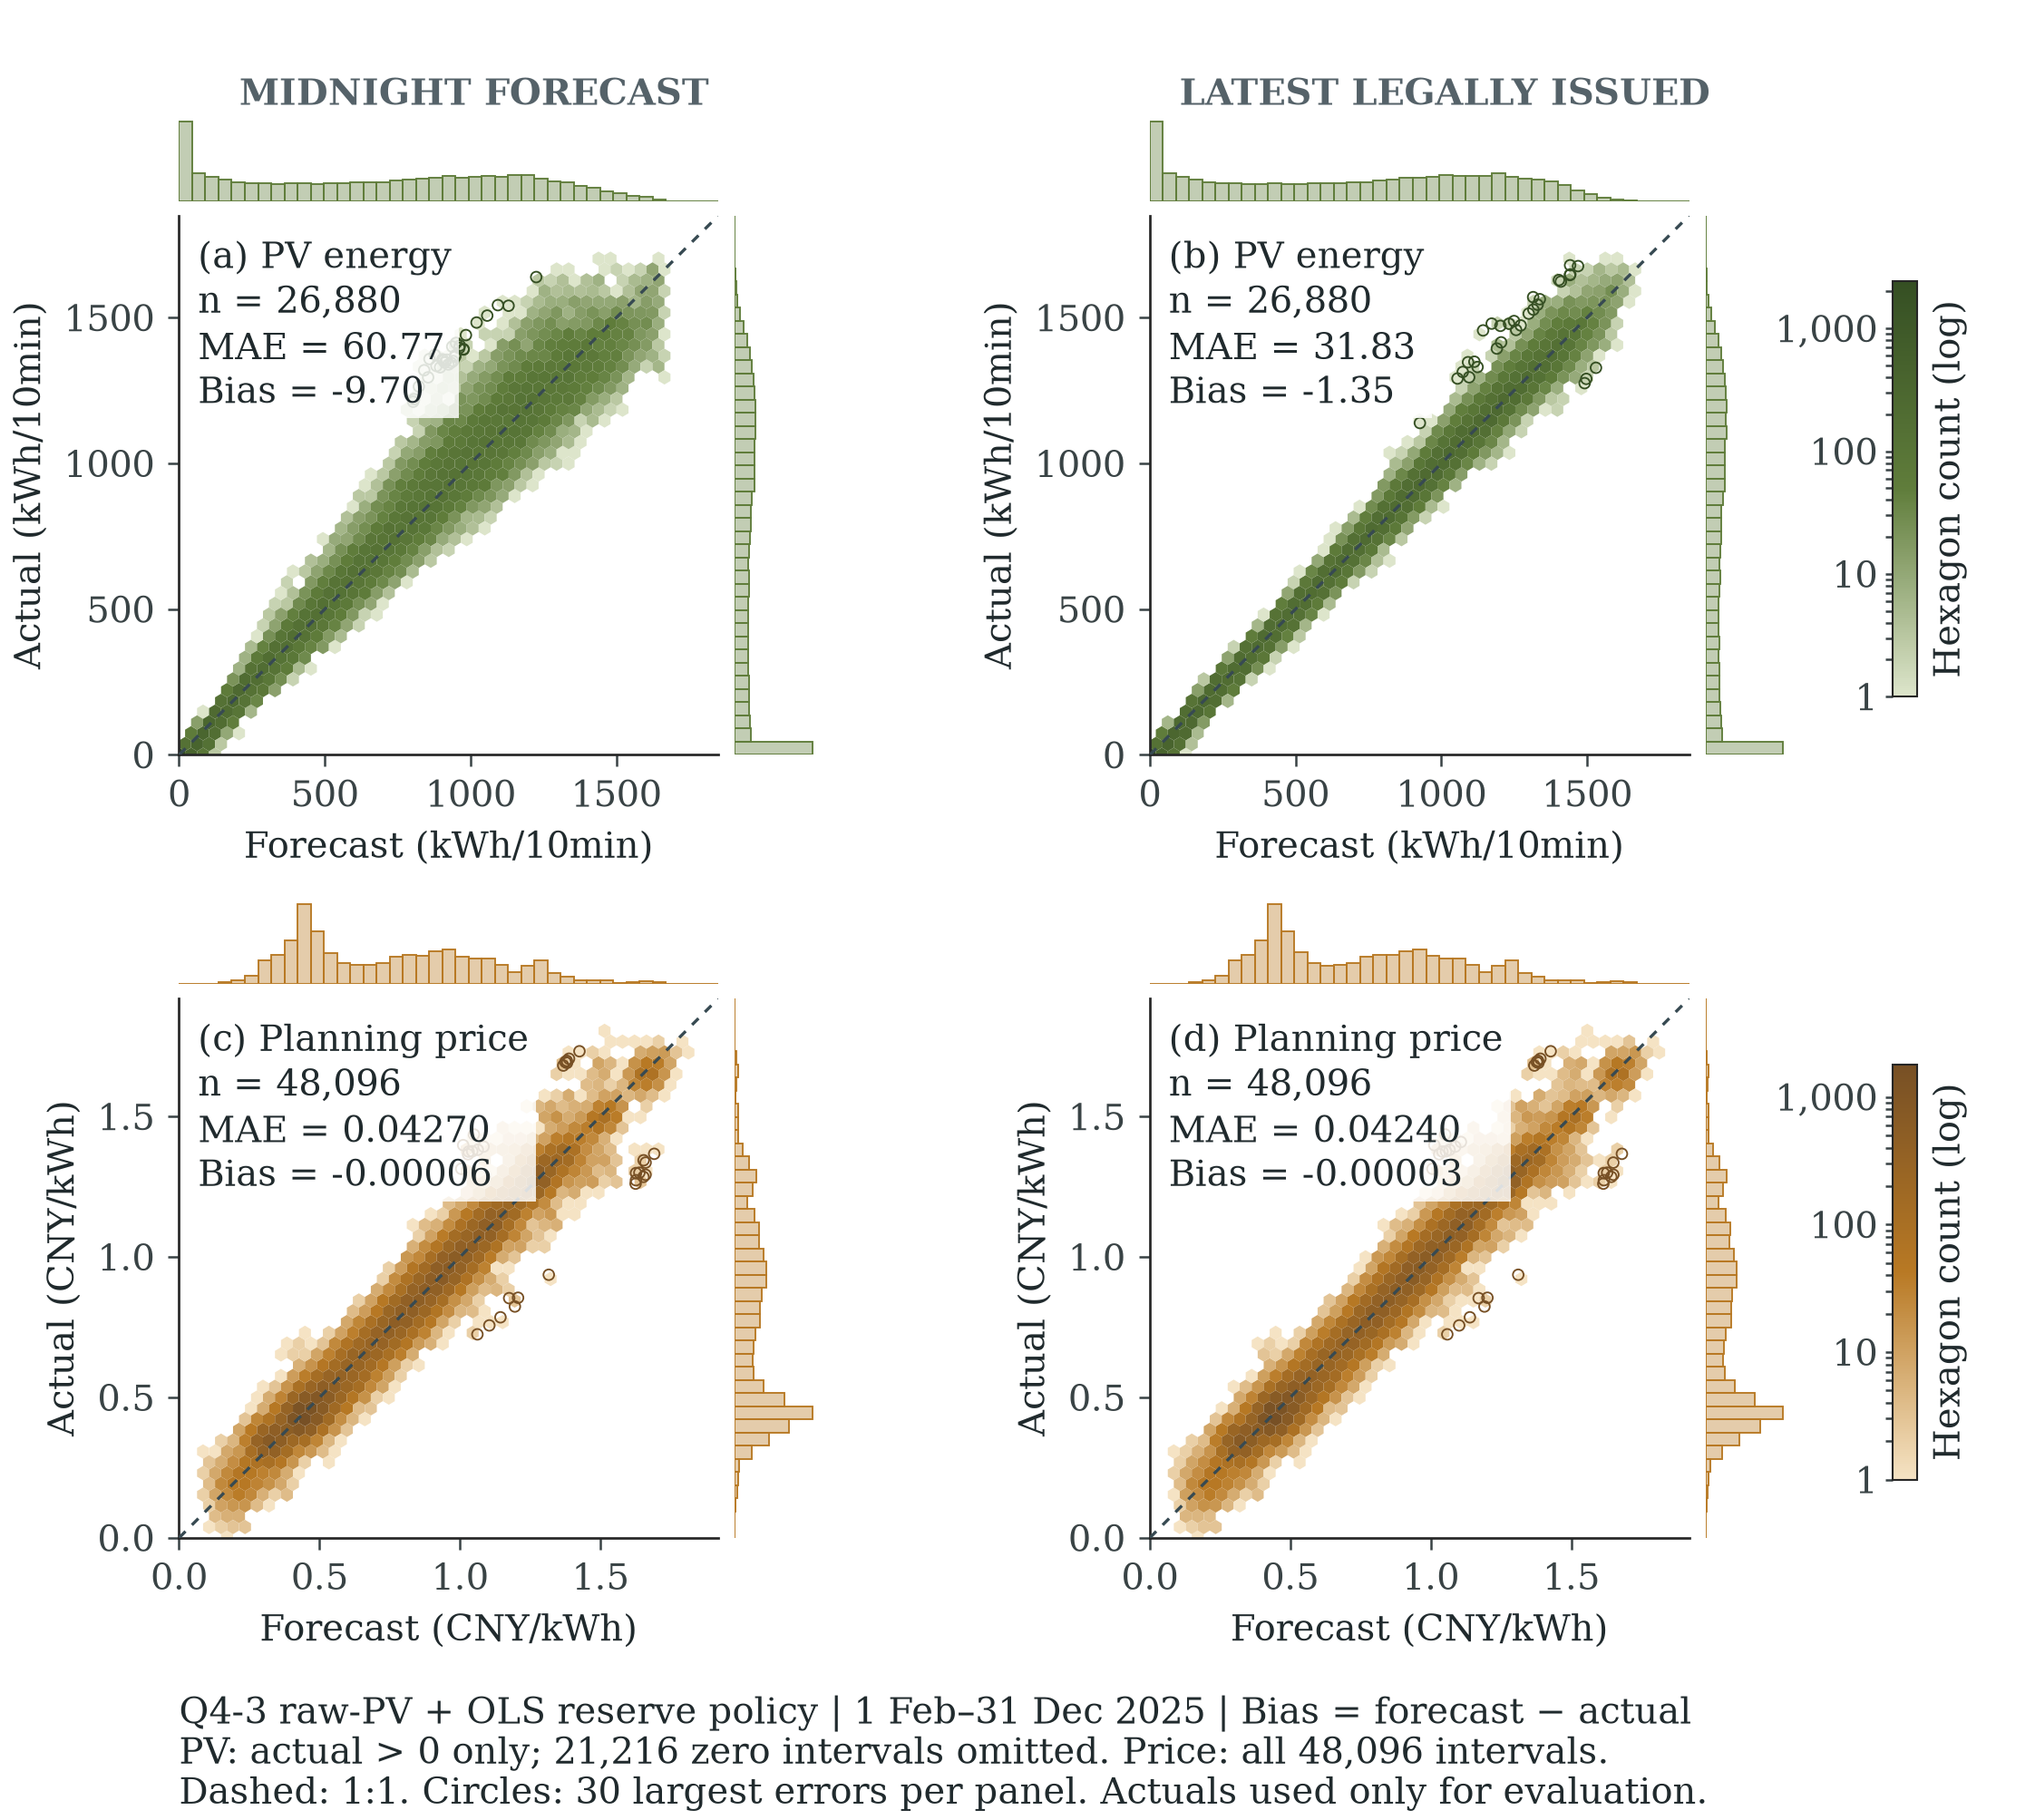
\includegraphics[width=\linewidth,height=150mm,keepaspectratio]{build/figure-09.png}
\caption{Forecast-actual distributions for the selected raw-PV/OLS Q4-3 reserve policy, February-December 2025. PV panels use the same actual-positive subset (26,880 intervals); price panels use all 48,096 intervals. Forecast versions are aligned by date, interval, and permitted issue time. Hexagons show counts on a shared logarithmic scale within each row; marginals show counts, dashed lines show equality, and circles mark the 30 largest absolute errors per panel. Bias is forecast minus actual. Actual values are retrospective evaluation outcomes.}
\label{fig:9}
\end{figure}

\subsection{Paired savings, losing periods, and terminal inventory}\label{paired-savings-losing-periods-and-terminal-inventory}

\begingroup
\interlinepenalty=10000
\brokenpenalty=10000

For candidate \(a\) and reference \(b\), daily saving is \(S_d=B_d^b-B_d^a\). Positive values favor the candidate; monthly and annual savings sum these same matched daily differences. The denominator of a saving percentage is the named reference\textquotesingle s total cash bill. Each selected reserve policy is paired below with the same input configuration in the four-search greedy arm.

\par
\endgroup

\begingroup
\interlinepenalty=10000
\brokenpenalty=10000

Figure 10 shows why winning on many days need not reduce the annual bill: the selected Q3 reserve policy saves money on 188 of 334 days but costs CNY 6,206.07 more over the full period. The plotted observations retain both tails; Table 10 gives the annual block intervals.

\par
\endgroup

\begin{figure}[!htbp]
\centering
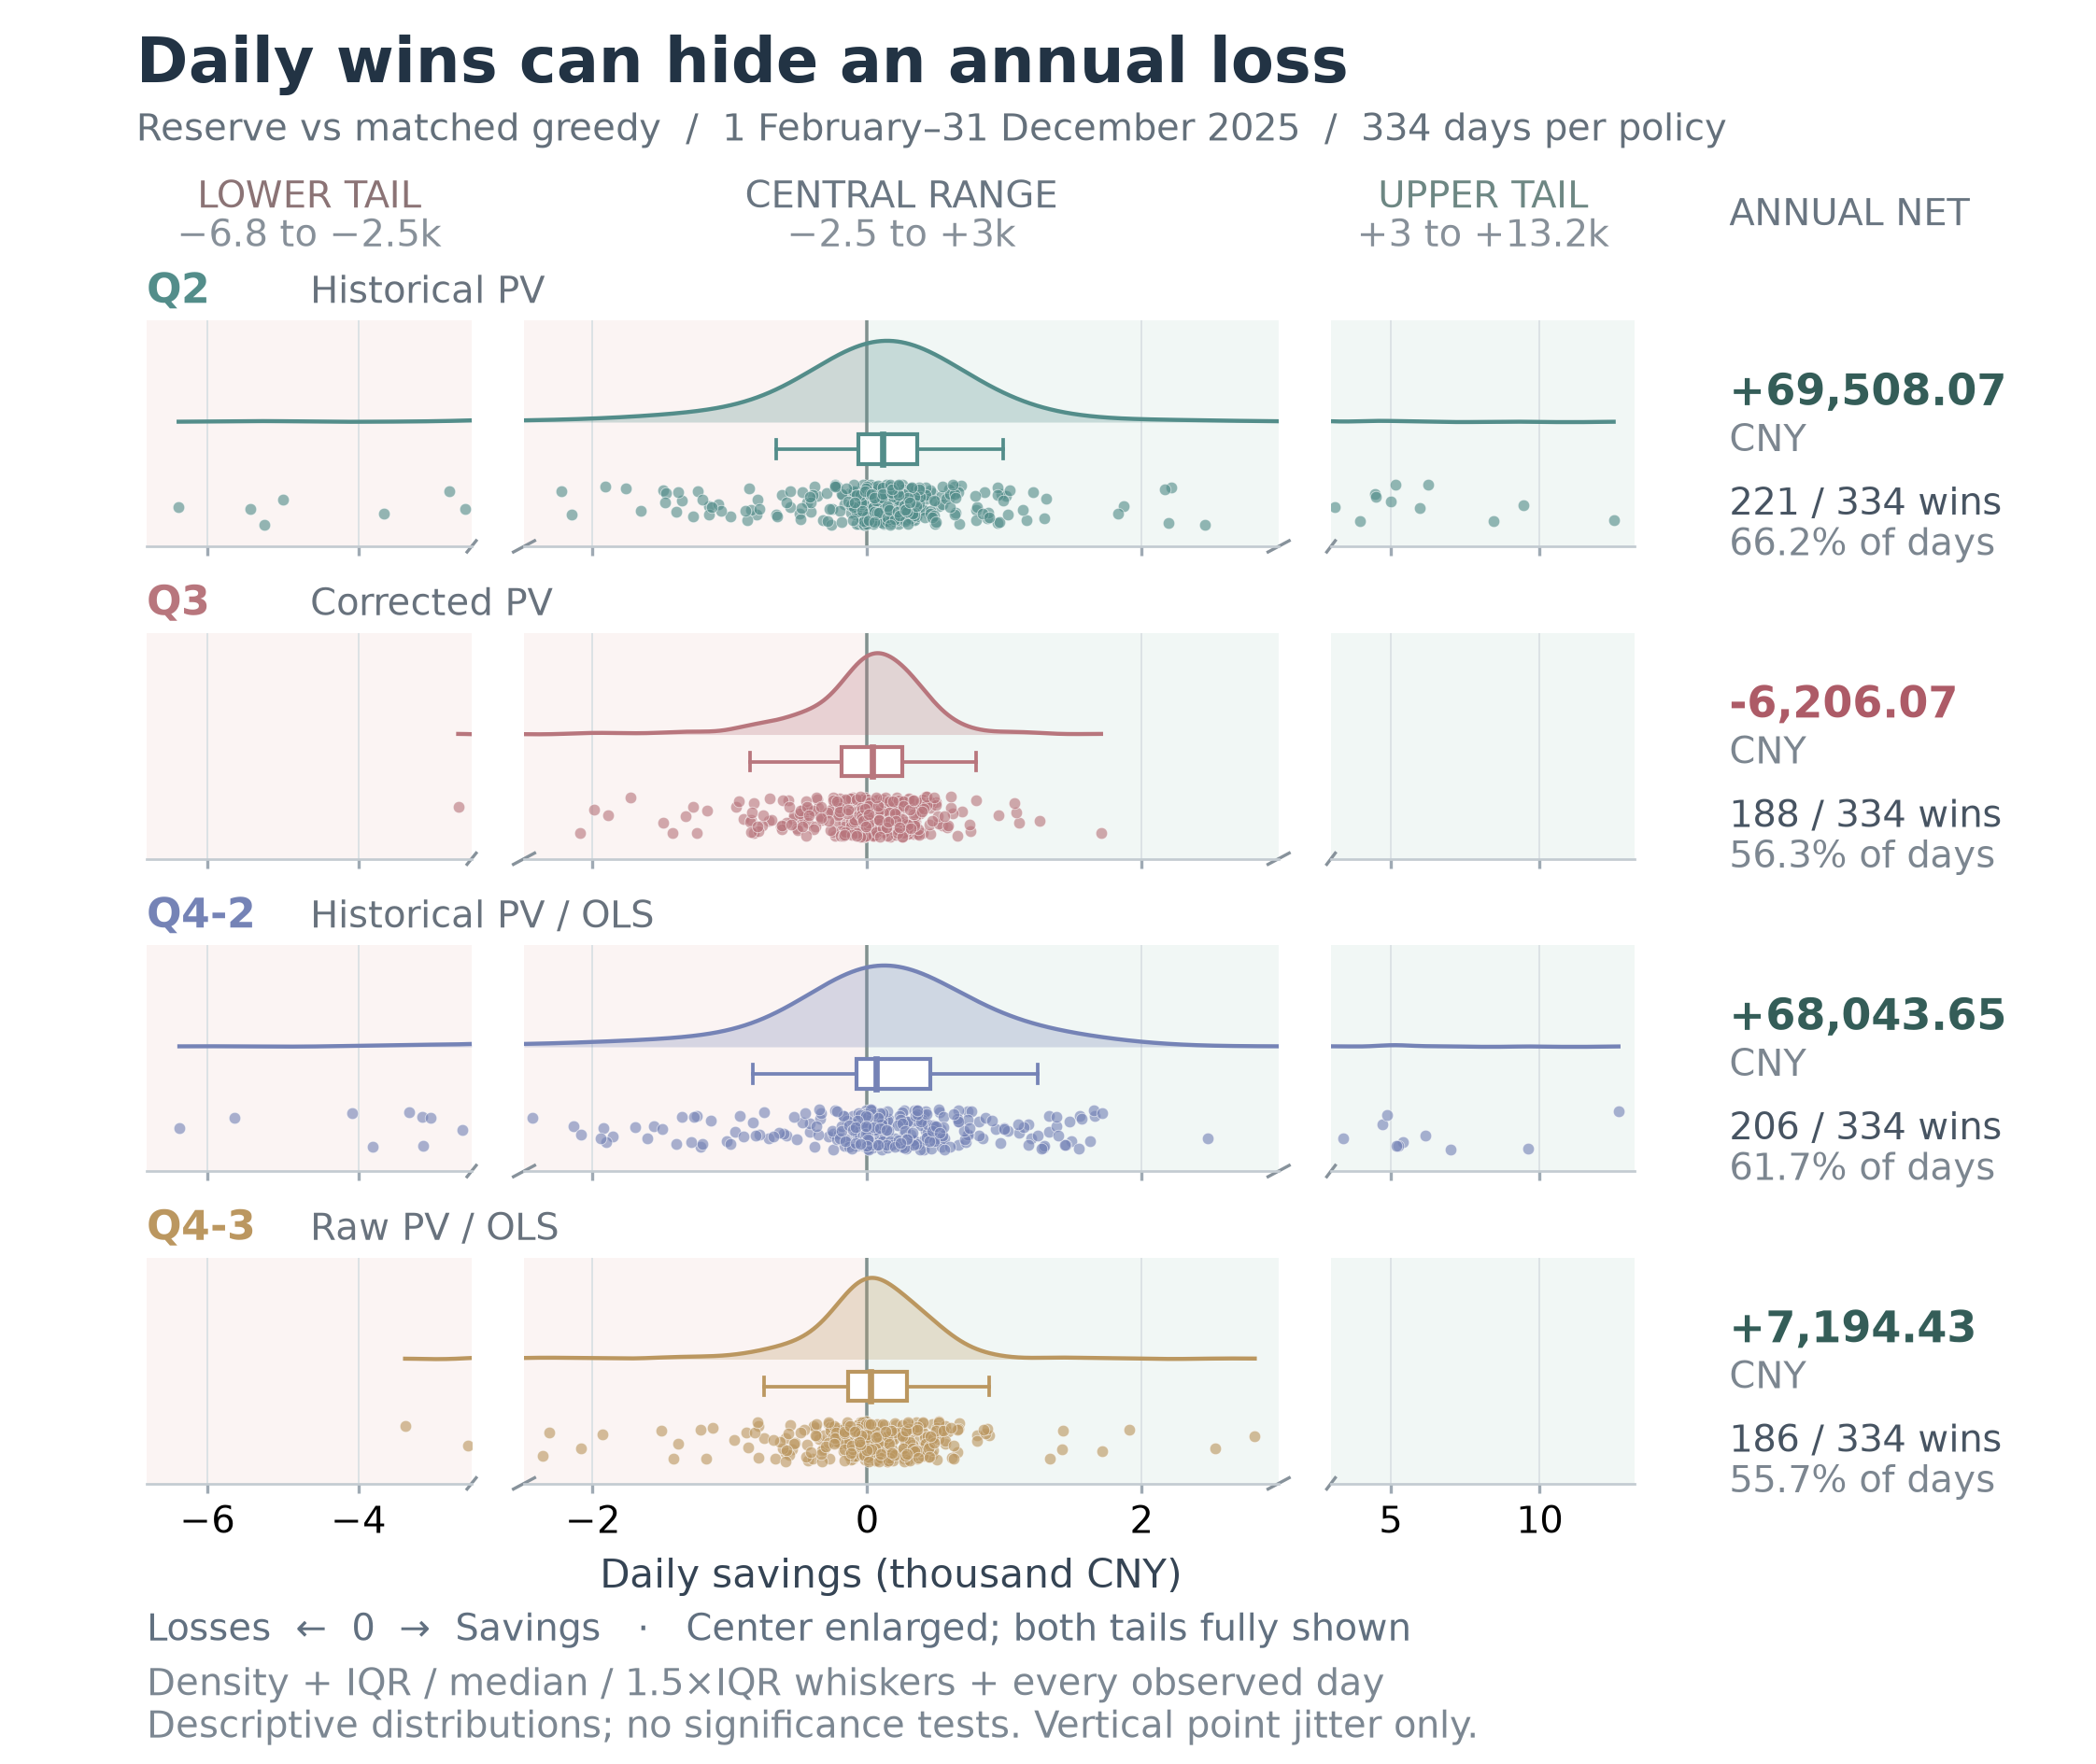
\includegraphics[width=\linewidth,height=150mm,keepaspectratio]{build/figure-10.png}
\caption{Daily cash savings relative to each selected policy\textquotesingle s same-configuration four-search greedy control, February-December 2025. Each row contains all 334 days. Positive values favor reserve. Three adjoining horizontal ranges retain both tails while enlarging the center; their scales differ. Half-violins use Scott-bandwidth density estimates normalized to each row\textquotesingle s peak and show shape only; plotted areas and heights are not probability comparisons. Boxes show the median and interquartile range, with 1.5-IQR whiskers; dots are original daily values with vertical jitter. Annual net savings and winning-day counts use the full rows.}
\label{fig:10}
\end{figure}

% TABLE-BEGIN 10
\Needspace{101.5pt}
\begingroup
\fontsize{8.6}{10.32}\selectfont
\setlength{\tabcolsep}{3.2pt}
\renewcommand{\arraystretch}{1.12}
\setlength{\LTleft}{0pt plus 1fill}\setlength{\LTright}{0pt plus 1fill}
\setlength{\LTcapwidth}{\linewidth}

\begin{longtable}[]{@{}
  >{\raggedright\arraybackslash}p{(\linewidth - 8\tabcolsep) * \real{0.0859}}
  >{\raggedright\arraybackslash}p{(\linewidth - 8\tabcolsep) * \real{0.2010}}
  >{\raggedleft\arraybackslash}p{(\linewidth - 8\tabcolsep) * \real{0.1473}}
  >{\raggedright\arraybackslash}p{(\linewidth - 8\tabcolsep) * \real{0.2818}}
  >{\raggedright\arraybackslash}p{(\linewidth - 8\tabcolsep) * \real{0.2840}}@{}}
\caption{Selected reserve policies versus same-configuration greedy controls, 334 days; CNY. Descriptive 95\% intervals use 2,000 circular-block resamples.}\tabularnewline
\toprule\noalign{}
\begin{minipage}[b]{\linewidth}\raggedright
\textbf{Branch}
\end{minipage} & \begin{minipage}[b]{\linewidth}\raggedright
\textbf{Matched greedy reference}
\end{minipage} & \begin{minipage}[b]{\linewidth}\raggedleft
\textbf{Cash saving}
\end{minipage} & \begin{minipage}[b]{\linewidth}\raggedright
\textbf{7-day interval}
\end{minipage} & \begin{minipage}[b]{\linewidth}\raggedright
\textbf{14-day interval}
\end{minipage} \\
\midrule\noalign{}
\endfirsthead
\caption[]{Selected reserve policies versus same-configuration greedy controls, 334 days; CNY. Descriptive 95\% intervals use 2,000 circular-block resamples. (continued)}\tabularnewline
\toprule\noalign{}
\begin{minipage}[b]{\linewidth}\raggedright
\textbf{Branch}
\end{minipage} & \begin{minipage}[b]{\linewidth}\raggedright
\textbf{Matched greedy reference}
\end{minipage} & \begin{minipage}[b]{\linewidth}\raggedleft
\textbf{Cash saving}
\end{minipage} & \begin{minipage}[b]{\linewidth}\raggedright
\textbf{7-day interval}
\end{minipage} & \begin{minipage}[b]{\linewidth}\raggedright
\textbf{14-day interval}
\end{minipage} \\
\midrule\noalign{}
\endhead
\bottomrule\noalign{}
\endfoot
\bottomrule\noalign{}
\endlastfoot
Q2 & q2\_greedy & 69,508.07 & {[}4,484.52, 160,892.55{]} & {[}3,279.77, 162,427.06{]} \\*
Q3 & q3\_w28\_greedy & -6,206.07 & {[}-26,367.00, 14,137.80{]} & {[}-29,281.12, 16,720.13{]} \\*
Q4-2 & q42\_ols\_greedy & 68,043.65 & {[}1,453.28, 155,787.03{]} & {[}-3,135.99, 158,176.86{]} \\*
Q4-3 & q43\_raw\_ols\_greedy & 7,194.43 & {[}-14,347.68, 30,167.31{]} & {[}-18,423.91, 33,626.59{]} \\*
\end{longtable}

\endgroup
% TABLE-END 10

Both Q2 block intervals are positive. Q4-2\textquotesingle s 14-day interval crosses zero, and both intervals cross zero for Q3 and Q4-3. Every selected reserve policy has losing months against its matched greedy control; favorable annual totals do not imply uniform benefit.

\begingroup
\interlinepenalty=10000
\brokenpenalty=10000

Figure 11 extends the monthly comparison to all eleven matched configurations. Color is the monthly cash saving as a percentage of that configuration\textquotesingle s greedy bill, so it is not an absolute-cost ranking. Rows are ordered by average-linkage Euclidean clustering of their standardized monthly percentage profiles; the displayed colors remain unstandardized and months remain chronological. The side tracks show annual cash saving and additional emergency energy, making the cost and emergency-use tradeoff visible. These are comparisons of the complete procurement-and-storage procedures, not isolated effects of changing a reserve threshold while holding procurement fixed.

\par
\endgroup

\begin{figure}[!tp]
\centering
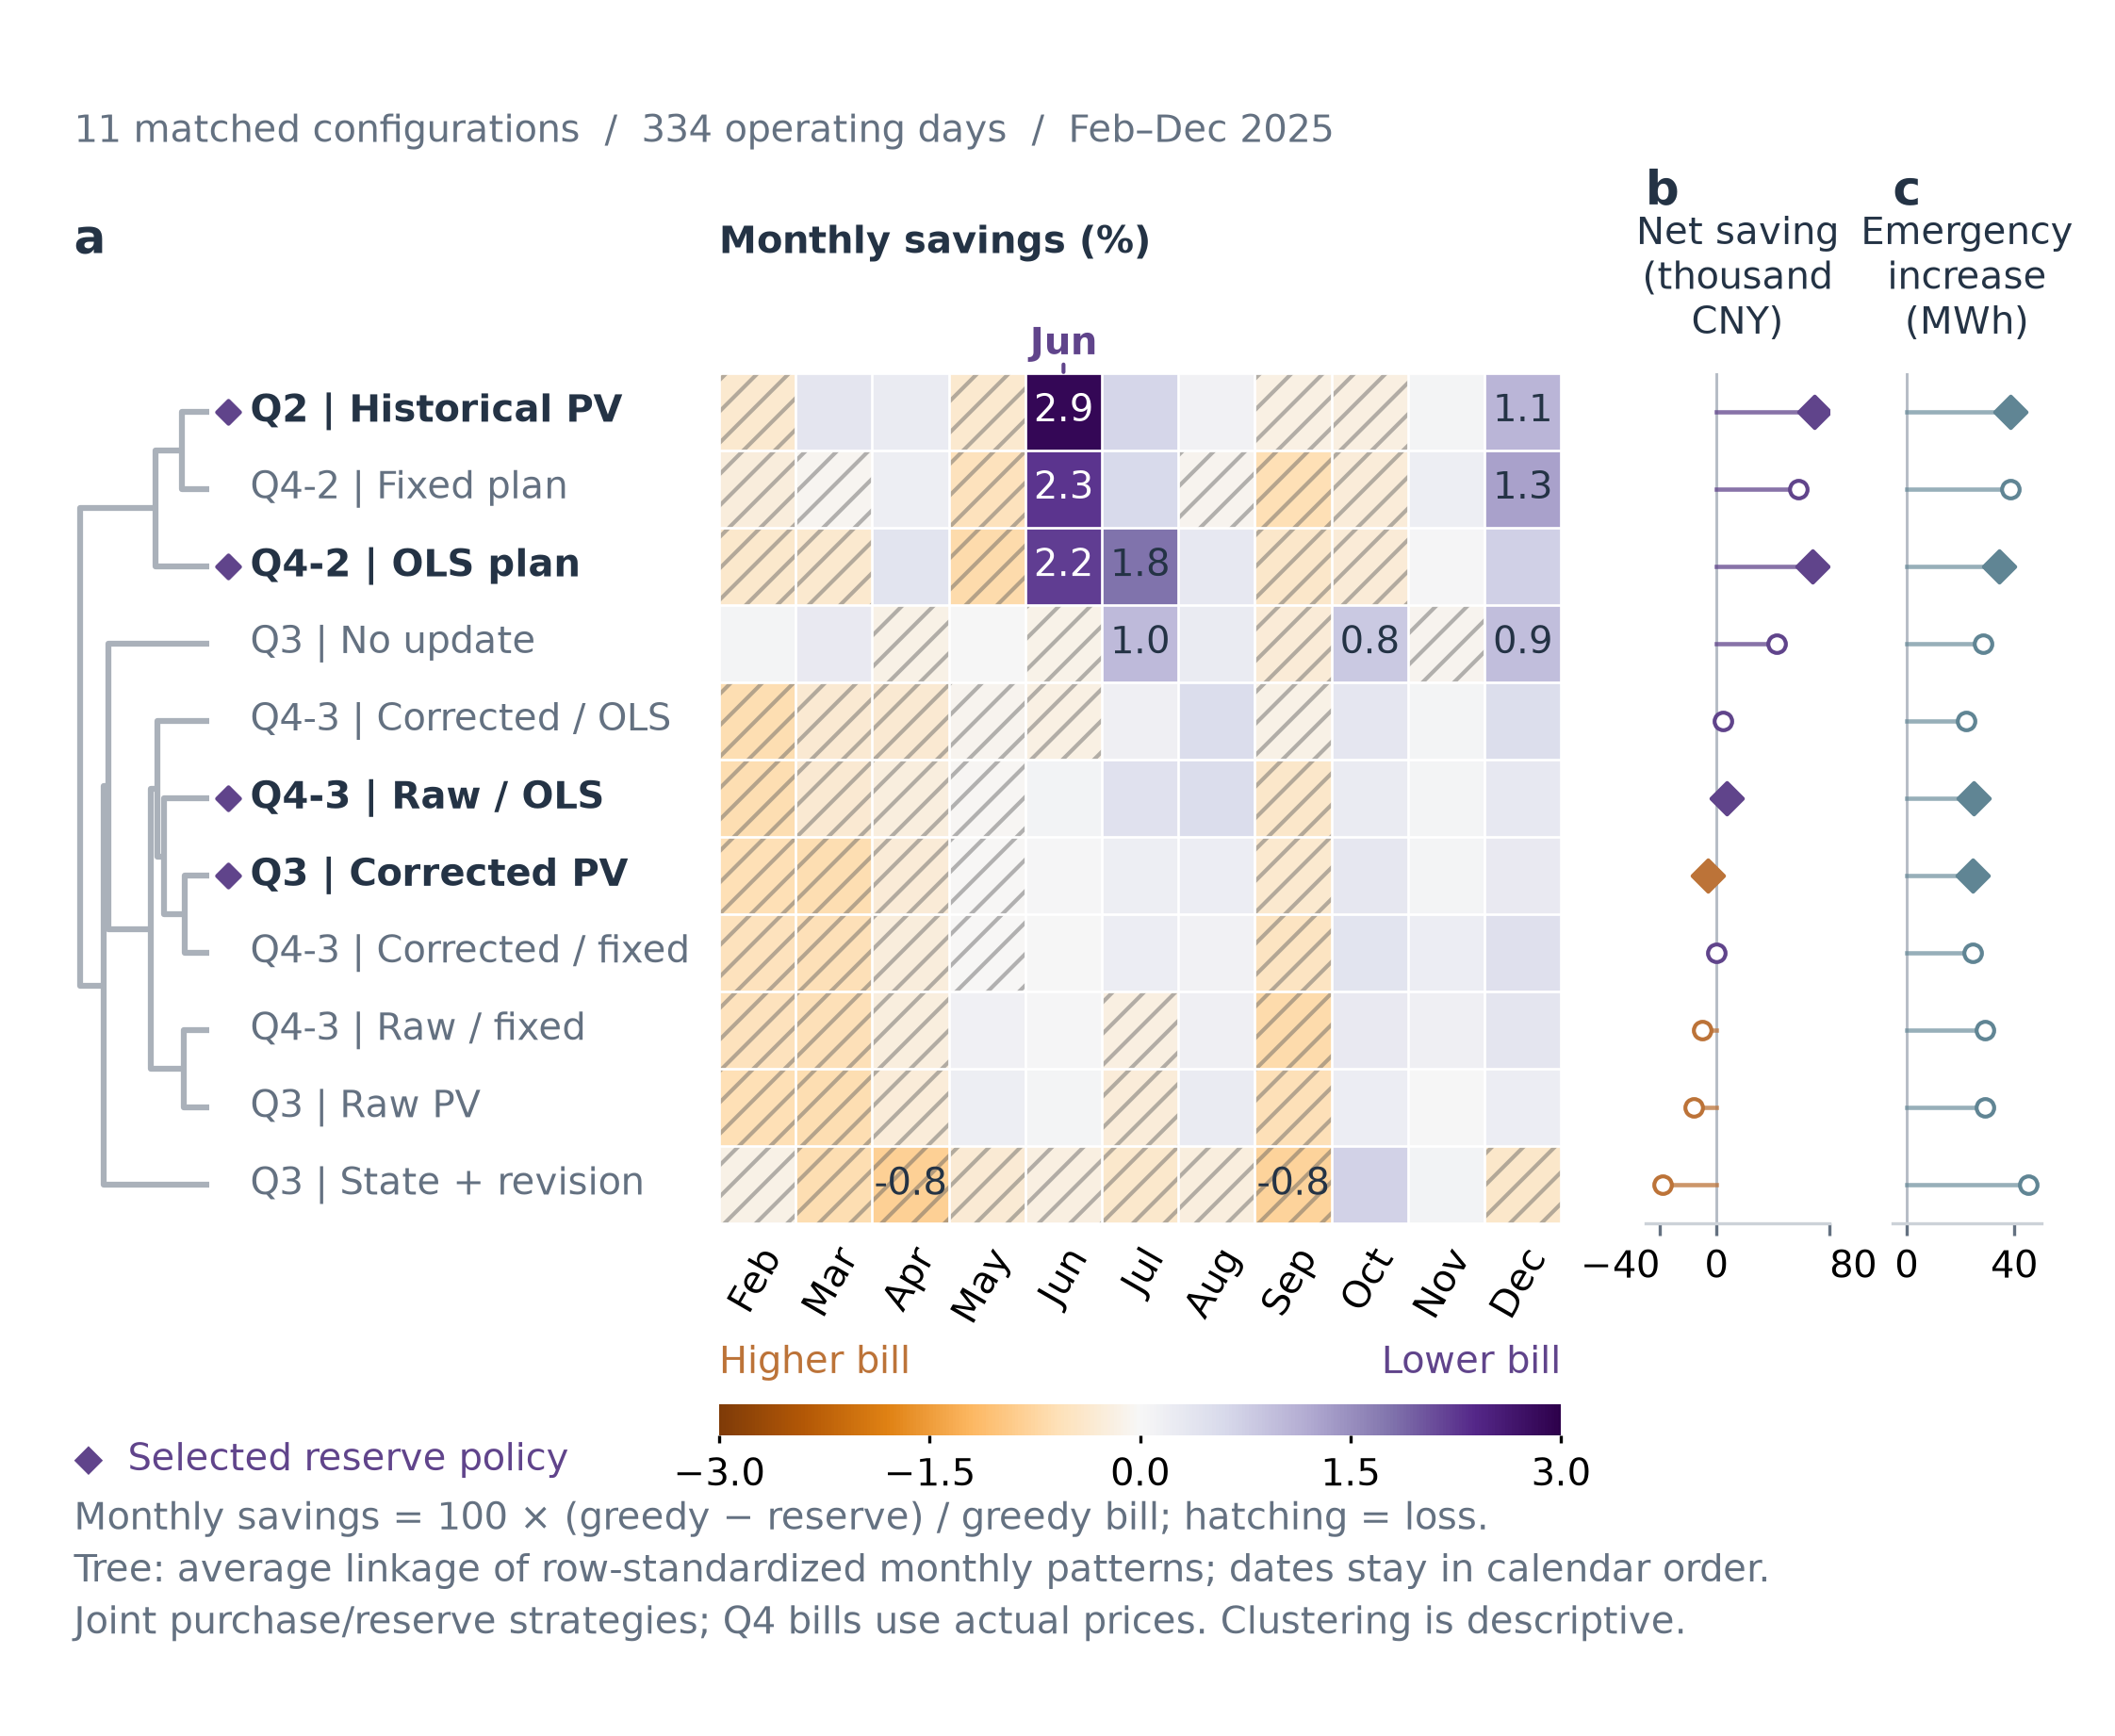
\includegraphics[width=\linewidth,height=150mm,keepaspectratio]{build/figure-11.png}
\caption{Seasonal savings profiles across all eleven reserve/greedy pairs, February-December 2025. Heatmap values are 100 times the monthly greedy-minus-reserve cash difference divided by the matched greedy monthly bill. Standardization affects the descriptive tree and row order only. Side tracks show annual net saving (thousand CNY) and reserve-minus-greedy emergency energy (MWh); diamonds mark the four selected reserve policies. Q4 fixed/OLS labels identify planning prices, while bills use actual prices. Hatching marks negative monthly savings.}
\label{fig:11}
\end{figure}

\Needspace{5\baselineskip}

Table 11 uses the same four pairs to show endpoint energy and an auxiliary inventory adjustment:

\[
S_{\mathrm{inventory}}=\sum_d S_d+
\nu(E_{\mathrm{end}}^a-E_{\mathrm{end}}^b). \tag{11}
\]

The diagnostic rate is \(\nu=\eta_d\overline p=0.9\times0.7661972222\ldots=0.6895775\) CNY/kWh, where \(\overline p\) is the arithmetic mean of the 144 Attachment 1 tariff entries. It values one internal kWh by its discharge efficiency at the mean fixed tariff and was inherited as a common endpoint diagnostic. It is separate from the planning coefficient \(\mu=0.38232\), is not fitted to the selected v6 cost savings, and is neither a sale tariff nor cash income. An endpoint adjustment does not reoptimize trajectories or remove losses earlier in the year.

% TABLE-BEGIN 11
\Needspace{91.3pt}
\begingroup
\fontsize{8.6}{10.32}\selectfont
\setlength{\tabcolsep}{3.2pt}
\renewcommand{\arraystretch}{1.12}
\setlength{\LTleft}{0pt plus 1fill}\setlength{\LTright}{0pt plus 1fill}
\setlength{\LTcapwidth}{\linewidth}

\begin{longtable}[]{@{}
  >{\raggedright\arraybackslash}p{(\linewidth - 8\tabcolsep) * \real{0.1180}}
  >{\raggedleft\arraybackslash}p{(\linewidth - 8\tabcolsep) * \real{0.2386}}
  >{\raggedleft\arraybackslash}p{(\linewidth - 8\tabcolsep) * \real{0.2386}}
  >{\raggedleft\arraybackslash}p{(\linewidth - 8\tabcolsep) * \real{0.2024}}
  >{\raggedleft\arraybackslash}p{(\linewidth - 8\tabcolsep) * \real{0.2024}}@{}}
\caption{Terminal-inventory audit for the same matched comparisons; energy in kWh and savings in CNY.}\tabularnewline
\toprule\noalign{}
\begin{minipage}[b]{\linewidth}\raggedright
\textbf{Branch}
\end{minipage} & \begin{minipage}[b]{\linewidth}\raggedleft
\textbf{Reserve final E}
\end{minipage} & \begin{minipage}[b]{\linewidth}\raggedleft
\textbf{Greedy final E}
\end{minipage} & \begin{minipage}[b]{\linewidth}\raggedleft
\textbf{Cash saving}
\end{minipage} & \begin{minipage}[b]{\linewidth}\raggedleft
\textbf{Inventory-adjusted}
\end{minipage} \\
\midrule\noalign{}
\endfirsthead
\caption[]{Terminal-inventory audit for the same matched comparisons; energy in kWh and savings in CNY. (continued)}\tabularnewline
\toprule\noalign{}
\begin{minipage}[b]{\linewidth}\raggedright
\textbf{Branch}
\end{minipage} & \begin{minipage}[b]{\linewidth}\raggedleft
\textbf{Reserve final E}
\end{minipage} & \begin{minipage}[b]{\linewidth}\raggedleft
\textbf{Greedy final E}
\end{minipage} & \begin{minipage}[b]{\linewidth}\raggedleft
\textbf{Cash saving}
\end{minipage} & \begin{minipage}[b]{\linewidth}\raggedleft
\textbf{Inventory-adjusted}
\end{minipage} \\
\midrule\noalign{}
\endhead
\bottomrule\noalign{}
\endfoot
\bottomrule\noalign{}
\endlastfoot
Q2 & 3,179.368744 & 3,146.715222 & 69,508.07 & 69,530.59 \\*
Q3 & 2,438.521203 & 2,353.164464 & -6,206.07 & -6,147.21 \\*
Q4-2 & 2,989.756760 & 3,280.866789 & 68,043.65 & 67,842.90 \\*
Q4-3 & 2,514.150453 & 2,397.432892 & 7,194.43 & 7,274.91 \\*
\end{longtable}

\endgroup
% TABLE-END 11

\begingroup
\interlinepenalty=10000
\brokenpenalty=10000

Against the frozen two-search v5 selections, the new selected reserve policies have signed cash savings of CNY 68,439.49 (Q2), -12,628.36 (Q3), 60,020.48 (Q4-2), and 8,221.27 (Q4-3). Negative saving denotes increased expenditure. These combine controller, search-budget, and any input-selection changes, so they are not substituted for the matched controller comparisons.

\par
\endgroup

\begingroup
\interlinepenalty=10000
\brokenpenalty=10000

Circular block resampling retains neighboring daily differences and wraps at the endpoints {[}9{]}. Both block lengths use 2,000 resamples with seed 20260915. The procedure resamples fixed historical cost differences: it neither reruns the battery on new weather nor refits forecasts, and it leaves repeated 2025 selection uncorrected. Its intervals therefore provide no selection-adjusted inference for unseen years or causal effects. The density displays and descriptive clustering summarize observed variation without significance tests. Scenario ordering was preserved; a shuffled-scenario comparison was not performed.

\par
\endgroup

Q1\textquotesingle s efficiency-by-power-side cases address the supplied physical ambiguity. The earlier Q2 history-window, cost-weight, and optimizer-budget cases concern the original greedy workflow. The current twenty-two-policy matrix fixes those inherited parameters and compares storage control, information permissions, planning prices, and PV correction. Earlier 275-day reserve/update-gate and correction cases remain explicitly historical in Appendix B. None establishes robustness of the new controller to different capacities, degradation, sustained forecast bias, or unseen years.

\section{Evaluation and final operating policies}\label{evaluation-and-final-operating-policies}

The model chooses when to retain battery energy together with normal procurement. The same reserve rule evaluates historical scenarios and executes actual intervals, preserving physical limits and the full fivefold emergency price. Paid procurement updates retain the whole current purchase/reserve pair and freeze executed quantities. Planning prices affect decisions; actual prices determine cash settlement. Together, these rules allow the controller to retain energy for later deficits instead of requiring immediate discharge.

% TABLE-BEGIN 12
\Needspace{107.7pt}
\begingroup
\fontsize{8.3}{9.96}\selectfont
\setlength{\tabcolsep}{3.2pt}
\renewcommand{\arraystretch}{1.12}
\setlength{\LTleft}{0pt plus 1fill}\setlength{\LTright}{0pt plus 1fill}
\setlength{\LTcapwidth}{\linewidth}

\begin{longtable}[]{@{}
  >{\raggedright\arraybackslash}p{(\linewidth - 10\tabcolsep) * \real{0.0785}}
  >{\raggedright\arraybackslash}p{(\linewidth - 10\tabcolsep) * \real{0.3085}}
  >{\raggedright\arraybackslash}p{(\linewidth - 10\tabcolsep) * \real{0.1598}}
  >{\raggedleft\arraybackslash}p{(\linewidth - 10\tabcolsep) * \real{0.1652}}
  >{\raggedleft\arraybackslash}p{(\linewidth - 10\tabcolsep) * \real{0.1345}}
  >{\raggedleft\arraybackslash}p{(\linewidth - 10\tabcolsep) * \real{0.1535}}@{}}
\caption{Five final policies: cash fees in CNY and final stored energy in kWh. Q1 is one day; annual branches cover 334 days.}\tabularnewline
\toprule\noalign{}
\begin{minipage}[b]{\linewidth}\raggedright
\textbf{Branch}
\end{minipage} & \begin{minipage}[b]{\linewidth}\raggedright
\textbf{Decision / PV input}
\end{minipage} & \begin{minipage}[b]{\linewidth}\raggedright
\textbf{Planning price}
\end{minipage} & \begin{minipage}[b]{\linewidth}\raggedleft
\textbf{Total fee}
\end{minipage} & \begin{minipage}[b]{\linewidth}\raggedleft
\textbf{Emergency fee}
\end{minipage} & \begin{minipage}[b]{\linewidth}\raggedleft
\textbf{Final energy}
\end{minipage} \\
\midrule\noalign{}
\endfirsthead
\caption[]{Five final policies: cash fees in CNY and final stored energy in kWh. Q1 is one day; annual branches cover 334 days. (continued)}\tabularnewline
\toprule\noalign{}
\begin{minipage}[b]{\linewidth}\raggedright
\textbf{Branch}
\end{minipage} & \begin{minipage}[b]{\linewidth}\raggedright
\textbf{Decision / PV input}
\end{minipage} & \begin{minipage}[b]{\linewidth}\raggedright
\textbf{Planning price}
\end{minipage} & \begin{minipage}[b]{\linewidth}\raggedleft
\textbf{Total fee}
\end{minipage} & \begin{minipage}[b]{\linewidth}\raggedleft
\textbf{Emergency fee}
\end{minipage} & \begin{minipage}[b]{\linewidth}\raggedleft
\textbf{Final energy}
\end{minipage} \\
\midrule\noalign{}
\endhead
\bottomrule\noalign{}
\endfoot
\bottomrule\noalign{}
\endlastfoot
Q1 & Midnight; deterministic & Fixed & 35,126.95 & 0.00 & 6,000.000000 \\*
Q2 & Midnight; historical PV; reserve & Fixed reference & 13,845,452.99 & 862,155.13 & 3,179.368744 \\*
Q3 & 00/06/12/18; corrected PV; reserve & Fixed reference & 13,574,461.81 & 339,567.02 & 2,438.521203 \\*
Q4-2 & Midnight; historical PV; reserve & Causal OLS & 14,618,518.98 & 913,646.48 & 2,989.756760 \\*
Q4-3 & 00/06/12/18; raw PV; reserve & Causal OLS & 14,313,637.10 & 389,707.68 & 2,514.150453 \\*
\end{longtable}

\endgroup
% TABLE-END 12

Table 12 reports the lowest unrounded historical cash cost within each reserve branch, with emergency fee and declared order breaking exact ties. Q2 saves CNY 69,508.07; Q3 costs an additional CNY 6,206.07; Q4-2 saves CNY 68,043.65; Q4-3 saves CNY 7,194.43. The full matrix and the losing months are retained. The five workbooks provide these selected reserve-family schedules, with the unchanged deterministic Q1 schedule.

Interval labels, efficiency and power measurement, interpolation, balancing, and rule-A settlement follow working conventions; official clarification or metering specifications would be needed before recalculating under different conventions. Q4-2\textquotesingle s exclusion of Attachment 3 is also an author interpretation. Surplus charging and preissued reserve thresholds restrict the control law, and finite nonsmooth search supplies no global certificate. Richer causal controllers and independently bounded solutions should therefore be compared on the same information set. The fixed terminal proxy omits degradation and network dynamics; estimating these costs and testing a longer horizon require measured battery-aging and network data. Repeated selection on one historical year limits evidence for future savings. Untouched periods, prespecified comparisons, and matched tests of history windows, weights, capacity, and sustained forecast bias remain necessary. None of these additional tests has been performed for the current reserve controller.

For transfer to another microgrid, replace the aligned demand, PV and tariff inputs; set local capacity, bus-side power, efficiency and initial energy; and rewrite information cutoffs and contract charges to match the local market. Refit forecasts using only available local history and revalidate physical balances and settlement before evaluating economics. This is a transfer procedure, not evidence that the present numerical rankings persist.

\section*{AI tool usage declaration}\label{ai-tool-usage-declaration}
\addcontentsline{toc}{section}{AI tool usage declaration}

The team used AI tools to help interpret the problem and its ambiguities, discuss model formulation and implementation, generate and debug code, execute computational experiments, check and analyze results, produce figures, organize and draft the manuscript, edit the language, and check references. The team selected the initial models and reported reviewing the first MILP experiment and each subsequent task, including manual changes to an initially conservative Q2 implementation. Final adoption and required manual verification remain the team\textquotesingle s responsibility. Detailed use is reported in the supplementary Details of AI Tool Usage PDF.

\clearpage

\section*{References}\label{references}
\addcontentsline{toc}{section}{References}

\begingroup
\bibfont
\raggedright
\setlength{\parindent}{0pt}

\hangindent=1.8em\hangafter=1

{[}1{]} CUMCM Organizing Committee. \emph{2026 CUMCM Problem C: Microgrid and External-Grid Power Regulation Strategies}, with Attachments 1-5. Supplied competition statement and data, 2026.

\hangindent=1.8em\hangafter=1

{[}2{]} Sigalo, M. B., Pillai, A. C., Das, S., and Abusara, M. An Energy Management System for the Control of Battery Storage in a Grid-Connected Microgrid Using Mixed Integer Linear Programming. \emph{Energies}, 14(19), 6212, 2021. \href{https://doi.org/10.3390/en14196212}{\nolinkurl{doi:10.3390/en14196212}}.

\hangindent=1.8em\hangafter=1

{[}3{]} Parisio, A., Rikos, E., and Glielmo, L. Stochastic model predictive control for economic/environmental operation management of microgrids: An experimental case study. \emph{Journal of Process Control}, 43, 24-37, 2016. \href{https://doi.org/10.1016/j.jprocont.2016.04.008}{\nolinkurl{doi:10.1016/j.jprocont.2016.04.008}}.

\hangindent=1.8em\hangafter=1

{[}4{]} Hyndman, R. J., and Athanasopoulos, G. \emph{Forecasting: Principles and Practice}, 3rd ed. OTexts, 2021. Section 5.10, Time series cross-validation, accessed 11 September 2026. \href{https://otexts.com/fpp3/tscv.html}{Chapter}.

\hangindent=1.8em\hangafter=1

{[}5{]} Kleywegt, A. J., Shapiro, A., and Homem-de-Mello, T. The Sample Average Approximation Method for Stochastic Discrete Optimization. \emph{SIAM Journal on Optimization}, 12(2), 479-502, 2002. \href{https://doi.org/10.1137/S1052623499363220}{\nolinkurl{doi:10.1137/S1052623499363220}}.

\hangindent=1.8em\hangafter=1

{[}6{]} Byrd, R. H., Lu, P., Nocedal, J., and Zhu, C. A Limited Memory Algorithm for Bound Constrained Optimization. \emph{SIAM Journal on Scientific Computing}, 16(5), 1190-1208, 1995. \href{https://doi.org/10.1137/0916069}{\nolinkurl{doi:10.1137/0916069}}.

\hangindent=1.8em\hangafter=1

{[}7{]} SciPy developers. \emph{minimize(method=\textquotesingle L-BFGS-B\textquotesingle)}. Official API documentation, accessed 11 September 2026. \href{https://docs.scipy.org/doc/scipy/reference/optimize.minimize-lbfgsb.html}{Method documentation}.

\hangindent=1.8em\hangafter=1

{[}8{]} HiGHS developers. \emph{HiGHS: Linear Optimization Software}. Official project and documentation, accessed 11 September 2026. \href{https://highs.dev/}{HiGHS}.

\hangindent=1.8em\hangafter=1

{[}9{]} Sheppard, K. \emph{arch: Time-series Bootstraps}. Official software documentation, accessed 11 September 2026. \href{https://bashtage.github.io/arch/bootstrap/timeseries-bootstraps.html}{Circular and other time-series bootstraps}.

\endgroup

\clearpage

\section*{Appendix A. Implementation and reproducibility specification}\label{appendix-a.-implementation-and-reproducibility-specification}
\addcontentsline{toc}{section}{Appendix A. Implementation and reproducibility specification}

Appendix E contains the complete scientific source listings and the exact support-file inventory. In the accompanying support archive, \nolinkurl{README.md} gives the environment, original-input placement, lightweight checks, and optional reproduction commands; \nolinkurl{MANIFEST.csv} records packaged identities. The scientific entry points are \nolinkurl{scripts/solve_q1.py} and \nolinkurl{scripts/storage_control_v6/run.py}. The manuscript builder only typesets completed evidence. The twenty-two annual experiments and their isolated reproduction were performed before this editorial revision.

Paths in Table 13 are relative to the scientific support directory unless explicitly labeled as original project provenance. Original contest attachments are not duplicated in the archive: \nolinkurl{raw/required_files.json} identifies them, and \nolinkurl{raw/README.md} specifies neutral input filenames. \nolinkurl{SOURCE_PROVENANCE.json} distinguishes original sources, portable copies and saved evidence; \nolinkurl{source_changes.diff} records path and logging adaptations. The historical studies remain named references and are not represented as newly executed results.

% TABLE-BEGIN 13
\Needspace{127.4pt}
\begingroup
\fontsize{9.0}{10.8}\selectfont
\setlength{\tabcolsep}{3.2pt}
\renewcommand{\arraystretch}{1.12}
\setlength{\LTleft}{0pt plus 1fill}\setlength{\LTright}{0pt plus 1fill}
\setlength{\LTcapwidth}{\linewidth}

\begin{longtable}[]{@{}
  >{\raggedright\arraybackslash}p{(\linewidth - 4\tabcolsep) * \real{0.1961}}
  >{\raggedright\arraybackslash}p{(\linewidth - 4\tabcolsep) * \real{0.4020}}
  >{\raggedright\arraybackslash}p{(\linewidth - 4\tabcolsep) * \real{0.4020}}@{}}
\caption{Scientific program, saved-result, and provenance interfaces.}\tabularnewline
\toprule\noalign{}
\begin{minipage}[b]{\linewidth}\raggedright
\textbf{Model or evidence}
\end{minipage} & \begin{minipage}[b]{\linewidth}\raggedright
\textbf{Relative entry}
\end{minipage} & \begin{minipage}[b]{\linewidth}\raggedright
\textbf{Role}
\end{minipage} \\
\midrule\noalign{}
\endfirsthead
\caption[]{Scientific program, saved-result, and provenance interfaces. (continued)}\tabularnewline
\toprule\noalign{}
\begin{minipage}[b]{\linewidth}\raggedright
\textbf{Model or evidence}
\end{minipage} & \begin{minipage}[b]{\linewidth}\raggedright
\textbf{Relative entry}
\end{minipage} & \begin{minipage}[b]{\linewidth}\raggedright
\textbf{Role}
\end{minipage} \\
\midrule\noalign{}
\endhead
\bottomrule\noalign{}
\endfoot
\bottomrule\noalign{}
\endlastfoot
Raw inputs and conversion & \nolinkurl{raw/README.md}, \nolinkurl{raw/required_files.json}; \nolinkurl{scripts/prepare_data.py}, \nolinkurl{scripts/prepare_inputs.py}; \nolinkurl{configs/data_processing.json} & Required original-input identities, key alignment and forecast conversion \\*
Q1 schedule and diagnostics & \nolinkurl{scripts/solve_q1.py}; \nolinkurl{saved/q1/} & Complete deterministic model, saved baseline, certificate and named physical cases \\*
Forecast family and common January state & \nolinkurl{scripts/run_q2.py}; \nolinkurl{scripts/storage_control_v6/compat.py}; \nolinkurl{saved/warmup/} & Original forecasting and initialization logic; actual common boundary record \\
Current annual model & \nolinkurl{scripts/storage_control_v6/}: \nolinkurl{inputs.py}, \nolinkurl{policy.py}, \nolinkurl{control.py}, \nolinkurl{kernel.py}, \nolinkurl{kernel.c}, \nolinkurl{run.py}, \nolinkurl{compat.py} & Causal inputs, shared candidates, reserve execution and settlement \\
Current configurations and analysis & \nolinkurl{configs/storage_control_v6/experiments.json}; \nolinkurl{scripts/storage_control_v6/analyze.py}; \nolinkurl{saved/comparisons/} & All controller configurations, restricted selection and named comparisons \\
Selected issued and executed decisions & \nolinkurl{saved/selected/<policy>/}: \nolinkurl{execution_plans.npz}, \nolinkurl{plan_versions.npz}, \nolinkurl{ledger_four_dates.csv}, \nolinkurl{plan_versions_four_dates.csv} & Lossless annual purchase/reserve arrays and complete prescribed-date records \\
All current outcomes & \nolinkurl{saved/all_policies/} & Every current daily summary, configuration and total, including adverse alternatives \\
Frozen comparison references & \nolinkurl{saved/historical_references/}; \nolinkurl{results/q2_direct_v4/runs/D112/}; \nolinkurl{results/unified_direct_v5/runs/} & Original reference summaries and date/cash/state projections for analysis \\
Historical development provenance & Original project: \nolinkurl{results/q2_direct_v4/analysis_all/comparison_all.csv}, \nolinkurl{results/innovation/evaluation/}, \nolinkurl{results/robustness/} & Retained sources of Tables 14, 16 and 17; separate historical methods and periods \\
Independent saved-result checks & \nolinkurl{scripts/check_saved.py}, \nolinkurl{scripts/smoke_test.py} & Workbook readback, physical/cash replay and bounded execution checks; no annual optimization in lightweight commands \\
Final workbooks & \nolinkurl{workbooks/}: \nolinkurl{result1.xlsx}, \nolinkurl{result2.xlsx}, \nolinkurl{result3.xlsx}, \nolinkurl{result4-2.xlsx}, \nolinkurl{result4-3.xlsx}, \nolinkurl{policy_mapping.json} & Unchanged English results and original template/policy mapping \\
Environment and identities & \nolinkurl{requirements.txt}, \nolinkurl{MANIFEST.csv}, \nolinkurl{SOURCE_PROVENANCE.json}, \nolinkurl{source_changes.diff} & Dependencies, actual archive inventory and traceable source adaptations \\*
\end{longtable}

\endgroup
% TABLE-END 13

The candidate order is profile start/best/return, point start/best/return, additional profile start/best/return, and additional best-greedy start/best/return. Intraday, \nolinkurl{keep_current} is last and retains both future vectors. The first candidate within \(10^{-8}\) CNY of the rescored minimum is selected. The nominal initializer constrains only its own trajectory; its end-of-interval energy values initialize one reserve search. Section 3.3 gives all search limits and scaling. There is no random scenario subsampling.

The independent checker in Section 8 rebuilds raw inputs, historical forecast parameters, and scenario scores from saved candidates using implementations separate from the production forecast, execution, billing, and objective functions. The isolated reproduction reruns the production code in a separate source/data tree and recompiles the kernel. Both studies predate this editorial revision. The bundled \nolinkurl{check_saved.py} supports saved-result checks, with default and optional full-input replay modes documented in the support README.

Verification coverage comprised the original input workbooks, 364 historical B0 forecast days, 1,460 raw PV releases, and 1,336 causal price releases. Across all annual paths, the checks covered 1,058,112 actual intervals, 21,376 decisions, 270,540 retained candidate pairs, and 27,544,050 candidate-scenario forward paths. A separate saved-result check replayed the 22 realized trajectories and reread the five workbooks.

Workbook verification completed 5,317,739 checks and 2,654,345 numerical comparisons, including 288,720 purchase cells, 1,008 time mappings, and 50 specified-day CSV/Markdown pairs.

A separate reproduction reran all four selected reserve policies for the full 334 days from an isolated copy of the source and inputs, with a newly compiled kernel. Ledger, daily-summary, and purchase/reserve-version CSVs were byte-identical, and every numerical candidate/input array agreed exactly. Comparisons excluded solver wall-clock metadata and used the same host and dependency versions. A three-day legacy-mode check also reproduced the earlier Q2 and raw-PV Q3 paths exactly, distinguishing the matched four-search controls from the frozen two-search references.

The frozen experiment environment is Python 3.12.14, NumPy 2.3.5, SciPy 1.18.1, and HiGHS 1.14.0 on macOS 26.6.2, arm64. OpenBLAS and OpenMP use one thread. The deterministic initializer uses seed 0; the separate block-resampling seed is 20260915. The support README pins these dependencies and requires a C99 compiler. Recorded annual reproduction was on the same host and dependencies; bounded package checks do not establish universal portability. Original model, input, workbook and paper identities remain frozen. The retained baseline configurations include historical status and policy fields. These are source metadata, not the current submission status or task permissions; the current twenty-two-policy experiment is defined by \nolinkurl{configs/storage_control_v6/experiments.json}.

\clearpage

\section*{Appendix B. Full comparisons and retained negative findings}\label{appendix-b.-full-comparisons-and-retained-negative-findings}
\addcontentsline{toc}{section}{Appendix B. Full comparisons and retained negative findings}

\subsection*{B.1 Frozen Q2 development matrix}\label{b.1-frozen-q2-development-matrix}
\addcontentsline{toc}{subsection}{B.1 Frozen Q2 development matrix}

Table 14 preserves the twelve-policy Q2 study that selected the inherited history window and cost weights before the reserve experiment. All rows use the original greedy workflow and search counts; D112 is the frozen v5 reference, not the current result2.xlsx policy. These outcomes are not reinterpreted as reserve-controller sensitivities.

% TABLE-BEGIN 14
\Needspace{81.2pt}
\begingroup
\fontsize{8.6}{10.32}\selectfont
\setlength{\tabcolsep}{3.2pt}
\renewcommand{\arraystretch}{1.12}
\setlength{\LTleft}{0pt plus 1fill}\setlength{\LTright}{0pt plus 1fill}
\setlength{\LTcapwidth}{\linewidth}

\begin{longtable}[]{@{}
  >{\raggedright\arraybackslash}p{(\linewidth - 8\tabcolsep) * \real{0.2103}}
  >{\raggedleft\arraybackslash}p{(\linewidth - 8\tabcolsep) * \real{0.2010}}
  >{\raggedleft\arraybackslash}p{(\linewidth - 8\tabcolsep) * \real{0.1868}}
  >{\raggedleft\arraybackslash}p{(\linewidth - 8\tabcolsep) * \real{0.2010}}
  >{\raggedleft\arraybackslash}p{(\linewidth - 8\tabcolsep) * \real{0.2010}}@{}}
\caption{Complete Q2 historical comparison, 1 February-31 December 2025.}\tabularnewline
\toprule\noalign{}
\begin{minipage}[b]{\linewidth}\raggedright
\textbf{Policy ID}
\end{minipage} & \begin{minipage}[b]{\linewidth}\raggedleft
\textbf{Ordinary (CNY)}
\end{minipage} & \begin{minipage}[b]{\linewidth}\raggedleft
\textbf{Emergency (CNY)}
\end{minipage} & \begin{minipage}[b]{\linewidth}\raggedleft
\textbf{Total (CNY)}
\end{minipage} & \begin{minipage}[b]{\linewidth}\raggedleft
\textbf{Final E (kWh)}
\end{minipage} \\
\midrule\noalign{}
\endfirsthead
\caption[]{Complete Q2 historical comparison, 1 February-31 December 2025. (continued)}\tabularnewline
\toprule\noalign{}
\begin{minipage}[b]{\linewidth}\raggedright
\textbf{Policy ID}
\end{minipage} & \begin{minipage}[b]{\linewidth}\raggedleft
\textbf{Ordinary (CNY)}
\end{minipage} & \begin{minipage}[b]{\linewidth}\raggedleft
\textbf{Emergency (CNY)}
\end{minipage} & \begin{minipage}[b]{\linewidth}\raggedleft
\textbf{Total (CNY)}
\end{minipage} & \begin{minipage}[b]{\linewidth}\raggedleft
\textbf{Final E (kWh)}
\end{minipage} \\
\midrule\noalign{}
\endhead
\bottomrule\noalign{}
\endfoot
\bottomrule\noalign{}
\endlastfoot
B0 & 11,987,831.57 & 4,345,851.83 & 16,333,683.39 & 2,723.620153 \\*
B1 & 12,263,657.58 & 3,114,549.77 & 15,378,207.35 & 6,434.175697 \\*
P\_floor & 13,361,564.95 & 661,273.65 & 14,022,838.60 & 1,978.550864 \\
X\_strong\_morning85 & 13,349,990.09 & 644,292.17 & 13,994,282.26 & 2,441.729981 \\
D56 & 13,192,899.64 & 769,064.99 & 13,961,964.63 & 2,050.715674 \\
D28 & 13,192,732.28 & 767,523.60 & 13,960,255.88 & 2,107.322361 \\
D112 & 13,075,237.03 & 838,655.45 & 13,913,892.48 & 3,139.663254 \\
D56\_risk625 & 13,305,891.73 & 638,539.01 & 13,944,430.74 & 2,060.384331 \\
D56\_mu069 & 13,294,245.37 & 734,215.87 & 14,028,461.25 & 10,727.473563 \\
D56\_mu0 & 13,152,123.53 & 920,040.32 & 14,072,163.85 & 1,569.804649 \\
D112\_refined & 13,075,951.33 & 839,116.05 & 13,915,067.38 & 3,154.980179 \\
D56\_risk625\_refined & 13,305,422.99 & 643,672.76 & 13,949,095.75 & 2,054.975640 \\*
\end{longtable}

\endgroup
% TABLE-END 14

\subsection*{B.2 Complete current matched matrix}\label{b.2-complete-current-matched-matrix}
\addcontentsline{toc}{subsection}{B.2 Complete current matched matrix}

Table 15 contains all twenty-two policies from the recorded matched experiment: eleven input/permission configurations under each controller. Both arms have four searches per issue. Every row covers 334 continuous days from the same initial energy; the four selected reserve rows correspond to Table 12. Non-success counts refer to numerical stopping flags, not physical infeasibility.

% TABLE-BEGIN 15
\Needspace{91.3pt}
\begingroup
\fontsize{8.6}{10.32}\selectfont
\setlength{\tabcolsep}{3.2pt}
\renewcommand{\arraystretch}{1.12}
\setlength{\LTleft}{0pt plus 1fill}\setlength{\LTright}{0pt plus 1fill}
\setlength{\LTcapwidth}{\linewidth}

\begin{longtable}[]{@{}
  >{\raggedright\arraybackslash}p{(\linewidth - 8\tabcolsep) * \real{0.2522}}
  >{\raggedleft\arraybackslash}p{(\linewidth - 8\tabcolsep) * \real{0.2091}}
  >{\raggedleft\arraybackslash}p{(\linewidth - 8\tabcolsep) * \real{0.1648}}
  >{\raggedleft\arraybackslash}p{(\linewidth - 8\tabcolsep) * \real{0.2091}}
  >{\raggedleft\arraybackslash}p{(\linewidth - 8\tabcolsep) * \real{0.1648}}@{}}
\caption{All 22 matched v6 policies, 1 February-31 December 2025; CNY. Suffixes identify the controller.}\tabularnewline
\toprule\noalign{}
\begin{minipage}[b]{\linewidth}\raggedright
\textbf{Policy ID}
\end{minipage} & \begin{minipage}[b]{\linewidth}\raggedleft
\textbf{Contract}
\end{minipage} & \begin{minipage}[b]{\linewidth}\raggedleft
\textbf{Emergency}
\end{minipage} & \begin{minipage}[b]{\linewidth}\raggedleft
\textbf{Total}
\end{minipage} & \begin{minipage}[b]{\linewidth}\raggedleft
\textbf{Non-success starts}
\end{minipage} \\
\midrule\noalign{}
\endfirsthead
\caption[]{All 22 matched v6 policies, 1 February-31 December 2025; CNY. Suffixes identify the controller. (continued)}\tabularnewline
\toprule\noalign{}
\begin{minipage}[b]{\linewidth}\raggedright
\textbf{Policy ID}
\end{minipage} & \begin{minipage}[b]{\linewidth}\raggedleft
\textbf{Contract}
\end{minipage} & \begin{minipage}[b]{\linewidth}\raggedleft
\textbf{Emergency}
\end{minipage} & \begin{minipage}[b]{\linewidth}\raggedleft
\textbf{Total}
\end{minipage} & \begin{minipage}[b]{\linewidth}\raggedleft
\textbf{Non-success starts}
\end{minipage} \\
\midrule\noalign{}
\endhead
\bottomrule\noalign{}
\endfoot
\bottomrule\noalign{}
\endlastfoot
q2\_greedy & 13,075,508.77 & 839,452.30 & 13,914,961.06 & 952 \\*
q2\_reserve & 12,983,297.86 & 862,155.13 & 13,845,452.99 & 1,071 \\*
q3\_no\_update\_greedy & 13,352,912.18 & 640,123.32 & 13,993,035.50 & 930 \\
q3\_no\_update\_reserve & 13,264,208.54 & 686,026.42 & 13,950,234.96 & 1,043 \\
q3\_soc\_greedy & 13,428,635.70 & 275,573.74 & 13,704,209.45 & 2,539 \\
q3\_soc\_reserve & 13,313,835.92 & 428,283.44 & 13,742,119.36 & 3,002 \\
q3\_raw\_greedy & 13,260,330.46 & 298,999.92 & 13,559,330.38 & 2,571 \\
q3\_raw\_reserve & 13,201,668.27 & 373,329.17 & 13,574,997.43 & 2,969 \\
q3\_w28\_greedy & 13,286,743.84 & 281,511.90 & 13,568,255.74 & 2,497 \\
q3\_w28\_reserve & 13,234,894.79 & 339,567.02 & 13,574,461.81 & 2,935 \\
q42\_ols\_greedy & 13,817,869.87 & 868,692.76 & 14,686,562.63 & 1,018 \\
q42\_ols\_reserve & 13,704,872.50 & 913,646.48 & 14,618,518.98 & 1,108 \\
q42\_fixed\_greedy & 13,808,029.62 & 871,746.10 & 14,679,775.73 & 952 \\
q42\_fixed\_reserve & 13,708,867.43 & 912,730.83 & 14,621,598.25 & 1,071 \\
q43\_raw\_ols\_greedy & 13,994,684.40 & 326,147.12 & 14,320,831.53 & 2,394 \\
q43\_raw\_ols\_reserve & 13,923,929.42 & 389,707.68 & 14,313,637.10 & 2,964 \\
q43\_w28\_ols\_greedy & 14,017,133.20 & 306,013.76 & 14,323,146.95 & 2,423 \\
q43\_w28\_ols\_reserve & 13,957,964.46 & 360,657.52 & 14,318,621.98 & 2,954 \\
q43\_raw\_fixed\_greedy & 14,004,935.62 & 327,290.75 & 14,332,226.37 & 2,571 \\
q43\_raw\_fixed\_reserve & 13,943,230.62 & 399,299.36 & 14,342,529.98 & 2,969 \\
q43\_w28\_fixed\_greedy & 14,031,875.36 & 310,663.35 & 14,342,538.71 & 2,497 \\
q43\_w28\_fixed\_reserve & 13,977,052.49 & 365,247.17 & 14,342,299.66 & 2,935 \\*
\end{longtable}

\endgroup
% TABLE-END 15

\subsection*{B.3 Earlier reserve and update-gate experiments}\label{b.3-earlier-reserve-and-update-gate-experiments}
\addcontentsline{toc}{subsection}{B.3 Earlier reserve and update-gate experiments}

Table 16 reports an archived study that used March for selection and April-December (275 days) for subsequent evaluation after the year had already been inspected. It belongs to the earlier nominal purchasing workflow, with its own within-group initial states. Its reserve reference is a different device from the present shared discharge-threshold vector. Cross-group costs are not one-factor comparisons.

% TABLE-BEGIN 16
\Needspace{81.2pt}
\begingroup
\fontsize{8.6}{10.32}\selectfont
\setlength{\tabcolsep}{3.2pt}
\renewcommand{\arraystretch}{1.12}
\setlength{\LTleft}{0pt plus 1fill}\setlength{\LTright}{0pt plus 1fill}
\setlength{\LTcapwidth}{\linewidth}

\begin{longtable}[]{@{}
  >{\raggedright\arraybackslash}p{(\linewidth - 8\tabcolsep) * \real{0.1852}}
  >{\raggedright\arraybackslash}p{(\linewidth - 8\tabcolsep) * \real{0.1852}}
  >{\raggedleft\arraybackslash}p{(\linewidth - 8\tabcolsep) * \real{0.2051}}
  >{\raggedleft\arraybackslash}p{(\linewidth - 8\tabcolsep) * \real{0.2051}}
  >{\raggedleft\arraybackslash}p{(\linewidth - 8\tabcolsep) * \real{0.2195}}@{}}
\caption{Earlier candidate outcomes, 1 April-31 December 2025; saving = within-group reference minus candidate.}\tabularnewline
\toprule\noalign{}
\begin{minipage}[b]{\linewidth}\raggedright
\textbf{Policy ID}
\end{minipage} & \begin{minipage}[b]{\linewidth}\raggedright
\textbf{Group reference}
\end{minipage} & \begin{minipage}[b]{\linewidth}\raggedleft
\textbf{Total (CNY)}
\end{minipage} & \begin{minipage}[b]{\linewidth}\raggedleft
\textbf{Saving (CNY)}
\end{minipage} & \begin{minipage}[b]{\linewidth}\raggedleft
\textbf{Emergency (kWh)}
\end{minipage} \\
\midrule\noalign{}
\endfirsthead
\caption[]{Earlier candidate outcomes, 1 April-31 December 2025; saving = within-group reference minus candidate. (continued)}\tabularnewline
\toprule\noalign{}
\begin{minipage}[b]{\linewidth}\raggedright
\textbf{Policy ID}
\end{minipage} & \begin{minipage}[b]{\linewidth}\raggedright
\textbf{Group reference}
\end{minipage} & \begin{minipage}[b]{\linewidth}\raggedleft
\textbf{Total (CNY)}
\end{minipage} & \begin{minipage}[b]{\linewidth}\raggedleft
\textbf{Saving (CNY)}
\end{minipage} & \begin{minipage}[b]{\linewidth}\raggedleft
\textbf{Emergency (kWh)}
\end{minipage} \\
\midrule\noalign{}
\endhead
\bottomrule\noalign{}
\endfoot
\bottomrule\noalign{}
\endlastfoot
pv\_raw & pv\_raw & 11,438,135.24 & 0.00 & 115,781.783236 \\*
pv\_bias & pv\_raw & 11,391,988.76 & 46,146.49 & 107,231.288066 \\*
risk\_none & risk\_none & 13,750,367.53 & 0.00 & 676,738.389457 \\
risk\_fixed & risk\_none & 13,750,362.50 & 5.03 & 676,735.970580 \\
risk\_g05 & risk\_none & 13,750,362.50 & 5.03 & 676,735.970580 \\
risk\_g10 & risk\_none & 13,750,365.17 & 2.36 & 676,735.970580 \\
gate\_paid & gate\_paid & 11,438,052.17 & 0.00 & 115,748.103000 \\
gate\_q50 & gate\_paid & 11,440,332.16 & -2,279.99 & 119,018.242572 \\
gate\_q75 & gate\_paid & 11,573,630.89 & -135,578.73 & 145,217.448236 \\
gate\_frozen & gate\_paid & 13,239,531.48 & -1,801,479.31 & 507,500.070395 \\
gate\_info\_frozen & gate\_paid & 13,239,531.48 & -1,801,479.31 & 507,500.070395 \\*
\end{longtable}

\endgroup
% TABLE-END 16

The old reserve reference saved only about 2-5 CNY and both revision gates increased cost. In that older executor, receiving a new forecast while freezing effective purchases left execution unchanged. That statement does not apply to the current controller when a permitted update changes thresholds while purchases stay fixed.

\subsection*{B.4 Earlier correction sensitivity}\label{b.4-earlier-correction-sensitivity}
\addcontentsline{toc}{subsection}{B.4 Earlier correction sensitivity}

Table 17 reports six preserved cases using the original April-December period and nominal-MILP workflow. February and March used raw PV in the corresponding February-December deployment; the displayed comparison starts in April. Pairs are matched within each case, while different cases may change efficiency, terminal restrictions, or price input.

% TABLE-BEGIN 17
\Needspace{121.8pt}
\begingroup
\fontsize{8.6}{10.32}\selectfont
\setlength{\tabcolsep}{3.2pt}
\renewcommand{\arraystretch}{1.12}
\setlength{\LTleft}{0pt plus 1fill}\setlength{\LTright}{0pt plus 1fill}
\setlength{\LTcapwidth}{\linewidth}

\begin{longtable}[]{@{}
  >{\raggedright\arraybackslash}p{(\linewidth - 8\tabcolsep) * \real{0.3020}}
  >{\raggedleft\arraybackslash}p{(\linewidth - 8\tabcolsep) * \real{0.1952}}
  >{\raggedleft\arraybackslash}p{(\linewidth - 8\tabcolsep) * \real{0.1952}}
  >{\raggedleft\arraybackslash}p{(\linewidth - 8\tabcolsep) * \real{0.1538}}
  >{\raggedleft\arraybackslash}p{(\linewidth - 8\tabcolsep) * \real{0.1538}}@{}}
\caption{Earlier correction sensitivity, 1 April-31 December 2025; CNY.}\tabularnewline
\toprule\noalign{}
\begin{minipage}[b]{\linewidth}\raggedright
\textbf{Raw / corrected pair}
\end{minipage} & \begin{minipage}[b]{\linewidth}\raggedleft
\textbf{Raw cost}
\end{minipage} & \begin{minipage}[b]{\linewidth}\raggedleft
\textbf{Corrected cost}
\end{minipage} & \begin{minipage}[b]{\linewidth}\raggedleft
\textbf{Cash saving}
\end{minipage} & \begin{minipage}[b]{\linewidth}\raggedleft
\textbf{Inventory-adjusted}
\end{minipage} \\
\midrule\noalign{}
\endfirsthead
\caption[]{Earlier correction sensitivity, 1 April-31 December 2025; CNY. (continued)}\tabularnewline
\toprule\noalign{}
\begin{minipage}[b]{\linewidth}\raggedright
\textbf{Raw / corrected pair}
\end{minipage} & \begin{minipage}[b]{\linewidth}\raggedleft
\textbf{Raw cost}
\end{minipage} & \begin{minipage}[b]{\linewidth}\raggedleft
\textbf{Corrected cost}
\end{minipage} & \begin{minipage}[b]{\linewidth}\raggedleft
\textbf{Cash saving}
\end{minipage} & \begin{minipage}[b]{\linewidth}\raggedleft
\textbf{Inventory-adjusted}
\end{minipage} \\
\midrule\noalign{}
\endhead
\bottomrule\noalign{}
\endfoot
\bottomrule\noalign{}
\endlastfoot
fixed\_raw / fixed\_w14 & 11,438,135.24 & 11,401,468.18 & 36,667.07 & 36,613.71 \\*
fixed\_raw / fixed\_w28 & 11,438,135.24 & 11,391,988.76 & 46,146.49 & 46,106.35 \\*
fixed\_raw / fixed\_w56 & 11,438,135.24 & 11,389,342.27 & 48,792.97 & 48,752.49 \\*
efficiency\_raw / efficiency\_w28 & 11,055,054.93 & 11,004,126.31 & 50,928.63 & 50,857.90 \\*
soft\_raw / soft\_w28 & 11,438,052.17 & 11,391,863.74 & 46,188.42 & 46,192.08 \\*
variable\_raw / variable\_w28 & 12,142,444.11 & 12,100,661.01 & 41,783.10 & 41,783.13 \\*
\end{longtable}

\endgroup
% TABLE-END 17

All six archived correction differences were favorable in their own workflow. Current correction results are instead given in Tables 8 and 15; the historical table cannot certify their robustness. No history window, cost weight, or physical parameter was retuned during the present reserve comparison.

\clearpage

\section*{Appendix C. Workbook, table, and audit mapping}\label{appendix-c.-workbook-table-and-audit-mapping}
\addcontentsline{toc}{section}{Appendix C. Workbook, table, and audit mapping}

The support archive contains the five current workbooks in \nolinkurl{workbooks/}. They are byte-identical copies of the English files under the original project directory \nolinkurl{outputs/storage_control_v6_english_20260912/}; original production sources remain under \nolinkurl{outputs/storage_control_v6/}. The package manifests identify these roles separately. English workbook copies preserve the numerical results and physical time intervals of the verified production sources, with translated labels recorded by the accompanying mapping.

% TABLE-BEGIN 18
\Needspace{116.8pt}
\begingroup
\fontsize{9.0}{10.8}\selectfont
\setlength{\tabcolsep}{3.2pt}
\renewcommand{\arraystretch}{1.12}
\setlength{\LTleft}{0pt plus 1fill}\setlength{\LTright}{0pt plus 1fill}
\setlength{\LTcapwidth}{\linewidth}

\begin{longtable}[]{@{}
  >{\raggedright\arraybackslash}p{(\linewidth - 6\tabcolsep) * \real{0.1716}}
  >{\raggedright\arraybackslash}p{(\linewidth - 6\tabcolsep) * \real{0.1756}}
  >{\raggedright\arraybackslash}p{(\linewidth - 6\tabcolsep) * \real{0.3234}}
  >{\raggedright\arraybackslash}p{(\linewidth - 6\tabcolsep) * \real{0.3295}}@{}}
\caption{Final workbooks and original statement requirements.}\tabularnewline
\toprule\noalign{}
\begin{minipage}[b]{\linewidth}\raggedright
\textbf{Workbook}
\end{minipage} & \begin{minipage}[b]{\linewidth}\raggedright
\textbf{Actual policy identifier}
\end{minipage} & \begin{minipage}[b]{\linewidth}\raggedright
\textbf{Saved record directory}
\end{minipage} & \begin{minipage}[b]{\linewidth}\raggedright
\textbf{Required response}
\end{minipage} \\
\midrule\noalign{}
\endfirsthead
\caption[]{Final workbooks and original statement requirements. (continued)}\tabularnewline
\toprule\noalign{}
\begin{minipage}[b]{\linewidth}\raggedright
\textbf{Workbook}
\end{minipage} & \begin{minipage}[b]{\linewidth}\raggedright
\textbf{Actual policy identifier}
\end{minipage} & \begin{minipage}[b]{\linewidth}\raggedright
\textbf{Saved record directory}
\end{minipage} & \begin{minipage}[b]{\linewidth}\raggedright
\textbf{Required response}
\end{minipage} \\
\midrule\noalign{}
\endhead
\bottomrule\noalign{}
\endfoot
\bottomrule\noalign{}
\endlastfoot
\nolinkurl{result1.xlsx} & \nolinkurl{baseline} & \nolinkurl{saved/q1/baseline/} & Q1 original Tables 1-2 \\*
\nolinkurl{result2.xlsx} & \nolinkurl{q2_reserve} & \nolinkurl{saved/selected/q2_reserve/} & Q2 original Tables 1-3, four dates \\*
\nolinkurl{result3.xlsx} & \nolinkurl{q3_w28_reserve} & \nolinkurl{saved/selected/q3_w28_reserve/} & Q3 original Tables 1-3, four dates \\
\nolinkurl{result4-2.xlsx} & \nolinkurl{q42_ols_reserve} & \nolinkurl{saved/selected/q42_ols_reserve/} & Q4-2 original Tables 1-3, four dates \\
\nolinkurl{result4-3.xlsx} & \nolinkurl{q43_raw_ols_reserve} & \nolinkurl{saved/selected/q43_raw_ols_reserve/} & Q4-3 original Tables 1-3, four dates \\*
\end{longtable}

\endgroup
% TABLE-END 18

Worksheet names and displayed field labels are translated into English; the accompanying mapping records their correspondence to the original templates. The reviewed time mapping covers 00:00-00:10 through 23:50-24:00, with values assigned by physical date and interval keys. Plan-sheet daily fees mean midnight commitment fees, excluding emergencies. Daily fees on the Final Effective Purchases sheet mean final rule-A contract fees; they are not added to midnight fees again. Total cash adds emergencies once. Full precision is retained in the saved values.

The saved-record paths in Table 18 are relative to the support archive. Annual directories include \nolinkurl{ledger_four_dates.csv} and \nolinkurl{plan_versions_four_dates.csv}; Appendix D reports their complete required aggregates and emergency-event lists. Q1 uses the saved baseline schedule and states.

Official templates have no reserve-threshold column. Annual issued purchase/reserve versions are therefore retained losslessly in \nolinkurl{plan_versions.npz}, and the midnight/final purchase and executed threshold arrays in \nolinkurl{execution_plans.npz}. Together with original actual inputs, these reconstruct the selected energy paths without adding columns to the required worksheets. The original workspace archives also retain every discarded candidate and scenario input; those larger candidate archives are not part of the compact support submission.

The scientific archive includes a hashed file inventory. The separate LaTeX archive contains the typesetting sources and the complete program listings in Appendix E. Section 8 describes the scientific verification behind these materials.

\clearpage

\section*{Appendix D. Complete prescribed outputs}\label{appendix-d.-complete-prescribed-outputs}
\addcontentsline{toc}{section}{Appendix D. Complete prescribed outputs}

All quantities below come from the unchanged selected ledgers and the five verified workbooks. Energy is in kWh and fees in CNY. Six decimals are display precision; calculations use unrounded values. The interval labels are physical time keys. For the fixed Q2 and Q4-2 policies, normal purchases satisfy \(q^0=\bar q\) and both revision adjustments are zero. Their duplicate purchase and fee rows are combined without removing any required result. Q3 and Q4-3 retain separate original and final quantities because paid revisions can change them.

Emergency events join consecutive intervals above \(10^{-7}\) kWh and split at midnight. A None row records an empty event list for a required date. The full annual ledger, rather than these four dates, determines the annual bill.

\subsection*{D.1 Q1 prescribed results}\label{d.1-q1-prescribed-results}
\addcontentsline{toc}{subsection}{D.1 Q1 prescribed results}

Tables 19-20 report \nolinkurl{baseline} in \nolinkurl{result1.xlsx}. The supplied deterministic day has no emergency purchase or contract revision.

% TABLE-BEGIN 19
\Needspace{85.0pt}
\begingroup
\fontsize{9.0}{10.8}\selectfont
\setlength{\tabcolsep}{3.2pt}
\renewcommand{\arraystretch}{1.12}
\setlength{\LTleft}{0pt plus 1fill}\setlength{\LTright}{0pt plus 1fill}
\setlength{\LTcapwidth}{\linewidth}

\begin{longtable}[]{@{}
  >{\raggedright\arraybackslash}p{(\linewidth - 4\tabcolsep) * \real{0.3059}}
  >{\raggedright\arraybackslash}p{(\linewidth - 4\tabcolsep) * \real{0.3686}}
  >{\raggedleft\arraybackslash}p{(\linewidth - 4\tabcolsep) * \real{0.3255}}@{}}
\caption{Specified purchases, daily purchase and fee.}\tabularnewline
\toprule\noalign{}
\begin{minipage}[b]{\linewidth}\raggedright
\textbf{Interval / scope}
\end{minipage} & \begin{minipage}[b]{\linewidth}\raggedright
\textbf{Quantity}
\end{minipage} & \begin{minipage}[b]{\linewidth}\raggedleft
\textbf{single day}
\end{minipage} \\
\midrule\noalign{}
\endfirsthead
\caption[]{Specified purchases, daily purchase and fee. (continued)}\tabularnewline
\toprule\noalign{}
\begin{minipage}[b]{\linewidth}\raggedright
\textbf{Interval / scope}
\end{minipage} & \begin{minipage}[b]{\linewidth}\raggedright
\textbf{Quantity}
\end{minipage} & \begin{minipage}[b]{\linewidth}\raggedleft
\textbf{single day}
\end{minipage} \\
\midrule\noalign{}
\endhead
\bottomrule\noalign{}
\endfoot
\bottomrule\noalign{}
\endlastfoot
10:00-10:10 & Purchase (kWh) & 0.000000 \\*
12:00-12:10 & Purchase (kWh) & 480.412450 \\*
14:00-14:10 & Purchase (kWh) & 0.000000 \\
16:00-16:10 & Purchase (kWh) & 445.431650 \\
18:00-18:10 & Purchase (kWh) & 531.894050 \\
20:00-20:10 & Purchase (kWh) & 0.000000 \\
Daily total & Daily purchase (kWh) & 59,482.698998 \\*
Daily total & Daily fee (yuan) & 35,126.948589 \\*
\end{longtable}

\endgroup
% TABLE-END 19

% TABLE-BEGIN 20
\Needspace{85.0pt}
\begingroup
\fontsize{9.0}{10.8}\selectfont
\setlength{\tabcolsep}{3.2pt}
\renewcommand{\arraystretch}{1.12}
\setlength{\LTleft}{0pt plus 1fill}\setlength{\LTright}{0pt plus 1fill}
\setlength{\LTcapwidth}{\linewidth}

\begin{longtable}[]{@{}
  >{\raggedright\arraybackslash}p{(\linewidth - 4\tabcolsep) * \real{0.3071}}
  >{\raggedright\arraybackslash}p{(\linewidth - 4\tabcolsep) * \real{0.3753}}
  >{\raggedleft\arraybackslash}p{(\linewidth - 4\tabcolsep) * \real{0.3176}}@{}}
\caption{Six four-hour storage blocks and start/end stored energy.}\tabularnewline
\toprule\noalign{}
\begin{minipage}[b]{\linewidth}\raggedright
\textbf{Period / instant}
\end{minipage} & \begin{minipage}[b]{\linewidth}\raggedright
\textbf{Quantity}
\end{minipage} & \begin{minipage}[b]{\linewidth}\raggedleft
\textbf{single day}
\end{minipage} \\
\midrule\noalign{}
\endfirsthead
\caption[]{Six four-hour storage blocks and start/end stored energy. (continued)}\tabularnewline
\toprule\noalign{}
\begin{minipage}[b]{\linewidth}\raggedright
\textbf{Period / instant}
\end{minipage} & \begin{minipage}[b]{\linewidth}\raggedright
\textbf{Quantity}
\end{minipage} & \begin{minipage}[b]{\linewidth}\raggedleft
\textbf{single day}
\end{minipage} \\
\midrule\noalign{}
\endhead
\bottomrule\noalign{}
\endfoot
\bottomrule\noalign{}
\endlastfoot
00:00-04:00 & Charge (kWh) & 4,500.000000 \\*
00:00-04:00 & Discharge (kWh) & 0.000000 \\*
04:00-08:00 & Charge (kWh) & 833.333333 \\
04:00-08:00 & Discharge (kWh) & 6,365.841200 \\
08:00-12:00 & Charge (kWh) & 4,787.964288 \\
08:00-12:00 & Discharge (kWh) & 1,702.996983 \\
12:00-16:00 & Charge (kWh) & 5,286.035177 \\
12:00-16:00 & Discharge (kWh) & 91.101383 \\
16:00-20:00 & Charge (kWh) & 0.000000 \\
16:00-20:00 & Discharge (kWh) & 5,780.131883 \\
20:00-24:00 & Charge (kWh) & 5,333.333333 \\*
20:00-24:00 & Discharge (kWh) & 2,859.868117 \\*
00:00 & Stored energy (kWh) & 6,000.000000 \\*
24:00 & Stored energy (kWh) & 6,000.000000 \\*
\end{longtable}

\endgroup
% TABLE-END 20

\subsection*{D.2 Q2 prescribed results}\label{d.2-q2-prescribed-results}
\addcontentsline{toc}{subsection}{D.2 Q2 prescribed results}

Tables 21-24 report \nolinkurl{q2_reserve} in \nolinkurl{result2.xlsx}. All four required dates are retained: 20 March, 21 June, 23 September, and 21 December 2025.

% TABLE-BEGIN 21
\Needspace{107.7pt}
\begingroup
\fontsize{8.3}{9.96}\selectfont
\setlength{\tabcolsep}{3.2pt}
\renewcommand{\arraystretch}{1.12}
\setlength{\LTleft}{0pt plus 1fill}\setlength{\LTright}{0pt plus 1fill}
\setlength{\LTcapwidth}{\linewidth}

\begin{longtable}[]{@{}
  >{\raggedright\arraybackslash}p{(\linewidth - 10\tabcolsep) * \real{0.1424}}
  >{\raggedright\arraybackslash}p{(\linewidth - 10\tabcolsep) * \real{0.2691}}
  >{\raggedleft\arraybackslash}p{(\linewidth - 10\tabcolsep) * \real{0.1471}}
  >{\raggedleft\arraybackslash}p{(\linewidth - 10\tabcolsep) * \real{0.1471}}
  >{\raggedleft\arraybackslash}p{(\linewidth - 10\tabcolsep) * \real{0.1471}}
  >{\raggedleft\arraybackslash}p{(\linewidth - 10\tabcolsep) * \real{0.1471}}@{}}
\caption{Q2 specified purchases and daily energy totals; selected reserve policy.}\tabularnewline
\toprule\noalign{}
\begin{minipage}[b]{\linewidth}\raggedright
\textbf{Interval / scope}
\end{minipage} & \begin{minipage}[b]{\linewidth}\raggedright
\textbf{Quantity}
\end{minipage} & \begin{minipage}[b]{\linewidth}\raggedleft
\textbf{2025-03-20}
\end{minipage} & \begin{minipage}[b]{\linewidth}\raggedleft
\textbf{2025-06-21}
\end{minipage} & \begin{minipage}[b]{\linewidth}\raggedleft
\textbf{2025-09-23}
\end{minipage} & \begin{minipage}[b]{\linewidth}\raggedleft
\textbf{2025-12-21}
\end{minipage} \\
\midrule\noalign{}
\endfirsthead
\caption[]{Q2 specified purchases and daily energy totals; selected reserve policy. (continued)}\tabularnewline
\toprule\noalign{}
\begin{minipage}[b]{\linewidth}\raggedright
\textbf{Interval / scope}
\end{minipage} & \begin{minipage}[b]{\linewidth}\raggedright
\textbf{Quantity}
\end{minipage} & \begin{minipage}[b]{\linewidth}\raggedleft
\textbf{2025-03-20}
\end{minipage} & \begin{minipage}[b]{\linewidth}\raggedleft
\textbf{2025-06-21}
\end{minipage} & \begin{minipage}[b]{\linewidth}\raggedleft
\textbf{2025-09-23}
\end{minipage} & \begin{minipage}[b]{\linewidth}\raggedleft
\textbf{2025-12-21}
\end{minipage} \\
\midrule\noalign{}
\endhead
\bottomrule\noalign{}
\endfoot
\bottomrule\noalign{}
\endlastfoot
10:00-10:10 & Normal purchase \(q^0=\bar q\) (kWh) & 0.000000 & 0.000000 & 0.000000 & 1.683020 \\*
10:00-10:10 & Emergency purchase u (kWh) & 0.000000 & 0.000000 & 0.000000 & 0.000000 \\*
12:00-12:10 & Normal purchase \(q^0=\bar q\) (kWh) & 619.541702 & 0.000000 & 405.028155 & 956.192518 \\
12:00-12:10 & Emergency purchase u (kWh) & 0.000000 & 0.000000 & 0.000000 & 0.000000 \\
14:00-14:10 & Normal purchase \(q^0=\bar q\) (kWh) & 0.000000 & 0.000000 & 0.000000 & 0.000000 \\
14:00-14:10 & Emergency purchase u (kWh) & 0.000000 & 0.000000 & 0.000000 & 0.000000 \\
16:00-16:10 & Normal purchase \(q^0=\bar q\) (kWh) & 496.476970 & 81.745910 & 543.987338 & 840.916582 \\
16:00-16:10 & Emergency purchase u (kWh) & 0.000000 & 0.000000 & 45.445312 & 0.000000 \\
18:00-18:10 & Normal purchase \(q^0=\bar q\) (kWh) & 564.901285 & 294.506723 & 805.488168 & 706.902519 \\
18:00-18:10 & Emergency purchase u (kWh) & 0.000000 & 0.000000 & 0.000000 & 0.000000 \\
20:00-20:10 & Normal purchase \(q^0=\bar q\) (kWh) & 0.016603 & 0.000000 & 43.021379 & 0.200558 \\
20:00-20:10 & Emergency purchase u (kWh) & 0.000000 & 0.000000 & 0.000000 & 0.000000 \\
Daily total & Normal purchase \(q^0=\bar q\) (kWh) & 67,472.389438 & 35,218.191521 & 68,656.407422 & 98,274.716724 \\*
Daily total & Emergency purchase u (kWh) & 19.105566 & 0.000000 & 334.879790 & 2.681759 \\*
\end{longtable}

\endgroup
% TABLE-END 21

% TABLE-BEGIN 22
\Needspace{107.7pt}
\begingroup
\fontsize{8.3}{9.96}\selectfont
\setlength{\tabcolsep}{3.2pt}
\renewcommand{\arraystretch}{1.12}
\setlength{\LTleft}{0pt plus 1fill}\setlength{\LTright}{0pt plus 1fill}
\setlength{\LTcapwidth}{\linewidth}

\begin{longtable}[]{@{}
  >{\raggedright\arraybackslash}p{(\linewidth - 10\tabcolsep) * \real{0.1514}}
  >{\raggedright\arraybackslash}p{(\linewidth - 10\tabcolsep) * \real{0.2226}}
  >{\raggedleft\arraybackslash}p{(\linewidth - 10\tabcolsep) * \real{0.1565}}
  >{\raggedleft\arraybackslash}p{(\linewidth - 10\tabcolsep) * \real{0.1565}}
  >{\raggedleft\arraybackslash}p{(\linewidth - 10\tabcolsep) * \real{0.1565}}
  >{\raggedleft\arraybackslash}p{(\linewidth - 10\tabcolsep) * \real{0.1565}}@{}}
\caption{Q2 daily fees (CNY), independently recomputed from final quantities.}\tabularnewline
\toprule\noalign{}
\begin{minipage}[b]{\linewidth}\raggedright
\textbf{Interval / scope}
\end{minipage} & \begin{minipage}[b]{\linewidth}\raggedright
\textbf{Fee component}
\end{minipage} & \begin{minipage}[b]{\linewidth}\raggedleft
\textbf{2025-03-20}
\end{minipage} & \begin{minipage}[b]{\linewidth}\raggedleft
\textbf{2025-06-21}
\end{minipage} & \begin{minipage}[b]{\linewidth}\raggedleft
\textbf{2025-09-23}
\end{minipage} & \begin{minipage}[b]{\linewidth}\raggedleft
\textbf{2025-12-21}
\end{minipage} \\
\midrule\noalign{}
\endfirsthead
\caption[]{Q2 daily fees (CNY), independently recomputed from final quantities. (continued)}\tabularnewline
\toprule\noalign{}
\begin{minipage}[b]{\linewidth}\raggedright
\textbf{Interval / scope}
\end{minipage} & \begin{minipage}[b]{\linewidth}\raggedright
\textbf{Fee component}
\end{minipage} & \begin{minipage}[b]{\linewidth}\raggedleft
\textbf{2025-03-20}
\end{minipage} & \begin{minipage}[b]{\linewidth}\raggedleft
\textbf{2025-06-21}
\end{minipage} & \begin{minipage}[b]{\linewidth}\raggedleft
\textbf{2025-09-23}
\end{minipage} & \begin{minipage}[b]{\linewidth}\raggedleft
\textbf{2025-12-21}
\end{minipage} \\
\midrule\noalign{}
\endhead
\bottomrule\noalign{}
\endfoot
\bottomrule\noalign{}
\endlastfoot
Daily total & Increase / decrease adjustments & 0.000000 & 0.000000 & 0.000000 & 0.000000 \\*
Daily total & Original = final contract fee & 41,290.566164 & 20,719.403264 & 43,176.524232 & 64,318.885716 \\*
Daily total & Emergency fee & 69.386342 & 0.000000 & 1,672.805435 & 15.576998 \\*
Daily total & Total fee & 41,359.952506 & 20,719.403264 & 44,849.329666 & 64,334.462715 \\*
\end{longtable}

\endgroup
% TABLE-END 22

% TABLE-BEGIN 23
\Needspace{78.4pt}
\begingroup
\fontsize{8.3}{9.96}\selectfont
\setlength{\tabcolsep}{3.2pt}
\renewcommand{\arraystretch}{1.12}
\setlength{\LTleft}{0pt plus 1fill}\setlength{\LTright}{0pt plus 1fill}
\setlength{\LTcapwidth}{\linewidth}

\begin{longtable}[]{@{}
  >{\raggedright\arraybackslash}p{(\linewidth - 10\tabcolsep) * \real{0.1615}}
  >{\raggedright\arraybackslash}p{(\linewidth - 10\tabcolsep) * \real{0.1947}}
  >{\raggedleft\arraybackslash}p{(\linewidth - 10\tabcolsep) * \real{0.1609}}
  >{\raggedleft\arraybackslash}p{(\linewidth - 10\tabcolsep) * \real{0.1609}}
  >{\raggedleft\arraybackslash}p{(\linewidth - 10\tabcolsep) * \real{0.1609}}
  >{\raggedleft\arraybackslash}p{(\linewidth - 10\tabcolsep) * \real{0.1609}}@{}}
\caption{Q2 six four-hour storage blocks and boundary energies.}\tabularnewline
\toprule\noalign{}
\begin{minipage}[b]{\linewidth}\raggedright
\textbf{Period / instant}
\end{minipage} & \begin{minipage}[b]{\linewidth}\raggedright
\textbf{Quantity}
\end{minipage} & \begin{minipage}[b]{\linewidth}\raggedleft
\textbf{2025-03-20}
\end{minipage} & \begin{minipage}[b]{\linewidth}\raggedleft
\textbf{2025-06-21}
\end{minipage} & \begin{minipage}[b]{\linewidth}\raggedleft
\textbf{2025-09-23}
\end{minipage} & \begin{minipage}[b]{\linewidth}\raggedleft
\textbf{2025-12-21}
\end{minipage} \\
\midrule\noalign{}
\endfirsthead
\caption[]{Q2 six four-hour storage blocks and boundary energies. (continued)}\tabularnewline
\toprule\noalign{}
\begin{minipage}[b]{\linewidth}\raggedright
\textbf{Period / instant}
\end{minipage} & \begin{minipage}[b]{\linewidth}\raggedright
\textbf{Quantity}
\end{minipage} & \begin{minipage}[b]{\linewidth}\raggedleft
\textbf{2025-03-20}
\end{minipage} & \begin{minipage}[b]{\linewidth}\raggedleft
\textbf{2025-06-21}
\end{minipage} & \begin{minipage}[b]{\linewidth}\raggedleft
\textbf{2025-09-23}
\end{minipage} & \begin{minipage}[b]{\linewidth}\raggedleft
\textbf{2025-12-21}
\end{minipage} \\
\midrule\noalign{}
\endhead
\bottomrule\noalign{}
\endfoot
\bottomrule\noalign{}
\endlastfoot
00:00-04:00 & Charge (kWh) & 8,322.922140 & 553.255790 & 8,830.130051 & 7,982.771293 \\*
00:00-04:00 & Discharge (kWh) & 0.000000 & 203.092360 & 0.000000 & 105.229592 \\*
04:00-08:00 & Charge (kWh) & 1,290.600179 & 1,077.508954 & 1,133.115655 & 1,551.603092 \\
04:00-08:00 & Discharge (kWh) & 4,959.549293 & 1,887.179989 & 5,746.826239 & 1,540.807619 \\
08:00-12:00 & Charge (kWh) & 6,120.603454 & 9,410.152143 & 4,957.573919 & 5,658.596986 \\
08:00-12:00 & Discharge (kWh) & 2,777.377217 & 0.000000 & 1,896.615717 & 6,472.931247 \\
12:00-16:00 & Charge (kWh) & 3,922.817958 & 0.000000 & 4,383.909676 & 6,014.338555 \\
12:00-16:00 & Discharge (kWh) & 354.984715 & 0.000000 & 705.241463 & 2,148.813207 \\
16:00-20:00 & Charge (kWh) & 245.330538 & 133.151000 & 53.887397 & 27.800567 \\
16:00-20:00 & Discharge (kWh) & 5,553.162454 & 4,671.984546 & 5,120.680579 & 4,764.391505 \\
20:00-24:00 & Charge (kWh) & 610.437987 & 1,905.570843 & 1,410.071489 & 1,459.694101 \\*
20:00-24:00 & Discharge (kWh) & 3,170.288767 & 3,049.221347 & 3,071.381732 & 2,807.609610 \\*
00:00 & Stored energy (kWh) & 2,003.592163 & 3,185.699634 & 2,145.760190 & 3,122.067361 \\*
24:00 & Stored energy (kWh) & 1,781.297142 & 4,055.731999 & 2,458.973192 & 3,725.410630 \\*
\end{longtable}

\endgroup
% TABLE-END 23

% TABLE-BEGIN 24
\Needspace{95.6pt}
\begingroup
\fontsize{9.0}{10.8}\selectfont
\setlength{\tabcolsep}{3.2pt}
\renewcommand{\arraystretch}{1.12}
\setlength{\LTleft}{0pt plus 1fill}\setlength{\LTright}{0pt plus 1fill}
\setlength{\LTcapwidth}{\linewidth}

\begin{longtable}[]{@{}
  >{\raggedright\arraybackslash}p{(\linewidth - 6\tabcolsep) * \real{0.2288}}
  >{\raggedright\arraybackslash}p{(\linewidth - 6\tabcolsep) * \real{0.3278}}
  >{\raggedright\arraybackslash}p{(\linewidth - 6\tabcolsep) * \real{0.2412}}
  >{\raggedleft\arraybackslash}p{(\linewidth - 6\tabcolsep) * \real{0.2022}}@{}}
\caption{Q2 complete emergency-event listing for the four specified dates.}\tabularnewline
\toprule\noalign{}
\begin{minipage}[b]{\linewidth}\raggedright
\textbf{Date}
\end{minipage} & \begin{minipage}[b]{\linewidth}\raggedright
\textbf{Event status}
\end{minipage} & \begin{minipage}[b]{\linewidth}\raggedright
\textbf{Interval}
\end{minipage} & \begin{minipage}[b]{\linewidth}\raggedleft
\textbf{Emergency energy (kWh)}
\end{minipage} \\
\midrule\noalign{}
\endfirsthead
\caption[]{Q2 complete emergency-event listing for the four specified dates. (continued)}\tabularnewline
\toprule\noalign{}
\begin{minipage}[b]{\linewidth}\raggedright
\textbf{Date}
\end{minipage} & \begin{minipage}[b]{\linewidth}\raggedright
\textbf{Event status}
\end{minipage} & \begin{minipage}[b]{\linewidth}\raggedright
\textbf{Interval}
\end{minipage} & \begin{minipage}[b]{\linewidth}\raggedleft
\textbf{Emergency energy (kWh)}
\end{minipage} \\
\midrule\noalign{}
\endhead
\bottomrule\noalign{}
\endfoot
\bottomrule\noalign{}
\endlastfoot
2025-03-20 & Emergency purchase & 05:40-05:50 & 14.695696 \\*
2025-03-20 & Emergency purchase & 18:10-18:20 & 4.409870 \\*
2025-06-21 & None & - & 0.000000 \\
2025-09-23 & Emergency purchase & 16:00-17:00 & 110.317614 \\
2025-09-23 & Emergency purchase & 17:30-17:40 & 47.633424 \\
2025-09-23 & Emergency purchase & 18:20-18:40 & 81.570408 \\
2025-09-23 & Emergency purchase & 20:50-21:10 & 23.482097 \\
2025-09-23 & Emergency purchase & 21:20-21:50 & 71.876247 \\
2025-12-21 & Emergency purchase & 07:50-08:00 & 2.681759 \\*
\end{longtable}

\endgroup
% TABLE-END 24

\subsection*{D.3 Q3 prescribed results}\label{d.3-q3-prescribed-results}
\addcontentsline{toc}{subsection}{D.3 Q3 prescribed results}

Tables 25-28 report \nolinkurl{q3_w28_reserve} in \nolinkurl{result3.xlsx}. All four required dates are retained: 20 March, 21 June, 23 September, and 21 December 2025.

% TABLE-BEGIN 25
\Needspace{97.9pt}
\begingroup
\fontsize{8.3}{9.96}\selectfont
\setlength{\tabcolsep}{3.2pt}
\renewcommand{\arraystretch}{1.12}
\setlength{\LTleft}{0pt plus 1fill}\setlength{\LTright}{0pt plus 1fill}
\setlength{\LTcapwidth}{\linewidth}

\begin{longtable}[]{@{}
  >{\raggedright\arraybackslash}p{(\linewidth - 10\tabcolsep) * \real{0.1407}}
  >{\raggedright\arraybackslash}p{(\linewidth - 10\tabcolsep) * \real{0.2776}}
  >{\raggedleft\arraybackslash}p{(\linewidth - 10\tabcolsep) * \real{0.1454}}
  >{\raggedleft\arraybackslash}p{(\linewidth - 10\tabcolsep) * \real{0.1454}}
  >{\raggedleft\arraybackslash}p{(\linewidth - 10\tabcolsep) * \real{0.1454}}
  >{\raggedleft\arraybackslash}p{(\linewidth - 10\tabcolsep) * \real{0.1454}}@{}}
\caption{Q3 specified purchases and daily energy totals; selected reserve policy.}\tabularnewline
\toprule\noalign{}
\begin{minipage}[b]{\linewidth}\raggedright
\textbf{Interval / scope}
\end{minipage} & \begin{minipage}[b]{\linewidth}\raggedright
\textbf{Quantity}
\end{minipage} & \begin{minipage}[b]{\linewidth}\raggedleft
\textbf{2025-03-20}
\end{minipage} & \begin{minipage}[b]{\linewidth}\raggedleft
\textbf{2025-06-21}
\end{minipage} & \begin{minipage}[b]{\linewidth}\raggedleft
\textbf{2025-09-23}
\end{minipage} & \begin{minipage}[b]{\linewidth}\raggedleft
\textbf{2025-12-21}
\end{minipage} \\
\midrule\noalign{}
\endfirsthead
\caption[]{Q3 specified purchases and daily energy totals; selected reserve policy. (continued)}\tabularnewline
\toprule\noalign{}
\begin{minipage}[b]{\linewidth}\raggedright
\textbf{Interval / scope}
\end{minipage} & \begin{minipage}[b]{\linewidth}\raggedright
\textbf{Quantity}
\end{minipage} & \begin{minipage}[b]{\linewidth}\raggedleft
\textbf{2025-03-20}
\end{minipage} & \begin{minipage}[b]{\linewidth}\raggedleft
\textbf{2025-06-21}
\end{minipage} & \begin{minipage}[b]{\linewidth}\raggedleft
\textbf{2025-09-23}
\end{minipage} & \begin{minipage}[b]{\linewidth}\raggedleft
\textbf{2025-12-21}
\end{minipage} \\
\midrule\noalign{}
\endhead
\bottomrule\noalign{}
\endfoot
\bottomrule\noalign{}
\endlastfoot
10:00-10:10 & Midnight commitment \(q^0\) (kWh) & 0.000000 & 0.000000 & 0.000000 & 0.006922 \\*
10:00-10:10 & Final effective purchase \(\bar q\) (kWh) & 0.000000 & 0.000000 & 0.000000 & 0.000000 \\*
10:00-10:10 & Emergency purchase u (kWh) & 0.000000 & 0.000000 & 0.000000 & 0.000000 \\
12:00-12:10 & Midnight commitment \(q^0\) (kWh) & 559.595452 & 0.000000 & 420.738655 & 1,022.998393 \\
12:00-12:10 & Final effective purchase \(\bar q\) (kWh) & 465.460501 & 0.000000 & 102.396315 & 835.913644 \\
12:00-12:10 & Emergency purchase u (kWh) & 0.000000 & 0.000000 & 0.000000 & 0.000000 \\
14:00-14:10 & Midnight commitment \(q^0\) (kWh) & 0.000000 & 0.000000 & 0.000000 & 0.000000 \\
14:00-14:10 & Final effective purchase \(\bar q\) (kWh) & 0.000000 & 0.000000 & 0.000000 & 0.000000 \\
14:00-14:10 & Emergency purchase u (kWh) & 0.000000 & 0.000000 & 0.000000 & 0.000000 \\
16:00-16:10 & Midnight commitment \(q^0\) (kWh) & 740.446814 & 267.878812 & 597.822027 & 853.355529 \\
16:00-16:10 & Final effective purchase \(\bar q\) (kWh) & 588.326565 & 267.878812 & 545.829487 & 853.346854 \\
16:00-16:10 & Emergency purchase u (kWh) & 0.000000 & 0.000000 & 2.112447 & 0.000000 \\
18:00-18:10 & Midnight commitment \(q^0\) (kWh) & 690.567085 & 525.677320 & 776.517087 & 683.033450 \\
18:00-18:10 & Final effective purchase \(\bar q\) (kWh) & 690.489352 & 525.677320 & 723.326761 & 640.356996 \\
18:00-18:10 & Emergency purchase u (kWh) & 0.000000 & 0.000000 & 0.000000 & 0.000000 \\
20:00-20:10 & Midnight commitment \(q^0\) (kWh) & 1.504363 & 0.000000 & 43.209865 & 0.438859 \\
20:00-20:10 & Final effective purchase \(\bar q\) (kWh) & 0.000000 & 0.000000 & 43.178087 & 0.379689 \\
20:00-20:10 & Emergency purchase u (kWh) & 0.000000 & 0.000000 & 0.000000 & 0.000000 \\
Daily total & Midnight commitment \(q^0\) (kWh) & 69,506.344688 & 34,602.450543 & 71,905.290979 & 98,844.356354 \\*
Daily total & Final effective purchase \(\bar q\) (kWh) & 65,574.553306 & 34,602.450543 & 68,927.281966 & 96,853.790938 \\*
Daily total & Emergency purchase u (kWh) & 405.591370 & 0.000000 & 2.112447 & 0.000000 \\*
\end{longtable}

\endgroup
% TABLE-END 25

% TABLE-BEGIN 26
\Needspace{117.5pt}
\begingroup
\fontsize{8.3}{9.96}\selectfont
\setlength{\tabcolsep}{3.2pt}
\renewcommand{\arraystretch}{1.12}
\setlength{\LTleft}{0pt plus 1fill}\setlength{\LTright}{0pt plus 1fill}
\setlength{\LTcapwidth}{\linewidth}

\begin{longtable}[]{@{}
  >{\raggedright\arraybackslash}p{(\linewidth - 10\tabcolsep) * \real{0.1571}}
  >{\raggedright\arraybackslash}p{(\linewidth - 10\tabcolsep) * \real{0.1934}}
  >{\raggedleft\arraybackslash}p{(\linewidth - 10\tabcolsep) * \real{0.1624}}
  >{\raggedleft\arraybackslash}p{(\linewidth - 10\tabcolsep) * \real{0.1624}}
  >{\raggedleft\arraybackslash}p{(\linewidth - 10\tabcolsep) * \real{0.1624}}
  >{\raggedleft\arraybackslash}p{(\linewidth - 10\tabcolsep) * \real{0.1624}}@{}}
\caption{Q3 daily fees (CNY), independently recomputed from final quantities.}\tabularnewline
\toprule\noalign{}
\begin{minipage}[b]{\linewidth}\raggedright
\textbf{Interval / scope}
\end{minipage} & \begin{minipage}[b]{\linewidth}\raggedright
\textbf{Fee component}
\end{minipage} & \begin{minipage}[b]{\linewidth}\raggedleft
\textbf{2025-03-20}
\end{minipage} & \begin{minipage}[b]{\linewidth}\raggedleft
\textbf{2025-06-21}
\end{minipage} & \begin{minipage}[b]{\linewidth}\raggedleft
\textbf{2025-09-23}
\end{minipage} & \begin{minipage}[b]{\linewidth}\raggedleft
\textbf{2025-12-21}
\end{minipage} \\
\midrule\noalign{}
\endfirsthead
\caption[]{Q3 daily fees (CNY), independently recomputed from final quantities. (continued)}\tabularnewline
\toprule\noalign{}
\begin{minipage}[b]{\linewidth}\raggedright
\textbf{Interval / scope}
\end{minipage} & \begin{minipage}[b]{\linewidth}\raggedright
\textbf{Fee component}
\end{minipage} & \begin{minipage}[b]{\linewidth}\raggedleft
\textbf{2025-03-20}
\end{minipage} & \begin{minipage}[b]{\linewidth}\raggedleft
\textbf{2025-06-21}
\end{minipage} & \begin{minipage}[b]{\linewidth}\raggedleft
\textbf{2025-09-23}
\end{minipage} & \begin{minipage}[b]{\linewidth}\raggedleft
\textbf{2025-12-21}
\end{minipage} \\
\midrule\noalign{}
\endhead
\bottomrule\noalign{}
\endfoot
\bottomrule\noalign{}
\endlastfoot
Daily total & Original commitment fee & 43,254.042196 & 20,773.174362 & 46,190.080842 & 64,380.914597 \\*
Daily total & Increase fee & 0.712650 & 0.000000 & 7.929151 & 0.000395 \\*
Daily total & Decrease adjustment & -1,319.123299 & 0.000000 & -905.932800 & -765.204642 \\*
Daily total & Final contract fee & 41,935.631548 & 20,773.174362 & 45,292.077193 & 63,615.710350 \\*
Daily total & Emergency fee & 2,032.274871 & 0.000000 & 8.736026 & 0.000000 \\*
Daily total & Total fee & 43,967.906419 & 20,773.174362 & 45,300.813219 & 63,615.710350 \\*
\end{longtable}

\endgroup
% TABLE-END 26

% TABLE-BEGIN 27
\Needspace{78.4pt}
\begingroup
\fontsize{8.3}{9.96}\selectfont
\setlength{\tabcolsep}{3.2pt}
\renewcommand{\arraystretch}{1.12}
\setlength{\LTleft}{0pt plus 1fill}\setlength{\LTright}{0pt plus 1fill}
\setlength{\LTcapwidth}{\linewidth}

\begin{longtable}[]{@{}
  >{\raggedright\arraybackslash}p{(\linewidth - 10\tabcolsep) * \real{0.1615}}
  >{\raggedright\arraybackslash}p{(\linewidth - 10\tabcolsep) * \real{0.1947}}
  >{\raggedleft\arraybackslash}p{(\linewidth - 10\tabcolsep) * \real{0.1609}}
  >{\raggedleft\arraybackslash}p{(\linewidth - 10\tabcolsep) * \real{0.1609}}
  >{\raggedleft\arraybackslash}p{(\linewidth - 10\tabcolsep) * \real{0.1609}}
  >{\raggedleft\arraybackslash}p{(\linewidth - 10\tabcolsep) * \real{0.1609}}@{}}
\caption{Q3 six four-hour storage blocks and boundary energies.}\tabularnewline
\toprule\noalign{}
\begin{minipage}[b]{\linewidth}\raggedright
\textbf{Period / instant}
\end{minipage} & \begin{minipage}[b]{\linewidth}\raggedright
\textbf{Quantity}
\end{minipage} & \begin{minipage}[b]{\linewidth}\raggedleft
\textbf{2025-03-20}
\end{minipage} & \begin{minipage}[b]{\linewidth}\raggedleft
\textbf{2025-06-21}
\end{minipage} & \begin{minipage}[b]{\linewidth}\raggedleft
\textbf{2025-09-23}
\end{minipage} & \begin{minipage}[b]{\linewidth}\raggedleft
\textbf{2025-12-21}
\end{minipage} \\
\midrule\noalign{}
\endfirsthead
\caption[]{Q3 six four-hour storage blocks and boundary energies. (continued)}\tabularnewline
\toprule\noalign{}
\begin{minipage}[b]{\linewidth}\raggedright
\textbf{Period / instant}
\end{minipage} & \begin{minipage}[b]{\linewidth}\raggedright
\textbf{Quantity}
\end{minipage} & \begin{minipage}[b]{\linewidth}\raggedleft
\textbf{2025-03-20}
\end{minipage} & \begin{minipage}[b]{\linewidth}\raggedleft
\textbf{2025-06-21}
\end{minipage} & \begin{minipage}[b]{\linewidth}\raggedleft
\textbf{2025-09-23}
\end{minipage} & \begin{minipage}[b]{\linewidth}\raggedleft
\textbf{2025-12-21}
\end{minipage} \\
\midrule\noalign{}
\endhead
\bottomrule\noalign{}
\endfoot
\bottomrule\noalign{}
\endlastfoot
00:00-04:00 & Charge (kWh) & 7,651.882012 & 622.341893 & 7,830.808863 & 8,816.531849 \\*
00:00-04:00 & Discharge (kWh) & 0.000000 & 123.533993 & 29.699427 & 80.845309 \\*
04:00-08:00 & Charge (kWh) & 1,542.581259 & 424.013391 & 937.883122 & 1,701.924213 \\
04:00-08:00 & Discharge (kWh) & 5,991.042078 & 2,237.512624 & 5,470.575538 & 1,708.528551 \\
08:00-12:00 & Charge (kWh) & 4,165.124146 & 9,799.866873 & 5,142.905450 & 5,685.292613 \\
08:00-12:00 & Discharge (kWh) & 2,500.150113 & 0.000000 & 1,896.615717 & 6,503.996700 \\
12:00-16:00 & Charge (kWh) & 6,337.915081 & 0.000000 & 4,121.587803 & 5,936.931482 \\
12:00-16:00 & Discharge (kWh) & 126.358517 & 27.005000 & 460.930104 & 2,071.774124 \\
16:00-20:00 & Charge (kWh) & 305.779626 & 203.460647 & 138.271987 & 72.297301 \\
16:00-20:00 & Discharge (kWh) & 5,137.139025 & 4,390.695375 & 4,458.901938 & 5,186.107264 \\
20:00-24:00 & Charge (kWh) & 584.795417 & 1,859.126345 & 1,481.697910 & 1,179.995060 \\*
20:00-24:00 & Discharge (kWh) & 3,135.969354 & 2,943.954339 & 3,252.315630 & 2,835.770964 \\*
00:00 & Stored energy (kWh) & 2,359.641046 & 3,661.785188 & 3,237.372839 & 2,390.215285 \\*
24:00 & Stored energy (kWh) & 2,121.511848 & 4,476.711944 & 3,626.280957 & 3,013.865095 \\*
\end{longtable}

\endgroup
% TABLE-END 27

% TABLE-BEGIN 28
\Needspace{116.8pt}
\begingroup
\fontsize{9.0}{10.8}\selectfont
\setlength{\tabcolsep}{3.2pt}
\renewcommand{\arraystretch}{1.12}
\setlength{\LTleft}{0pt plus 1fill}\setlength{\LTright}{0pt plus 1fill}
\setlength{\LTcapwidth}{\linewidth}

\begin{longtable}[]{@{}
  >{\raggedright\arraybackslash}p{(\linewidth - 6\tabcolsep) * \real{0.2288}}
  >{\raggedright\arraybackslash}p{(\linewidth - 6\tabcolsep) * \real{0.3278}}
  >{\raggedright\arraybackslash}p{(\linewidth - 6\tabcolsep) * \real{0.2412}}
  >{\raggedleft\arraybackslash}p{(\linewidth - 6\tabcolsep) * \real{0.2022}}@{}}
\caption{Q3 complete emergency-event listing for the four specified dates.}\tabularnewline
\toprule\noalign{}
\begin{minipage}[b]{\linewidth}\raggedright
\textbf{Date}
\end{minipage} & \begin{minipage}[b]{\linewidth}\raggedright
\textbf{Event status}
\end{minipage} & \begin{minipage}[b]{\linewidth}\raggedright
\textbf{Interval}
\end{minipage} & \begin{minipage}[b]{\linewidth}\raggedleft
\textbf{Emergency energy (kWh)}
\end{minipage} \\
\midrule\noalign{}
\endfirsthead
\caption[]{Q3 complete emergency-event listing for the four specified dates. (continued)}\tabularnewline
\toprule\noalign{}
\begin{minipage}[b]{\linewidth}\raggedright
\textbf{Date}
\end{minipage} & \begin{minipage}[b]{\linewidth}\raggedright
\textbf{Event status}
\end{minipage} & \begin{minipage}[b]{\linewidth}\raggedright
\textbf{Interval}
\end{minipage} & \begin{minipage}[b]{\linewidth}\raggedleft
\textbf{Emergency energy (kWh)}
\end{minipage} \\
\midrule\noalign{}
\endhead
\bottomrule\noalign{}
\endfoot
\bottomrule\noalign{}
\endlastfoot
2025-03-20 & Emergency purchase & 09:10-10:00 & 277.227103 \\*
2025-03-20 & Emergency purchase & 14:10-14:40 & 128.364267 \\*
2025-06-21 & None & - & 0.000000 \\*
2025-09-23 & Emergency purchase & 16:00-16:10 & 2.112447 \\*
2025-12-21 & None & - & 0.000000 \\*
\end{longtable}

\endgroup
% TABLE-END 28

\subsection*{D.4 Q4-2 prescribed results}\label{d.4-q4-2-prescribed-results}
\addcontentsline{toc}{subsection}{D.4 Q4-2 prescribed results}

Tables 29-32 report \nolinkurl{q42_ols_reserve} in \nolinkurl{result4-2.xlsx}. All four required dates are retained: 20 March, 21 June, 23 September, and 21 December 2025.

% TABLE-BEGIN 29
\Needspace{107.7pt}
\begingroup
\fontsize{8.3}{9.96}\selectfont
\setlength{\tabcolsep}{3.2pt}
\renewcommand{\arraystretch}{1.12}
\setlength{\LTleft}{0pt plus 1fill}\setlength{\LTright}{0pt plus 1fill}
\setlength{\LTcapwidth}{\linewidth}

\begin{longtable}[]{@{}
  >{\raggedright\arraybackslash}p{(\linewidth - 10\tabcolsep) * \real{0.1424}}
  >{\raggedright\arraybackslash}p{(\linewidth - 10\tabcolsep) * \real{0.2691}}
  >{\raggedleft\arraybackslash}p{(\linewidth - 10\tabcolsep) * \real{0.1471}}
  >{\raggedleft\arraybackslash}p{(\linewidth - 10\tabcolsep) * \real{0.1471}}
  >{\raggedleft\arraybackslash}p{(\linewidth - 10\tabcolsep) * \real{0.1471}}
  >{\raggedleft\arraybackslash}p{(\linewidth - 10\tabcolsep) * \real{0.1471}}@{}}
\caption{Q4-2 specified purchases and daily energy totals; selected reserve policy.}\tabularnewline
\toprule\noalign{}
\begin{minipage}[b]{\linewidth}\raggedright
\textbf{Interval / scope}
\end{minipage} & \begin{minipage}[b]{\linewidth}\raggedright
\textbf{Quantity}
\end{minipage} & \begin{minipage}[b]{\linewidth}\raggedleft
\textbf{2025-03-20}
\end{minipage} & \begin{minipage}[b]{\linewidth}\raggedleft
\textbf{2025-06-21}
\end{minipage} & \begin{minipage}[b]{\linewidth}\raggedleft
\textbf{2025-09-23}
\end{minipage} & \begin{minipage}[b]{\linewidth}\raggedleft
\textbf{2025-12-21}
\end{minipage} \\
\midrule\noalign{}
\endfirsthead
\caption[]{Q4-2 specified purchases and daily energy totals; selected reserve policy. (continued)}\tabularnewline
\toprule\noalign{}
\begin{minipage}[b]{\linewidth}\raggedright
\textbf{Interval / scope}
\end{minipage} & \begin{minipage}[b]{\linewidth}\raggedright
\textbf{Quantity}
\end{minipage} & \begin{minipage}[b]{\linewidth}\raggedleft
\textbf{2025-03-20}
\end{minipage} & \begin{minipage}[b]{\linewidth}\raggedleft
\textbf{2025-06-21}
\end{minipage} & \begin{minipage}[b]{\linewidth}\raggedleft
\textbf{2025-09-23}
\end{minipage} & \begin{minipage}[b]{\linewidth}\raggedleft
\textbf{2025-12-21}
\end{minipage} \\
\midrule\noalign{}
\endhead
\bottomrule\noalign{}
\endfoot
\bottomrule\noalign{}
\endlastfoot
10:00-10:10 & Normal purchase \(q^0=\bar q\) (kWh) & 0.000000 & 0.000000 & 0.000000 & 0.000000 \\*
10:00-10:10 & Emergency purchase u (kWh) & 0.000000 & 0.000000 & 0.000000 & 0.000000 \\*
12:00-12:10 & Normal purchase \(q^0=\bar q\) (kWh) & 612.356989 & 0.000000 & 408.833631 & 939.331894 \\
12:00-12:10 & Emergency purchase u (kWh) & 0.000000 & 0.000000 & 0.000000 & 0.000000 \\
14:00-14:10 & Normal purchase \(q^0=\bar q\) (kWh) & 0.000000 & 0.000000 & 0.000000 & 0.000000 \\
14:00-14:10 & Emergency purchase u (kWh) & 0.000000 & 0.000000 & 0.000000 & 0.000000 \\
16:00-16:10 & Normal purchase \(q^0=\bar q\) (kWh) & 522.812758 & 85.111219 & 538.552472 & 849.050539 \\
16:00-16:10 & Emergency purchase u (kWh) & 0.000000 & 0.000000 & 25.673195 & 0.000000 \\
18:00-18:10 & Normal purchase \(q^0=\bar q\) (kWh) & 557.888819 & 253.910664 & 674.755908 & 735.419364 \\
18:00-18:10 & Emergency purchase u (kWh) & 0.000000 & 0.000000 & 0.000000 & 0.000000 \\
20:00-20:10 & Normal purchase \(q^0=\bar q\) (kWh) & 547.850652 & 0.000000 & 42.294725 & 0.037150 \\
20:00-20:10 & Emergency purchase u (kWh) & 0.000000 & 0.000000 & 0.000000 & 0.000000 \\
Daily total & Normal purchase \(q^0=\bar q\) (kWh) & 67,081.511578 & 35,188.284492 & 68,411.094612 & 95,601.259539 \\*
Daily total & Emergency purchase u (kWh) & 20.980414 & 0.000000 & 147.341009 & 0.000000 \\*
\end{longtable}

\endgroup
% TABLE-END 29

% TABLE-BEGIN 30
\Needspace{107.7pt}
\begingroup
\fontsize{8.3}{9.96}\selectfont
\setlength{\tabcolsep}{3.2pt}
\renewcommand{\arraystretch}{1.12}
\setlength{\LTleft}{0pt plus 1fill}\setlength{\LTright}{0pt plus 1fill}
\setlength{\LTcapwidth}{\linewidth}

\begin{longtable}[]{@{}
  >{\raggedright\arraybackslash}p{(\linewidth - 10\tabcolsep) * \real{0.1514}}
  >{\raggedright\arraybackslash}p{(\linewidth - 10\tabcolsep) * \real{0.2226}}
  >{\raggedleft\arraybackslash}p{(\linewidth - 10\tabcolsep) * \real{0.1565}}
  >{\raggedleft\arraybackslash}p{(\linewidth - 10\tabcolsep) * \real{0.1565}}
  >{\raggedleft\arraybackslash}p{(\linewidth - 10\tabcolsep) * \real{0.1565}}
  >{\raggedleft\arraybackslash}p{(\linewidth - 10\tabcolsep) * \real{0.1565}}@{}}
\caption{Q4-2 daily fees (CNY), independently recomputed from final quantities.}\tabularnewline
\toprule\noalign{}
\begin{minipage}[b]{\linewidth}\raggedright
\textbf{Interval / scope}
\end{minipage} & \begin{minipage}[b]{\linewidth}\raggedright
\textbf{Fee component}
\end{minipage} & \begin{minipage}[b]{\linewidth}\raggedleft
\textbf{2025-03-20}
\end{minipage} & \begin{minipage}[b]{\linewidth}\raggedleft
\textbf{2025-06-21}
\end{minipage} & \begin{minipage}[b]{\linewidth}\raggedleft
\textbf{2025-09-23}
\end{minipage} & \begin{minipage}[b]{\linewidth}\raggedleft
\textbf{2025-12-21}
\end{minipage} \\
\midrule\noalign{}
\endfirsthead
\caption[]{Q4-2 daily fees (CNY), independently recomputed from final quantities. (continued)}\tabularnewline
\toprule\noalign{}
\begin{minipage}[b]{\linewidth}\raggedright
\textbf{Interval / scope}
\end{minipage} & \begin{minipage}[b]{\linewidth}\raggedright
\textbf{Fee component}
\end{minipage} & \begin{minipage}[b]{\linewidth}\raggedleft
\textbf{2025-03-20}
\end{minipage} & \begin{minipage}[b]{\linewidth}\raggedleft
\textbf{2025-06-21}
\end{minipage} & \begin{minipage}[b]{\linewidth}\raggedleft
\textbf{2025-09-23}
\end{minipage} & \begin{minipage}[b]{\linewidth}\raggedleft
\textbf{2025-12-21}
\end{minipage} \\
\midrule\noalign{}
\endhead
\bottomrule\noalign{}
\endfoot
\bottomrule\noalign{}
\endlastfoot
Daily total & Increase / decrease adjustments & 0.000000 & 0.000000 & 0.000000 & 0.000000 \\*
Daily total & Original = final contract fee & 42,506.757999 & 17,977.043138 & 45,211.408117 & 74,342.617796 \\*
Daily total & Emergency fee & 60.174357 & 0.000000 & 710.709323 & 0.000000 \\*
Daily total & Total fee & 42,566.932356 & 17,977.043138 & 45,922.117441 & 74,342.617796 \\*
\end{longtable}

\endgroup
% TABLE-END 30

% TABLE-BEGIN 31
\Needspace{78.4pt}
\begingroup
\fontsize{8.3}{9.96}\selectfont
\setlength{\tabcolsep}{3.2pt}
\renewcommand{\arraystretch}{1.12}
\setlength{\LTleft}{0pt plus 1fill}\setlength{\LTright}{0pt plus 1fill}
\setlength{\LTcapwidth}{\linewidth}

\begin{longtable}[]{@{}
  >{\raggedright\arraybackslash}p{(\linewidth - 10\tabcolsep) * \real{0.1615}}
  >{\raggedright\arraybackslash}p{(\linewidth - 10\tabcolsep) * \real{0.1947}}
  >{\raggedleft\arraybackslash}p{(\linewidth - 10\tabcolsep) * \real{0.1609}}
  >{\raggedleft\arraybackslash}p{(\linewidth - 10\tabcolsep) * \real{0.1609}}
  >{\raggedleft\arraybackslash}p{(\linewidth - 10\tabcolsep) * \real{0.1609}}
  >{\raggedleft\arraybackslash}p{(\linewidth - 10\tabcolsep) * \real{0.1609}}@{}}
\caption{Q4-2 six four-hour storage blocks and boundary energies.}\tabularnewline
\toprule\noalign{}
\begin{minipage}[b]{\linewidth}\raggedright
\textbf{Period / instant}
\end{minipage} & \begin{minipage}[b]{\linewidth}\raggedright
\textbf{Quantity}
\end{minipage} & \begin{minipage}[b]{\linewidth}\raggedleft
\textbf{2025-03-20}
\end{minipage} & \begin{minipage}[b]{\linewidth}\raggedleft
\textbf{2025-06-21}
\end{minipage} & \begin{minipage}[b]{\linewidth}\raggedleft
\textbf{2025-09-23}
\end{minipage} & \begin{minipage}[b]{\linewidth}\raggedleft
\textbf{2025-12-21}
\end{minipage} \\
\midrule\noalign{}
\endfirsthead
\caption[]{Q4-2 six four-hour storage blocks and boundary energies. (continued)}\tabularnewline
\toprule\noalign{}
\begin{minipage}[b]{\linewidth}\raggedright
\textbf{Period / instant}
\end{minipage} & \begin{minipage}[b]{\linewidth}\raggedright
\textbf{Quantity}
\end{minipage} & \begin{minipage}[b]{\linewidth}\raggedleft
\textbf{2025-03-20}
\end{minipage} & \begin{minipage}[b]{\linewidth}\raggedleft
\textbf{2025-06-21}
\end{minipage} & \begin{minipage}[b]{\linewidth}\raggedleft
\textbf{2025-09-23}
\end{minipage} & \begin{minipage}[b]{\linewidth}\raggedleft
\textbf{2025-12-21}
\end{minipage} \\
\midrule\noalign{}
\endhead
\bottomrule\noalign{}
\endfoot
\bottomrule\noalign{}
\endlastfoot
00:00-04:00 & Charge (kWh) & 6,952.620820 & 1,221.039164 & 9,255.730063 & 6,189.682586 \\*
00:00-04:00 & Discharge (kWh) & 99.390812 & 1,407.698468 & 152.905237 & 48.018548 \\*
04:00-08:00 & Charge (kWh) & 3,031.894949 & 1,323.025048 & 560.996989 & 129.373932 \\
04:00-08:00 & Discharge (kWh) & 5,135.092555 & 1,765.273891 & 5,601.079156 & 893.806780 \\
08:00-12:00 & Charge (kWh) & 5,491.701411 & 9,379.220527 & 4,758.806531 & 5,189.806286 \\
08:00-12:00 & Discharge (kWh) & 2,777.377217 & 0.000000 & 1,896.615717 & 6,104.074137 \\
12:00-16:00 & Charge (kWh) & 4,296.777844 & 0.000000 & 4,578.880928 & 6,109.879829 \\
12:00-16:00 & Discharge (kWh) & 328.338506 & 0.000000 & 652.180336 & 2,220.109417 \\
16:00-20:00 & Charge (kWh) & 151.500566 & 164.603582 & 0.000000 & 40.071189 \\
16:00-20:00 & Discharge (kWh) & 6,635.647218 & 4,632.067342 & 5,461.172272 & 4,758.950441 \\
20:00-24:00 & Charge (kWh) & 496.875033 & 2,009.760130 & 1,288.894199 & 1,804.503860 \\*
20:00-24:00 & Discharge (kWh) & 1,882.097485 & 3,106.550897 & 2,614.812274 & 3,344.167707 \\*
00:00 & Stored energy (kWh) & 2,189.397108 & 3,594.568578 & 2,282.989605 & 5,238.697054 \\*
24:00 & Stored energy (kWh) & 1,837.582011 & 4,158.462630 & 2,483.339675 & 3,456.652936 \\*
\end{longtable}

\endgroup
% TABLE-END 31

% TABLE-BEGIN 32
\Needspace{95.6pt}
\begingroup
\fontsize{9.0}{10.8}\selectfont
\setlength{\tabcolsep}{3.2pt}
\renewcommand{\arraystretch}{1.12}
\setlength{\LTleft}{0pt plus 1fill}\setlength{\LTright}{0pt plus 1fill}
\setlength{\LTcapwidth}{\linewidth}

\begin{longtable}[]{@{}
  >{\raggedright\arraybackslash}p{(\linewidth - 6\tabcolsep) * \real{0.2288}}
  >{\raggedright\arraybackslash}p{(\linewidth - 6\tabcolsep) * \real{0.3278}}
  >{\raggedright\arraybackslash}p{(\linewidth - 6\tabcolsep) * \real{0.2412}}
  >{\raggedleft\arraybackslash}p{(\linewidth - 6\tabcolsep) * \real{0.2022}}@{}}
\caption{Q4-2 complete emergency-event listing for the four specified dates.}\tabularnewline
\toprule\noalign{}
\begin{minipage}[b]{\linewidth}\raggedright
\textbf{Date}
\end{minipage} & \begin{minipage}[b]{\linewidth}\raggedright
\textbf{Event status}
\end{minipage} & \begin{minipage}[b]{\linewidth}\raggedright
\textbf{Interval}
\end{minipage} & \begin{minipage}[b]{\linewidth}\raggedleft
\textbf{Emergency energy (kWh)}
\end{minipage} \\
\midrule\noalign{}
\endfirsthead
\caption[]{Q4-2 complete emergency-event listing for the four specified dates. (continued)}\tabularnewline
\toprule\noalign{}
\begin{minipage}[b]{\linewidth}\raggedright
\textbf{Date}
\end{minipage} & \begin{minipage}[b]{\linewidth}\raggedright
\textbf{Event status}
\end{minipage} & \begin{minipage}[b]{\linewidth}\raggedright
\textbf{Interval}
\end{minipage} & \begin{minipage}[b]{\linewidth}\raggedleft
\textbf{Emergency energy (kWh)}
\end{minipage} \\
\midrule\noalign{}
\endhead
\bottomrule\noalign{}
\endfoot
\bottomrule\noalign{}
\endlastfoot
2025-03-20 & Emergency purchase & 05:20-05:30 & 1.221579 \\*
2025-03-20 & Emergency purchase & 05:40-05:50 & 19.758835 \\*
2025-06-21 & None & - & 0.000000 \\
2025-09-23 & Emergency purchase & 15:00-15:10 & 7.441153 \\
2025-09-23 & Emergency purchase & 16:00-16:50 & 128.465330 \\
2025-09-23 & Emergency purchase & 17:10-17:20 & 11.434526 \\
2025-12-21 & None & - & 0.000000 \\*
\end{longtable}

\endgroup
% TABLE-END 32

\subsection*{D.5 Q4-3 prescribed results}\label{d.5-q4-3-prescribed-results}
\addcontentsline{toc}{subsection}{D.5 Q4-3 prescribed results}

Tables 33-36 report \nolinkurl{q43_raw_ols_reserve} in \nolinkurl{result4-3.xlsx}. All four required dates are retained: 20 March, 21 June, 23 September, and 21 December 2025.

% TABLE-BEGIN 33
\Needspace{97.9pt}
\begingroup
\fontsize{8.3}{9.96}\selectfont
\setlength{\tabcolsep}{3.2pt}
\renewcommand{\arraystretch}{1.12}
\setlength{\LTleft}{0pt plus 1fill}\setlength{\LTright}{0pt plus 1fill}
\setlength{\LTcapwidth}{\linewidth}

\begin{longtable}[]{@{}
  >{\raggedright\arraybackslash}p{(\linewidth - 10\tabcolsep) * \real{0.1407}}
  >{\raggedright\arraybackslash}p{(\linewidth - 10\tabcolsep) * \real{0.2776}}
  >{\raggedleft\arraybackslash}p{(\linewidth - 10\tabcolsep) * \real{0.1454}}
  >{\raggedleft\arraybackslash}p{(\linewidth - 10\tabcolsep) * \real{0.1454}}
  >{\raggedleft\arraybackslash}p{(\linewidth - 10\tabcolsep) * \real{0.1454}}
  >{\raggedleft\arraybackslash}p{(\linewidth - 10\tabcolsep) * \real{0.1454}}@{}}
\caption{Q4-3 specified purchases and daily energy totals; selected reserve policy.}\tabularnewline
\toprule\noalign{}
\begin{minipage}[b]{\linewidth}\raggedright
\textbf{Interval / scope}
\end{minipage} & \begin{minipage}[b]{\linewidth}\raggedright
\textbf{Quantity}
\end{minipage} & \begin{minipage}[b]{\linewidth}\raggedleft
\textbf{2025-03-20}
\end{minipage} & \begin{minipage}[b]{\linewidth}\raggedleft
\textbf{2025-06-21}
\end{minipage} & \begin{minipage}[b]{\linewidth}\raggedleft
\textbf{2025-09-23}
\end{minipage} & \begin{minipage}[b]{\linewidth}\raggedleft
\textbf{2025-12-21}
\end{minipage} \\
\midrule\noalign{}
\endfirsthead
\caption[]{Q4-3 specified purchases and daily energy totals; selected reserve policy. (continued)}\tabularnewline
\toprule\noalign{}
\begin{minipage}[b]{\linewidth}\raggedright
\textbf{Interval / scope}
\end{minipage} & \begin{minipage}[b]{\linewidth}\raggedright
\textbf{Quantity}
\end{minipage} & \begin{minipage}[b]{\linewidth}\raggedleft
\textbf{2025-03-20}
\end{minipage} & \begin{minipage}[b]{\linewidth}\raggedleft
\textbf{2025-06-21}
\end{minipage} & \begin{minipage}[b]{\linewidth}\raggedleft
\textbf{2025-09-23}
\end{minipage} & \begin{minipage}[b]{\linewidth}\raggedleft
\textbf{2025-12-21}
\end{minipage} \\
\midrule\noalign{}
\endhead
\bottomrule\noalign{}
\endfoot
\bottomrule\noalign{}
\endlastfoot
10:00-10:10 & Midnight commitment \(q^0\) (kWh) & 0.000000 & 0.000000 & 0.000000 & 0.000000 \\*
10:00-10:10 & Final effective purchase \(\bar q\) (kWh) & 0.000000 & 0.000000 & 0.000000 & 0.000000 \\*
10:00-10:10 & Emergency purchase u (kWh) & 0.000000 & 0.000000 & 0.000000 & 0.000000 \\
12:00-12:10 & Midnight commitment \(q^0\) (kWh) & 573.679976 & 0.000000 & 440.362277 & 1,010.030952 \\
12:00-12:10 & Final effective purchase \(\bar q\) (kWh) & 473.770839 & 0.000000 & 149.968831 & 849.860385 \\
12:00-12:10 & Emergency purchase u (kWh) & 0.000000 & 0.000000 & 0.000000 & 0.000000 \\
14:00-14:10 & Midnight commitment \(q^0\) (kWh) & 114.777886 & 0.000000 & 0.000000 & 0.000000 \\
14:00-14:10 & Final effective purchase \(\bar q\) (kWh) & 0.018211 & 0.000000 & 0.000000 & 0.000000 \\
14:00-14:10 & Emergency purchase u (kWh) & 0.000000 & 0.000000 & 0.000000 & 0.000000 \\
16:00-16:10 & Midnight commitment \(q^0\) (kWh) & 718.544559 & 130.667725 & 630.916833 & 878.912606 \\
16:00-16:10 & Final effective purchase \(\bar q\) (kWh) & 555.832097 & 130.667577 & 567.312395 & 878.921542 \\
16:00-16:10 & Emergency purchase u (kWh) & 6.429453 & 0.000000 & 21.811177 & 0.000000 \\
18:00-18:10 & Midnight commitment \(q^0\) (kWh) & 697.304657 & 314.191179 & 631.627442 & 747.048913 \\
18:00-18:10 & Final effective purchase \(\bar q\) (kWh) & 695.955883 & 314.188984 & 631.627507 & 691.709852 \\
18:00-18:10 & Emergency purchase u (kWh) & 0.000000 & 0.000000 & 0.000000 & 0.000000 \\
20:00-20:10 & Midnight commitment \(q^0\) (kWh) & 509.049495 & 0.000000 & 44.992820 & 0.000000 \\
20:00-20:10 & Final effective purchase \(\bar q\) (kWh) & 489.003699 & 0.000000 & 44.992410 & 0.000000 \\
20:00-20:10 & Emergency purchase u (kWh) & 0.000000 & 0.000000 & 0.000000 & 0.000000 \\
Daily total & Midnight commitment \(q^0\) (kWh) & 68,878.182059 & 34,624.799275 & 70,701.483930 & 95,487.866034 \\*
Daily total & Final effective purchase \(\bar q\) (kWh) & 65,815.578856 & 34,621.574698 & 68,093.153974 & 94,603.617970 \\*
Daily total & Emergency purchase u (kWh) & 80.521279 & 0.000000 & 21.811177 & 0.000000 \\*
\end{longtable}

\endgroup
% TABLE-END 33

% TABLE-BEGIN 34
\Needspace{117.5pt}
\begingroup
\fontsize{8.3}{9.96}\selectfont
\setlength{\tabcolsep}{3.2pt}
\renewcommand{\arraystretch}{1.12}
\setlength{\LTleft}{0pt plus 1fill}\setlength{\LTright}{0pt plus 1fill}
\setlength{\LTcapwidth}{\linewidth}

\begin{longtable}[]{@{}
  >{\raggedright\arraybackslash}p{(\linewidth - 10\tabcolsep) * \real{0.1571}}
  >{\raggedright\arraybackslash}p{(\linewidth - 10\tabcolsep) * \real{0.1934}}
  >{\raggedleft\arraybackslash}p{(\linewidth - 10\tabcolsep) * \real{0.1624}}
  >{\raggedleft\arraybackslash}p{(\linewidth - 10\tabcolsep) * \real{0.1624}}
  >{\raggedleft\arraybackslash}p{(\linewidth - 10\tabcolsep) * \real{0.1624}}
  >{\raggedleft\arraybackslash}p{(\linewidth - 10\tabcolsep) * \real{0.1624}}@{}}
\caption{Q4-3 daily fees (CNY), independently recomputed from final quantities.}\tabularnewline
\toprule\noalign{}
\begin{minipage}[b]{\linewidth}\raggedright
\textbf{Interval / scope}
\end{minipage} & \begin{minipage}[b]{\linewidth}\raggedright
\textbf{Fee component}
\end{minipage} & \begin{minipage}[b]{\linewidth}\raggedleft
\textbf{2025-03-20}
\end{minipage} & \begin{minipage}[b]{\linewidth}\raggedleft
\textbf{2025-06-21}
\end{minipage} & \begin{minipage}[b]{\linewidth}\raggedleft
\textbf{2025-09-23}
\end{minipage} & \begin{minipage}[b]{\linewidth}\raggedleft
\textbf{2025-12-21}
\end{minipage} \\
\midrule\noalign{}
\endfirsthead
\caption[]{Q4-3 daily fees (CNY), independently recomputed from final quantities. (continued)}\tabularnewline
\toprule\noalign{}
\begin{minipage}[b]{\linewidth}\raggedright
\textbf{Interval / scope}
\end{minipage} & \begin{minipage}[b]{\linewidth}\raggedright
\textbf{Fee component}
\end{minipage} & \begin{minipage}[b]{\linewidth}\raggedleft
\textbf{2025-03-20}
\end{minipage} & \begin{minipage}[b]{\linewidth}\raggedleft
\textbf{2025-06-21}
\end{minipage} & \begin{minipage}[b]{\linewidth}\raggedleft
\textbf{2025-09-23}
\end{minipage} & \begin{minipage}[b]{\linewidth}\raggedleft
\textbf{2025-12-21}
\end{minipage} \\
\midrule\noalign{}
\endhead
\bottomrule\noalign{}
\endfoot
\bottomrule\noalign{}
\endlastfoot
Daily total & Original commitment fee & 44,495.069291 & 18,136.015869 & 47,523.413623 & 73,806.817939 \\*
Daily total & Increase fee & 0.513036 & 0.018309 & 8.938354 & 0.013674 \\*
Daily total & Decrease adjustment & -1,197.234520 & -0.645221 & -761.907137 & -425.607374 \\*
Daily total & Final contract fee & 43,298.347807 & 18,135.388956 & 46,770.444841 & 73,381.224239 \\*
Daily total & Emergency fee & 416.482073 & 0.000000 & 101.694611 & 0.000000 \\*
Daily total & Total fee & 43,714.829880 & 18,135.388956 & 46,872.139452 & 73,381.224239 \\*
\end{longtable}

\endgroup
% TABLE-END 34

% TABLE-BEGIN 35
\Needspace{78.4pt}
\begingroup
\fontsize{8.3}{9.96}\selectfont
\setlength{\tabcolsep}{3.2pt}
\renewcommand{\arraystretch}{1.12}
\setlength{\LTleft}{0pt plus 1fill}\setlength{\LTright}{0pt plus 1fill}
\setlength{\LTcapwidth}{\linewidth}

\begin{longtable}[]{@{}
  >{\raggedright\arraybackslash}p{(\linewidth - 10\tabcolsep) * \real{0.1615}}
  >{\raggedright\arraybackslash}p{(\linewidth - 10\tabcolsep) * \real{0.1947}}
  >{\raggedleft\arraybackslash}p{(\linewidth - 10\tabcolsep) * \real{0.1609}}
  >{\raggedleft\arraybackslash}p{(\linewidth - 10\tabcolsep) * \real{0.1609}}
  >{\raggedleft\arraybackslash}p{(\linewidth - 10\tabcolsep) * \real{0.1609}}
  >{\raggedleft\arraybackslash}p{(\linewidth - 10\tabcolsep) * \real{0.1609}}@{}}
\caption{Q4-3 six four-hour storage blocks and boundary energies.}\tabularnewline
\toprule\noalign{}
\begin{minipage}[b]{\linewidth}\raggedright
\textbf{Period / instant}
\end{minipage} & \begin{minipage}[b]{\linewidth}\raggedright
\textbf{Quantity}
\end{minipage} & \begin{minipage}[b]{\linewidth}\raggedleft
\textbf{2025-03-20}
\end{minipage} & \begin{minipage}[b]{\linewidth}\raggedleft
\textbf{2025-06-21}
\end{minipage} & \begin{minipage}[b]{\linewidth}\raggedleft
\textbf{2025-09-23}
\end{minipage} & \begin{minipage}[b]{\linewidth}\raggedleft
\textbf{2025-12-21}
\end{minipage} \\
\midrule\noalign{}
\endfirsthead
\caption[]{Q4-3 six four-hour storage blocks and boundary energies. (continued)}\tabularnewline
\toprule\noalign{}
\begin{minipage}[b]{\linewidth}\raggedright
\textbf{Period / instant}
\end{minipage} & \begin{minipage}[b]{\linewidth}\raggedright
\textbf{Quantity}
\end{minipage} & \begin{minipage}[b]{\linewidth}\raggedleft
\textbf{2025-03-20}
\end{minipage} & \begin{minipage}[b]{\linewidth}\raggedleft
\textbf{2025-06-21}
\end{minipage} & \begin{minipage}[b]{\linewidth}\raggedleft
\textbf{2025-09-23}
\end{minipage} & \begin{minipage}[b]{\linewidth}\raggedleft
\textbf{2025-12-21}
\end{minipage} \\
\midrule\noalign{}
\endhead
\bottomrule\noalign{}
\endfoot
\bottomrule\noalign{}
\endlastfoot
00:00-04:00 & Charge (kWh) & 6,972.588796 & 890.944050 & 8,222.974419 & 6,974.234699 \\*
00:00-04:00 & Discharge (kWh) & 149.490758 & 1,679.811311 & 21.595547 & 37.603478 \\*
04:00-08:00 & Charge (kWh) & 2,411.755985 & 1,076.603419 & 211.067135 & 424.283461 \\
04:00-08:00 & Discharge (kWh) & 5,728.020513 & 1,769.774621 & 5,619.749682 & 1,131.704666 \\
08:00-12:00 & Charge (kWh) & 3,918.213892 & 9,684.825957 & 5,069.137275 & 4,998.096189 \\
08:00-12:00 & Discharge (kWh) & 2,776.909839 & 0.000000 & 1,896.615717 & 5,950.168146 \\
12:00-16:00 & Charge (kWh) & 6,478.306639 & 0.000000 & 4,516.597703 & 6,274.991366 \\
12:00-16:00 & Discharge (kWh) & 126.358517 & 0.000000 & 434.337638 & 2,379.322893 \\
16:00-20:00 & Charge (kWh) & 325.538364 & 124.231504 & 72.383770 & 0.000000 \\
16:00-20:00 & Discharge (kWh) & 6,280.316300 & 4,269.435790 & 4,998.091007 & 5,030.583484 \\
20:00-24:00 & Charge (kWh) & 547.438955 & 1,911.008150 & 1,360.696311 & 1,674.719363 \\*
20:00-24:00 & Discharge (kWh) & 1,982.933760 & 3,005.779581 & 2,666.370329 & 3,446.739271 \\*
00:00 & Stored energy (kWh) & 2,399.744521 & 4,145.737174 & 3,406.185412 & 4,549.776170 \\*
24:00 & Stored energy (kWh) & 2,050.392127 & 4,548.143054 & 3,539.578675 & 2,887.999921 \\*
\end{longtable}

\endgroup
% TABLE-END 35

% TABLE-BEGIN 36
\Needspace{127.4pt}
\begingroup
\fontsize{9.0}{10.8}\selectfont
\setlength{\tabcolsep}{3.2pt}
\renewcommand{\arraystretch}{1.12}
\setlength{\LTleft}{0pt plus 1fill}\setlength{\LTright}{0pt plus 1fill}
\setlength{\LTcapwidth}{\linewidth}

\begin{longtable}[]{@{}
  >{\raggedright\arraybackslash}p{(\linewidth - 6\tabcolsep) * \real{0.2307}}
  >{\raggedright\arraybackslash}p{(\linewidth - 6\tabcolsep) * \real{0.3305}}
  >{\raggedright\arraybackslash}p{(\linewidth - 6\tabcolsep) * \real{0.2432}}
  >{\raggedleft\arraybackslash}p{(\linewidth - 6\tabcolsep) * \real{0.1956}}@{}}
\caption{Q4-3 complete emergency-event listing for the four specified dates.}\tabularnewline
\toprule\noalign{}
\begin{minipage}[b]{\linewidth}\raggedright
\textbf{Date}
\end{minipage} & \begin{minipage}[b]{\linewidth}\raggedright
\textbf{Event status}
\end{minipage} & \begin{minipage}[b]{\linewidth}\raggedright
\textbf{Interval}
\end{minipage} & \begin{minipage}[b]{\linewidth}\raggedleft
\textbf{Emergency energy (kWh)}
\end{minipage} \\
\midrule\noalign{}
\endfirsthead
\caption[]{Q4-3 complete emergency-event listing for the four specified dates. (continued)}\tabularnewline
\toprule\noalign{}
\begin{minipage}[b]{\linewidth}\raggedright
\textbf{Date}
\end{minipage} & \begin{minipage}[b]{\linewidth}\raggedright
\textbf{Event status}
\end{minipage} & \begin{minipage}[b]{\linewidth}\raggedright
\textbf{Interval}
\end{minipage} & \begin{minipage}[b]{\linewidth}\raggedleft
\textbf{Emergency energy (kWh)}
\end{minipage} \\
\midrule\noalign{}
\endhead
\bottomrule\noalign{}
\endfoot
\bottomrule\noalign{}
\endlastfoot
2025-03-20 & Emergency purchase & 09:10-09:20 & 0.467377 \\*
2025-03-20 & Emergency purchase & 14:30-14:40 & 70.293283 \\*
2025-03-20 & Emergency purchase & 15:50-16:10 & 9.760619 \\*
2025-06-21 & None & - & 0.000000 \\*
2025-09-23 & Emergency purchase & 16:00-16:10 & 21.811177 \\*
2025-12-21 & None & - & 0.000000 \\*
\end{longtable}

\endgroup
% TABLE-END 36

\clearpage

\section*{Appendix E. Complete scientific programs}\label{appendix-e.-complete-scientific-programs}
\addcontentsline{toc}{section}{Appendix E. Complete scientific programs}

Table 37 lists every supporting file; the manifest gives its identity. The following source listings implement data preparation, Q1 scheduling, and the annual procurement and storage procedures. The accompanying support archive supplies the complete source files, configurations, environment requirements, input placement instructions, and manifests. These programs are separate from the LaTeX typesetting source.

\subsection*{Support inventory and execution scope}

The supporting directory is separate from the manuscript PDF. Its exact relative file paths are listed below; the manifest supplies SHA-256 identities. Original contest attachments are obtained separately and placed as specified in the raw-input README. Scientific source listings are complete, rather than excerpts or typesetting programs. Saved historical references retain their original comparison roles.

\begingroup\footnotesize

\begin{longtable}{p{0.94\textwidth}}

\caption{Complete supporting-file inventory.}\label{tab:37} \\

\textbf{File relative to support\_materials/} \\ \hline

\endfirsthead

\textbf{Support inventory (continued)} \\ \hline

\endhead

\nolinkurl{AI_Tool_Usage_Declaration.md} \\

\nolinkurl{Details of AI Tool Usage.pdf} \\

\nolinkurl{MANIFEST.csv} \\

\nolinkurl{README.md} \\

\nolinkurl{SOURCE_PROVENANCE.json} \\

\nolinkurl{configs/data_processing.json} \\

\nolinkurl{configs/model_baseline.json} \\

\nolinkurl{configs/q2_baseline.json} \\

\nolinkurl{configs/q4_baseline.json} \\

\nolinkurl{configs/storage_control_v6/experiments.json} \\

\nolinkurl{raw/README.md} \\

\nolinkurl{raw/required_files.json} \\

\nolinkurl{requirements.txt} \\

\nolinkurl{results/q2_direct_v4/runs/D112/ledger.csv} \\

\nolinkurl{results/unified_direct_v5/runs/q3_raw/ledger.csv} \\

\nolinkurl{results/unified_direct_v5/runs/q42_fixed/ledger.csv} \\

\nolinkurl{results/unified_direct_v5/runs/q43_raw_ols/ledger.csv} \\

\nolinkurl{saved/all_policies/q2_greedy/config.json} \\

\nolinkurl{saved/all_policies/q2_greedy/daily.csv} \\

\nolinkurl{saved/all_policies/q2_greedy/summary.json} \\

\nolinkurl{saved/all_policies/q2_reserve/config.json} \\

\nolinkurl{saved/all_policies/q2_reserve/daily.csv} \\

\nolinkurl{saved/all_policies/q2_reserve/summary.json} \\

\nolinkurl{saved/all_policies/q3_no_update_greedy/config.json} \\

\nolinkurl{saved/all_policies/q3_no_update_greedy/daily.csv} \\

\nolinkurl{saved/all_policies/q3_no_update_greedy/summary.json} \\

\nolinkurl{saved/all_policies/q3_no_update_reserve/config.json} \\

\nolinkurl{saved/all_policies/q3_no_update_reserve/daily.csv} \\

\nolinkurl{saved/all_policies/q3_no_update_reserve/summary.json} \\

\nolinkurl{saved/all_policies/q3_raw_greedy/config.json} \\

\nolinkurl{saved/all_policies/q3_raw_greedy/daily.csv} \\

\nolinkurl{saved/all_policies/q3_raw_greedy/summary.json} \\

\nolinkurl{saved/all_policies/q3_raw_reserve/config.json} \\

\nolinkurl{saved/all_policies/q3_raw_reserve/daily.csv} \\

\nolinkurl{saved/all_policies/q3_raw_reserve/summary.json} \\

\nolinkurl{saved/all_policies/q3_soc_greedy/config.json} \\

\nolinkurl{saved/all_policies/q3_soc_greedy/daily.csv} \\

\nolinkurl{saved/all_policies/q3_soc_greedy/summary.json} \\

\nolinkurl{saved/all_policies/q3_soc_reserve/config.json} \\

\nolinkurl{saved/all_policies/q3_soc_reserve/daily.csv} \\

\nolinkurl{saved/all_policies/q3_soc_reserve/summary.json} \\

\nolinkurl{saved/all_policies/q3_w28_greedy/config.json} \\

\nolinkurl{saved/all_policies/q3_w28_greedy/daily.csv} \\

\nolinkurl{saved/all_policies/q3_w28_greedy/summary.json} \\

\nolinkurl{saved/all_policies/q3_w28_reserve/config.json} \\

\nolinkurl{saved/all_policies/q3_w28_reserve/daily.csv} \\

\nolinkurl{saved/all_policies/q3_w28_reserve/summary.json} \\

\nolinkurl{saved/all_policies/q42_fixed_greedy/config.json} \\

\nolinkurl{saved/all_policies/q42_fixed_greedy/daily.csv} \\

\nolinkurl{saved/all_policies/q42_fixed_greedy/summary.json} \\

\nolinkurl{saved/all_policies/q42_fixed_reserve/config.json} \\

\nolinkurl{saved/all_policies/q42_fixed_reserve/daily.csv} \\

\nolinkurl{saved/all_policies/q42_fixed_reserve/summary.json} \\

\nolinkurl{saved/all_policies/q42_ols_greedy/config.json} \\

\nolinkurl{saved/all_policies/q42_ols_greedy/daily.csv} \\

\nolinkurl{saved/all_policies/q42_ols_greedy/summary.json} \\

\nolinkurl{saved/all_policies/q42_ols_reserve/config.json} \\

\nolinkurl{saved/all_policies/q42_ols_reserve/daily.csv} \\

\nolinkurl{saved/all_policies/q42_ols_reserve/summary.json} \\

\nolinkurl{saved/all_policies/q43_raw_fixed_greedy/config.json} \\

\nolinkurl{saved/all_policies/q43_raw_fixed_greedy/daily.csv} \\

\nolinkurl{saved/all_policies/q43_raw_fixed_greedy/summary.json} \\

\nolinkurl{saved/all_policies/q43_raw_fixed_reserve/config.json} \\

\nolinkurl{saved/all_policies/q43_raw_fixed_reserve/daily.csv} \\

\nolinkurl{saved/all_policies/q43_raw_fixed_reserve/summary.json} \\

\nolinkurl{saved/all_policies/q43_raw_ols_greedy/config.json} \\

\nolinkurl{saved/all_policies/q43_raw_ols_greedy/daily.csv} \\

\nolinkurl{saved/all_policies/q43_raw_ols_greedy/summary.json} \\

\nolinkurl{saved/all_policies/q43_raw_ols_reserve/config.json} \\

\nolinkurl{saved/all_policies/q43_raw_ols_reserve/daily.csv} \\

\nolinkurl{saved/all_policies/q43_raw_ols_reserve/summary.json} \\

\nolinkurl{saved/all_policies/q43_w28_fixed_greedy/config.json} \\

\nolinkurl{saved/all_policies/q43_w28_fixed_greedy/daily.csv} \\

\nolinkurl{saved/all_policies/q43_w28_fixed_greedy/summary.json} \\

\nolinkurl{saved/all_policies/q43_w28_fixed_reserve/config.json} \\

\nolinkurl{saved/all_policies/q43_w28_fixed_reserve/daily.csv} \\

\nolinkurl{saved/all_policies/q43_w28_fixed_reserve/summary.json} \\

\nolinkurl{saved/all_policies/q43_w28_ols_greedy/config.json} \\

\nolinkurl{saved/all_policies/q43_w28_ols_greedy/daily.csv} \\

\nolinkurl{saved/all_policies/q43_w28_ols_greedy/summary.json} \\

\nolinkurl{saved/all_policies/q43_w28_ols_reserve/config.json} \\

\nolinkurl{saved/all_policies/q43_w28_ols_reserve/daily.csv} \\

\nolinkurl{saved/all_policies/q43_w28_ols_reserve/summary.json} \\

\nolinkurl{saved/comparisons/comparison_all.csv} \\

\nolinkurl{saved/comparisons/monthly_all.csv} \\

\nolinkurl{saved/comparisons/paired_daily.csv} \\

\nolinkurl{saved/comparisons/paired_monthly.csv} \\

\nolinkurl{saved/comparisons/paired_summary.csv} \\

\nolinkurl{saved/comparisons/selection.json} \\

\nolinkurl{saved/fixed_price.csv} \\

\nolinkurl{saved/historical_references/frozen_v5_q2_summary.json} \\

\nolinkurl{saved/historical_references/frozen_v5_q3_summary.json} \\

\nolinkurl{saved/historical_references/frozen_v5_q42_summary.json} \\

\nolinkurl{saved/historical_references/frozen_v5_q43_summary.json} \\

\nolinkurl{saved/q1/alternate/config_snapshot.json} \\

\nolinkurl{saved/q1/alternate/schedule.csv} \\

\nolinkurl{saved/q1/alternate/solver_status.json} \\

\nolinkurl{saved/q1/alternate/states.csv} \\

\nolinkurl{saved/q1/alternate/summary.json} \\

\nolinkurl{saved/q1/baseline/config_snapshot.json} \\

\nolinkurl{saved/q1/baseline/schedule.csv} \\

\nolinkurl{saved/q1/baseline/solver_status.json} \\

\nolinkurl{saved/q1/baseline/states.csv} \\

\nolinkurl{saved/q1/baseline/summary.json} \\

\nolinkurl{saved/q1/baseline_lp/config_snapshot.json} \\

\nolinkurl{saved/q1/baseline_lp/schedule.csv} \\

\nolinkurl{saved/q1/baseline_lp/solver_status.json} \\

\nolinkurl{saved/q1/baseline_lp/states.csv} \\

\nolinkurl{saved/q1/baseline_lp/summary.json} \\

\nolinkurl{saved/q1/comparison.csv} \\

\nolinkurl{saved/q1/efficiency_sensitivity.json} \\

\nolinkurl{saved/q1/input_day.csv} \\

\nolinkurl{saved/q1/no_storage/config_snapshot.json} \\

\nolinkurl{saved/q1/no_storage/schedule.csv} \\

\nolinkurl{saved/q1/no_storage/solver_status.json} \\

\nolinkurl{saved/q1/no_storage/states.csv} \\

\nolinkurl{saved/q1/no_storage/summary.json} \\

\nolinkurl{saved/q1/nonuniqueness.json} \\

\nolinkurl{saved/q1/roundtrip_90/config_snapshot.json} \\

\nolinkurl{saved/q1/roundtrip_90/schedule.csv} \\

\nolinkurl{saved/q1/roundtrip_90/solver_status.json} \\

\nolinkurl{saved/q1/roundtrip_90/states.csv} \\

\nolinkurl{saved/q1/roundtrip_90/summary.json} \\

\nolinkurl{saved/q1/roundtrip_90_lp/config_snapshot.json} \\

\nolinkurl{saved/q1/roundtrip_90_lp/schedule.csv} \\

\nolinkurl{saved/q1/roundtrip_90_lp/solver_status.json} \\

\nolinkurl{saved/q1/roundtrip_90_lp/states.csv} \\

\nolinkurl{saved/q1/roundtrip_90_lp/summary.json} \\

\nolinkurl{saved/selected/q2_reserve/execution_plans.npz} \\

\nolinkurl{saved/selected/q2_reserve/ledger_four_dates.csv} \\

\nolinkurl{saved/selected/q2_reserve/plan_versions.npz} \\

\nolinkurl{saved/selected/q2_reserve/plan_versions_four_dates.csv} \\

\nolinkurl{saved/selected/q3_w28_reserve/execution_plans.npz} \\

\nolinkurl{saved/selected/q3_w28_reserve/ledger_four_dates.csv} \\

\nolinkurl{saved/selected/q3_w28_reserve/plan_versions.npz} \\

\nolinkurl{saved/selected/q3_w28_reserve/plan_versions_four_dates.csv} \\

\nolinkurl{saved/selected/q42_ols_reserve/execution_plans.npz} \\

\nolinkurl{saved/selected/q42_ols_reserve/ledger_four_dates.csv} \\

\nolinkurl{saved/selected/q42_ols_reserve/plan_versions.npz} \\

\nolinkurl{saved/selected/q42_ols_reserve/plan_versions_four_dates.csv} \\

\nolinkurl{saved/selected/q43_raw_ols_reserve/execution_plans.npz} \\

\nolinkurl{saved/selected/q43_raw_ols_reserve/ledger_four_dates.csv} \\

\nolinkurl{saved/selected/q43_raw_ols_reserve/plan_versions.npz} \\

\nolinkurl{saved/selected/q43_raw_ols_reserve/plan_versions_four_dates.csv} \\

\nolinkurl{saved/warmup/daily.csv} \\

\nolinkurl{saved/warmup/forecast_selection.json} \\

\nolinkurl{saved/warmup/ledger.csv} \\

\nolinkurl{saved/warmup/summary.json} \\

\nolinkurl{scripts/check_saved.py} \\

\nolinkurl{scripts/prepare_data.py} \\

\nolinkurl{scripts/prepare_inputs.py} \\

\nolinkurl{scripts/run_q2.py} \\

\nolinkurl{scripts/smoke_test.py} \\

\nolinkurl{scripts/solve_q1.py} \\

\nolinkurl{scripts/storage_control_v6/analyze.py} \\

\nolinkurl{scripts/storage_control_v6/compat.py} \\

\nolinkurl{scripts/storage_control_v6/control.py} \\

\nolinkurl{scripts/storage_control_v6/inputs.py} \\

\nolinkurl{scripts/storage_control_v6/kernel.c} \\

\nolinkurl{scripts/storage_control_v6/kernel.py} \\

\nolinkurl{scripts/storage_control_v6/policy.py} \\

\nolinkurl{scripts/storage_control_v6/run.py} \\

\nolinkurl{source_changes.diff} \\

\nolinkurl{workbooks/policy_mapping.json} \\

\nolinkurl{workbooks/result1.xlsx} \\

\nolinkurl{workbooks/result2.xlsx} \\

\nolinkurl{workbooks/result3.xlsx} \\

\nolinkurl{workbooks/result4-2.xlsx} \\

\nolinkurl{workbooks/result4-3.xlsx} \\

\end{longtable}

\endgroup

\lstdefinestyle{scientificsupport}{basicstyle=\ttfamily\footnotesize,numbers=left,numberstyle=\tiny,stepnumber=1,numbersep=6pt,breaklines=true,breakatwhitespace=false,columns=fullflexible,keepspaces=true,showstringspaces=false,tabsize=4,xleftmargin=2em,frame=single,framesep=4pt}

\subsection*{Complete scientific programs}

\Needspace{5\baselineskip}

\paragraph*{Program 1} \nolinkurl{scripts/prepare_data.py}

\lstinputlisting[style=scientificsupport,language=Python]{support_materials/scripts/prepare_data.py}

\Needspace{5\baselineskip}

\paragraph*{Program 2} \nolinkurl{scripts/prepare_inputs.py}

\lstinputlisting[style=scientificsupport,language=Python]{support_materials/scripts/prepare_inputs.py}

\Needspace{5\baselineskip}

\paragraph*{Program 3} \nolinkurl{scripts/solve_q1.py}

\lstinputlisting[style=scientificsupport,language=Python]{support_materials/scripts/solve_q1.py}

\Needspace{5\baselineskip}

\paragraph*{Program 4} \nolinkurl{scripts/run_q2.py}

\lstinputlisting[style=scientificsupport,language=Python]{support_materials/scripts/run_q2.py}

\Needspace{5\baselineskip}

\paragraph*{Program 5} \nolinkurl{scripts/storage_control_v6/compat.py}

\lstinputlisting[style=scientificsupport,language=Python]{support_materials/scripts/storage_control_v6/compat.py}

\Needspace{5\baselineskip}

\paragraph*{Program 6} \nolinkurl{scripts/storage_control_v6/inputs.py}

\lstinputlisting[style=scientificsupport,language=Python]{support_materials/scripts/storage_control_v6/inputs.py}

\Needspace{5\baselineskip}

\paragraph*{Program 7} \nolinkurl{scripts/storage_control_v6/control.py}

\lstinputlisting[style=scientificsupport,language=Python]{support_materials/scripts/storage_control_v6/control.py}

\Needspace{5\baselineskip}

\paragraph*{Program 8} \nolinkurl{scripts/storage_control_v6/kernel.py}

\lstinputlisting[style=scientificsupport,language=Python]{support_materials/scripts/storage_control_v6/kernel.py}

\Needspace{5\baselineskip}

\paragraph*{Program 9} \nolinkurl{scripts/storage_control_v6/kernel.c}

\lstinputlisting[style=scientificsupport,language=C]{support_materials/scripts/storage_control_v6/kernel.c}

\Needspace{5\baselineskip}

\paragraph*{Program 10} \nolinkurl{scripts/storage_control_v6/policy.py}

\lstinputlisting[style=scientificsupport,language=Python]{support_materials/scripts/storage_control_v6/policy.py}

\Needspace{5\baselineskip}

\paragraph*{Program 11} \nolinkurl{scripts/storage_control_v6/run.py}

\lstinputlisting[style=scientificsupport,language=Python]{support_materials/scripts/storage_control_v6/run.py}

\Needspace{5\baselineskip}

\paragraph*{Program 12} \nolinkurl{scripts/storage_control_v6/analyze.py}

\lstinputlisting[style=scientificsupport,language=Python]{support_materials/scripts/storage_control_v6/analyze.py}

\Needspace{5\baselineskip}

\paragraph*{Program 13} \nolinkurl{scripts/check_saved.py}

\lstinputlisting[style=scientificsupport,language=Python]{support_materials/scripts/check_saved.py}

\Needspace{5\baselineskip}

\paragraph*{Program 14} \nolinkurl{scripts/smoke_test.py}

\lstinputlisting[style=scientificsupport,language=Python]{support_materials/scripts/smoke_test.py}

\subsection*{Complete configuration files}

\Needspace{5\baselineskip}

\paragraph*{Configuration} \nolinkurl{configs/data_processing.json}

\lstinputlisting[style=scientificsupport]{support_materials/configs/data_processing.json}

\Needspace{5\baselineskip}

\paragraph*{Configuration} \nolinkurl{configs/model_baseline.json}

\lstinputlisting[style=scientificsupport]{support_materials/configs/model_baseline.json}

\Needspace{5\baselineskip}

\paragraph*{Configuration} \nolinkurl{configs/q2_baseline.json}

\lstinputlisting[style=scientificsupport]{support_materials/configs/q2_baseline.json}

\Needspace{5\baselineskip}

\paragraph*{Configuration} \nolinkurl{configs/q4_baseline.json}

\lstinputlisting[style=scientificsupport]{support_materials/configs/q4_baseline.json}

\Needspace{5\baselineskip}

\paragraph*{Configuration} \nolinkurl{configs/storage_control_v6/experiments.json}

\lstinputlisting[style=scientificsupport]{support_materials/configs/storage_control_v6/experiments.json}

\Needspace{5\baselineskip}

\subsection*{Exact Python dependencies}

\lstinputlisting[style=scientificsupport]{support_materials/requirements.txt}

